% (c) 2012 Tiziana Manca - tmanca@libero.it
% (c) 2012 - 2014 Dimitrios Vrettos - d.vrettos@gmail.com
% (c) 2014 Daniele Zambelli - daniele.zambelli@gmail.com

\chapter{Relazioni e funzioni}
%===================================

\section{Proposizioni e predicati}
\label{sec:proposizioni}

In matematica frasi come ``19 è maggiore di~5'' o ``Giove ruota intorno alla 
Terra'' sono considerate \emph{proposizioni} perché ad esse
si può attribuire un preciso valore di verità, cioè si può stabilire se sono 
vere oppure false: la prima è una proposizione vera, la seconda è falsa.

Non sono proposizioni in senso matematico ``Cosa stai studiando?'', ``domani 
pioverà!'', ``$x$ è un numero primo'':
infatti la prima non è un'affermazione ma pone una domanda, la seconda è una 
esclamazione e quindi non possiamo stabilire se è vera o falsa;
l'ultima contiene un elemento indeterminato e finché non si fissa il valore da 
attribuire a~$x$, non si può decidere se la frase che lo riguarda è vera o 
falsa.

Ogni proposizione è formata da un \emph{predicato} (verbo) e dai suoi 
\emph{argomenti} (cose o persone alle quali il verbo si riferisce).

Analizzando le proposizioni sopra enunciate si ha:
\begin{center}
\begin{tabular}{llc}
\toprule
Soggetto & Predicato & Complemento \\
\midrule
19 & è maggiore di & 5 \\
Giove & ruota attorno alla & Terra \\
\bottomrule
\end{tabular}
\end{center}
Il soggetto e il complemento sono gli argomenti ai quali il predicato si 
riferisce.
In alcune proposizioni il predicato si riferisce a due argomenti (il 
\emph{soggetto} e il \emph{complemento})
in altre ad un solo argomento: ad esempio, il predicato ``essere numero primo'' 
stabilisce semplicemente una caratteristica del numero~5
senza porre alcuna connessione con un altro argomento.

\begin{definizione}
Si dice \emph{predicato binario} un predicato che si riferisce a due argomenti.
\end{definizione}

% \ovalbox{\risolvi \ref{ese:B.1}}

\begin{comment}
 

\section{Corrispondenze fra insiemi}
\label{sec:corrispondenze}

\subsection{Definizioni}
\label{subsec:corr_definizioni}

Ti proponiamo un semplice esercizio per introdurre l'argomento che qui vogliamo 
trattare.

Quando camminiamo per la strada della nostra città, vediamo tanti segnali lungo 
il percorso che, attraverso simboli,
ci danno informazioni sul comportamento corretto che dobbiamo tenere. Sia~$A=$ 
\{segnali stradali della figura sotto\} e~$B=$ \{descrizione del segnale\}.
Collega con una freccia un segnale stradale con il suo significato.
\begin{center}
 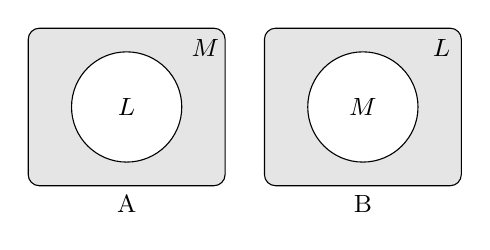
\begin{tikzpicture}[x=5mm, y=5mm,font=\small]
\definecolor{area}{gray}{0.9}
\draw [rounded corners, fill=area] (0,0) rectangle (5,4)  (4.5,3.5)node {$M$}; 
\draw[fill=white] (2.5,2) circle (1.4) node {$L$};
\node[below] at (2.5,0) {A};

\begin{scope}[xshift=30mm]
\draw [rounded corners, fill=area] (0,0) rectangle (5,4)  (4.5,3.5)node {$L$}; 
\draw[fill=white] (2.5,2) circle (1.4) node {$M$};
\node[below] at (2.5,0) {B};
\end{scope}
\end{tikzpicture}
\end{center}

\begin{definizione}
Si chiama \emph{corrispondenza} $\Kor$ \emph{fra due insiemi}~$A$ e~$B$, il 
predicato binario avente come soggetto un elemento di~$A$ e come complemento un 
elemento di~$B$.
Essa definisce un sottoinsieme~$G_\Kor$ del prodotto cartesiano~$A \times B$, 
costituito dalle coppie ordinate di elementi corrispondenti:
\[ G_\Kor=\{(a,b)\in A \times B / a \Kor b \}.\]
\end{definizione}

\osservazione
Nel capitolo precedente abbiamo chiamato relazione un predicato binario che si 
riferisce a due elementi dello stesso insieme; la differenza di terminologia
sta semplicemente nella sottolineatura del fatto che si considerano appartenenti 
allo stesso insieme oppure appartenenti a due insiemi diversi il soggetto
e il complemento del predicato binario enunciato.
A seconda del contesto in cui analizziamo un predicato binario, parleremo di 
corrispondenza o di relazione. Nelle pagine che seguono tratteremo di 
corrispondenze,
mettendo in luce le loro caratteristiche.

\begin{definizione}
Si chiama \emph{dominio} $\Dom$ di una corrispondenza l'insieme~$A$ in cui si 
trova il soggetto della proposizione vera costruita con il predicato~$\Kor$ 
\emph{codominio}~$\Cod$
l'insieme degli elementi che costituiscono il complemento della stessa 
proposizione.
\end{definizione}

Per indicare in linguaggio matematico che si è stabilita una corrispondenza tra 
due insiemi~$A$ e~$B$ scriviamo:
\[\Kor:A \rightarrow B\text{ "predicato"}, \qquad \text{oppure} \qquad \Kor:A 
\xrightarrow{\Kor:\text{ predicato}} B.\]
Formalizziamo il primo esercizio di questo capitolo:
\[\Kor:A \rightarrow B \textrm{ "significare"},\qquad \text{oppure} \qquad 
\Kor:A \xrightarrow{\Kor:\text{ significare}} B,\qquad \text{dominio } A \text{; 
codominio } B. \]

\begin{definizione}
Definita una corrispondenza~$\Kor:A \rightarrow B$, nella coppia~$(a,b)$ di 
elementi corrispondenti, $b$ si chiama \emph{immagine di}~$a$ nella 
corrispondenza~$\Kor$.
L'insieme delle immagini degli elementi del dominio è un sottoinsieme del 
codominio chiamato \emph{insieme immagine}. Verrà indicato con~$\IM$ e~$\IM 
\subseteq\Cod$.
\end{definizione}

\subsection{Rappresentazione di una corrispondenza}
\label{subsec:corr_rappresentazione}

\subsubsection{Rappresentare una corrispondenza con un grafico cartesiano}
\begin{exrig}
\begin{esempio}
Consideriamo gli insiemi~$A=$ \{Parigi, Roma, Atene\} e~$B=$ \{Italia, Francia, 
Grecia\}. Il prodotto cartesiano~$A \times B$ è rappresentato col grafico 
cartesiano della
figura~\ref{fig:C.1} (i suoi elementi sono le crocette).
Esso è formato dalle~9 coppie ordinate aventi come primo elemento una città 
(elemento di~$A$) e come secondo elemento uno stato d'Europa (elemento di~$B$).

Il predicato binario~$\Kor$: "essere la capitale di", introdotto nell'insieme~$A 
\times B$, determina il sottoinsieme~$G_\Kor$ i cui elementi sono le coppie 
(Parigi, Francia);
(Roma, Italia);(Atene, Grecia). Il dominio della corrispondenza è~$\Dom=$ 
\{Parigi, Roma, Atene\} e il codominio è~$\Cod=$ \{Italia, Francia, Grecia\} 
e~$\IM=\Cod$.
\end{esempio}
\end{exrig}

\begin{inaccessibleblock}[Figura: TODO]
 \begin{figure}[b]
\begin{minipage}[t]{.3\textwidth}
 \centering
 % (c) 2012 Dimitrios Vrettos - d.vrettos@gmail.com
\begin{tikzpicture}[ x=7.5mm, y=7.5mm, font=\small]
  \begin{scope}[->]
    \draw (0,0) -- (0,3.5) node[left] {$y$};
    \draw (0,0) -- (3.5,0) node[below] {$x$};
  \end{scope}

  \begin{scope}[Maroon, dotted, step=7.5mm]
    \draw (0,0) grid (3.5,3.5);
  \end{scope}

  \foreach \y/\ytext in {1/Italia,2/Francia,3/Grecia}{
    \node[left] at (0,\y) {\ytext};
    }

  \foreach \x/\xtext in {1/Parigi,2/Roma,3/Atene}{
    \node[below left, rotate=30] at (\x,0) {\xtext};
    }
  \foreach \x in {1,2,3}{
    \draw (\x,1.5pt) -- (\x,-1.5pt);
    \draw (1.5pt,\x) -- (-1.5pt,\x);}

  \begin{scope}[very thick, decoration={crosses, shape size=1.5mm}]
    \begin{scope}[draw=CornflowerBlue]
      \draw decorate {(1,2) -- (1,2.1)};
      \draw decorate {(2,1) -- (2,1.1)};
      \draw decorate {(3,3) -- (3,3.1)};
    \end{scope}
    \draw decorate {(1,1) -- (1,1.1)};
    \draw decorate {(2,2) -- (2,2.1)};
    \draw decorate {(3,1) -- (3,1.1)};
    \draw decorate {(2,3) -- (2,3.1)};
    \draw decorate {(1,3) -- (1,3.1)};
    \draw decorate {(3,2) -- (3,2.1)};
  \end{scope}
  \node[color=CornflowerBlue] at (3.5,3.5) {$\Cod$};
\end{tikzpicture}
 \caption{Esempio C.1.}\label{fig:C.1}
\end{minipage}\hfil
\begin{minipage}[t]{.65\textwidth}
 \centering
 % (c) 2012 Dimitrios Vrettos - d.vrettos@gmail.com
\begin{tikzpicture}[x=10mm, y=10mm, scale=.7]

  \node[ellipse, minimum height=3cm,draw, minimum width=4cm] (A) at (0,0) {};
  \node[above right] () at (A.north east) {$A$};

  \begin{scope}[fill=CornflowerBlue, every node/.style={draw=black, fill}]

    \node[circle, minimum height=1cm]  (a) at (-1.5,.5) {};
    \node[circle,fill=white, minimum height=.5cm]  at (-1.5,.5) {};
    \filldraw (.5,0) ..controls +(90:.25cm) and +(90:.5cm) .. (0,0) .. controls  +(-90:.25cm) and +(90:0cm) .. (.5,-.7) .. controls +(90:0cm) and +(-90:.25cm) ..(1,0)  ..%
    controls +(90:.5cm) and  +(90:.25cm) .. (.5,0) node[draw=CornflowerBlue,below] (h) {};

    \node[regular polygon,regular polygon sides=5, inner sep=2mm] (p) at (-1,-1.2){};

    \node [cylinder, rotate=90, minimum height=1cm, minimum width=.5cm] at (1.5,.5) (c) {};

    \node [single arrow,shape border rotate=90, minimum height=1cm, minimum width=1cm] (f) at (-.4,1.2){};
  \end{scope}

  \begin{scope}[xshift=6cm]
    \node[ellipse, minimum height=3cm,draw, minimum width=4cm] (B) at (0,0) {};

    \node[above right] () at (B.north east) {$B$};

    \node (a1) at (2,0) {anello};
    \node (h1) at (0,1.5) {cuore};
    \node (f1) at (-1.3,.75) {freccia};
    \node (p1) at (0,-1) {pentagono};
    \node (c1) at (0,0) {cilindro};
  \end{scope}
  
  \begin{scope}[->,smooth,thick]
    \draw[Maroon] (a) .. controls +(-80:2cm) and +(-150:1cm) .. (a1);
    \draw[orange] (f) .. controls +(30:2cm) and +(150:1cm) .. (f1);
    \draw[red] (c) .. controls +(-30:2cm) and +(-150:1cm) .. (c1);
    \draw[yellow] (p) .. controls +(-30:2cm) and +(-150:1cm) .. (p1);
    \draw[CornflowerBlue] (h.east) .. controls +(-30:2cm) and +(150:1cm) .. (h1.west);
  \end{scope}
\end{tikzpicture}
 \caption{Esempio C.2.}\label{fig:C.2}
\end{minipage}
\end{figure}
\end{inaccessibleblock}
% \ovalbox{\risolvii \ref{ese:C.1}, \ref{ese:C.2}}

\subsubsection{Rappresentare una corrispondenza con un grafico sagittale}

\begin{exrig}
 \begin{esempio}
 Nella figura~\ref{fig:C.2} sono rappresentati gli insiemi~$A$ e~$B$ con 
diagrammi Eulero-Venn.
 Collegando con una freccia, ciascun elemento di~$A$ con la sua forma, possiamo 
rappresentare
 con un grafico sagittale la corrispondenza~$\Kor$: ``essere di forma'', tra gli 
insiemi
 assegnati.~$A$ risulta essere il dominio e~$B$ il codominio della 
corrispondenza;~$\IM=\Cod$.
 La freccia che collega ogni elemento del dominio con la sua immagine 
rappresenta il predicato~$\Kor$.
\end{esempio}
\end{exrig}

% \ovalbox{\risolvi \ref{ese:C.3}}

\begin{exrig}
\begin{esempio}
Consideriamo gli insiemi~$R=$ \{regioni d\'Italia\} e~$M=$ \{Ligure, Ionio, 
Tirreno, Adriatico\} e la corrispondenza~$\Kor:R \rightarrow M$ "essere 
bagnata/o da"; $R$ è il dominio e~$M$
il codominio di questa corrispondenza.

L'insieme~$G_\Kor$ delle coppie ordinate aventi come primo elemento una regione 
e come secondo elemento un mare
è:~$G_\Kor=$ \{(Liguria, Ligure); (Toscana, Tirreno); (Lazio, Tirreno); 
(Campania, Tirreno); (Basilicata, Tirreno); (Calabria, Tirreno); (Calabria, 
Ionio); (Puglia, Ionio);
(Puglia, Adriatico); (Molise, Adriatico); (Abruzzo, Adriatico); (Emilia-Romagna, 
Adriatico); (Marche, Adriatico); (Veneto, Adriatico); (Friuli Venezia Giulia, 
Adriatico)\}.
Se rappresentiamo questa corrispondenza con un grafico sagittale notiamo che non 
tutti gli elementi del dominio hanno l'immagine in~$\Kor$. La corrispondenza 
definita
si può generare solo in un sottoinsieme del dominio.
\end{esempio}
\end{exrig}

\begin{definizione}
Chiamiamo \emph{insieme di definizione} della corrispondenza, indicato 
con~$\ID$, il sottoinsieme del dominio i cui elementi hanno effettivamente un 
corrispondente nel codominio.
\end{definizione}

Nel grafico (figura~\ref{fig:C.3}) è rappresentata una generica situazione 
formatasi dall'aver definito una corrispondenza tra due insiemi; sono in grigio 
l'insieme di definizione, sottoinsieme del dominio,
e l'insieme immagine, sottoinsieme del codominio.
\begin{inaccessibleblock}[Figura: TODO]
 \begin{figure}[b]
 \centering% (c) 2012 Dimitrios Vrettos - d.vrettos@gmail.com
\begin{tikzpicture}[x=10mm, y=10mm]

  \node[ellipse, minimum height=3.5cm,draw, minimum width=5cm] (D) at (0,0) {};

  \node[above] (D1) at (D.north) {$\Dom$};

  \begin{scope}[decoration={random steps,segment length=1mm}]
    \draw [decorate,fill=lightgray] (1,0)  arc (00:360:1 and 1.5) -- cycle; 
    \node [above right] at(.8,1) {$\ID$};
  \end{scope}

  \begin{scope}[fill=CornflowerBlue]
    \filldraw (0,1) circle (2pt) node (a) {};
    \filldraw (-.2,.2) circle (2pt) node (b) {};
    \filldraw (.2,-.4) circle (2pt) node (c) {};
    \filldraw (0,-1) circle (2pt) node (d) {};
    \filldraw (-1,-1) circle (2pt) ;
    \filldraw (-1.5,-.5) circle (2pt) ;
    \filldraw (-1,-1) circle (2pt) ;
    \filldraw (-2,0) circle (2pt) ;
    \filldraw (-2.2,.5) circle (2pt) ;
    \filldraw (-1,1) circle (2pt) ;
    \filldraw (-1.3,.5) circle (2pt) ;
    \filldraw (1,-1) circle (2pt) ;
    \filldraw (1.5,-.5) circle (2pt) ;
    \filldraw (1,-1) circle (2pt) ;
    \filldraw (2,0) circle (2pt) ;
    \filldraw (2.2,.5) circle (2pt) ;
    \filldraw (1.3,.5) circle (2pt) ;
  \end{scope}

  \begin{scope}[xshift=6cm]
    \node[ellipse, minimum height=3.5cm,draw, minimum width=5cm] (C) at (0,0) {};
    \node[above] (C1) at (C.north) {$\Cod$};

    \begin{scope}[decoration={random steps,segment length=1mm}]
      \draw [decorate,fill=lightgray] (1,0)  arc (00:360:1 and 1.5) -- cycle; 
      \node [above right] at(.8,1) {$\IM$};
    \end{scope}
    
    \begin{scope}[fill=LimeGreen]
      \filldraw (0,1) circle (2pt) node (a1) {};
      \filldraw (-.2,.2) circle (2pt) node (b1) {};
      \filldraw (.2,-.4) circle (2pt) node (c1) {};
      \filldraw (0,-1) circle (2pt) node (d1) {};

      \filldraw (-1,-1) circle (2pt) ;
      \filldraw (-1.5,-.5) circle (2pt) ;
      \filldraw (-1,-1) circle (2pt) ;
      \filldraw (-2,0) circle (2pt) ;
      \filldraw (-2.2,.5) circle (2pt) ;

      \filldraw (-1.3,.5) circle (2pt) ;
      \filldraw (1.5,-.5) circle (2pt) ;
      \filldraw (1,-1) circle (2pt) ;
      \filldraw (2,0) circle (2pt) ;
      \filldraw (2.2,.5) circle (2pt) ;
    \filldraw (1.3,.5) circle (2pt) ;
    \end{scope}
  \end{scope}
  
  \begin{scope}[->,smooth,thick]
    \draw[blue] (D1.north) .. controls +(80:1cm) and +(80:1cm) .. (C1.north) node [midway, above, black] () {$\Kor$};
    \draw[Maroon] (a) .. controls +(80:1cm) and +(150:1cm) .. (a1);
    \draw[orange] (b) .. controls +(30:2cm) and +(150:1cm) .. (b1);
    \draw[red] (c) .. controls +(-30:2cm) and +(-150:1cm) .. (c1);
    \draw[yellow] (d) .. controls +(-30:2cm) and +(-150:1cm) .. (d1);
  \end{scope}
\end{tikzpicture}
 \caption{Corrispondenza tra due insiemi.}\label{fig:C.3}
\end{figure}
\end{inaccessibleblock}

Osserviamo che in alcuni casi si ha la coincidenza del dominio con l'insieme di 
definizione e la coincidenza del dominio con l'insieme immagine:~$\Dom=\ID$ 
e~$\Cod=\IM$.

% \newpage
% 
% \subsection{Caratteristiche di una corrispondenza}
% \label{subsec:corr_caratteristiche}
% 
% \begin{exrig}
% \begin{esempio}
% Generalizziamo uno degli esercizi precedenti sulle date di nascita. Prendiamo 
% come dominio~$\Dom=$ \{persone italiane viventi\} e come codominio~$\Cod=$ \{gli 
% anni dal~1900 al~2012\}.
% Evidentemente~$\ID=\Dom$: ogni persona ha un determinato anno di nascita, ma più 
% persone sono nate nello stesso anno. Inoltre~$\IM$ potrebbe coincidere 
% con~$\Cod$,
% vista la presenza sul territorio nazionale di ultracentenari. Comunque 
% scriveremo~$\IM \subseteq \Cod$. Il grafico sagittale di questa corrispondenza è 
% del tipo rappresentato nella
% figura~\ref{fig:C.4}.
% \end{esempio}
% \begin{inaccessibleblock}[Figura: TODO]
%  \begin{figure}[t]
%  \centering% (c) 2012 Dimitrios Vrettos - d.vrettos@gmail.com
\begin{tikzpicture}[x=10mm, y=10mm]

  \node[ellipse, minimum height=3cm,draw, minimum width=4cm] (D) at (0,0) {};

  \node[above] (D1) at (D.north) {$\Dom$};

  \begin{scope}[fill=CornflowerBlue]
    \filldraw (0,1) circle (2pt) node (a) {};
    \node[above left] at (0,1) {$p_1$};
    \filldraw (-.2,.2) circle (2pt) node (b) {};
    \node[above left] at (-.2,.2) {$p_2$};
    \filldraw (.2,-.4) circle (2pt) node (c) {};
    \node[above left] at (.2,-.4) {$p_3$};
    \filldraw (0,-1) circle (2pt) node (d) {};
    \node[above left] at (0,-1) {$p_4$};
    \filldraw (-1,-1) circle (2pt) node (e) {};
    \node[above left] at (-1,-1) {$p_5$};
    \filldraw (-1.5,-.5) circle (2pt) ;
    \filldraw (-1,-1) circle (2pt) ;
    \filldraw (-1,1) circle (2pt) ;
    \filldraw (-1.3,.5) circle (2pt) ;
    \filldraw (1,-1) circle (2pt) ;
    \filldraw (1.5,-.5) circle (2pt) ;
    \filldraw (1,-1) circle (2pt) ;
    \filldraw (1.3,.5) circle (2pt) ;
  \end{scope}

  \begin{scope}[xshift=5cm]
    \node[ellipse, minimum height=3.cm,draw, minimum width=4cm] (C) at (0,0) {};

    \node[above] (C1) at (C.north) {$\Cod$};

    \begin{scope}[fill=LimeGreen]
    \filldraw (0,1) circle (2pt) node (a1) {};
    \filldraw (-.2,.2) circle (2pt);
    \filldraw (.2,-.4) circle (2pt) node (c1) {};
    \filldraw (0,-1) circle (2pt);

    \node[above right]  at (0,1) {1910};
    \node[above right]  at (.2,-.4) {1997};
    \filldraw (-1,-1) circle (2pt) ;
    \filldraw (-1.5,-.5) circle (2pt) ;
    \filldraw (-1,-1) circle (2pt) ;
    \filldraw (-1.3,.5) circle (2pt) ;
    \filldraw (1.5,-.5) circle (2pt) ;
    \filldraw (1,-1) circle (2pt) ;
    \filldraw (1.3,.5) circle (2pt) ;
    \end{scope}
  \end{scope}

  \begin{scope}[->,smooth,thick]
    \draw[blue] (D1.north) .. controls +(80:1cm) and +(80:1cm) .. (C1.north) node [midway, above, black] () {$\Kor$};
    \draw[Maroon] (a) .. controls +(80:1cm) and +(150:1cm) .. (a1);
    \draw[orange] (b) .. controls +(30:2cm) and +(150:1cm) .. (c1);
    \draw[red] (c) .. controls +(-30:2cm) and +(-150:1cm) .. (c1);
    \draw[yellow] (d) .. controls +(-30:2cm) and +(-180:2cm) .. (c1);
    \draw[purple] (e) .. controls +(-30:2cm) and +(-150:1cm) .. (a1);
  \end{scope}
\end{tikzpicture}
%  \caption{Corrispondenza \emph{molti a uno}: più persone sono nate nello stesso 
% anno.}\label{fig:C.4}
% \end{figure}
% \end{inaccessibleblock}
% 
% \begin{esempio}
% Analizziamo la corrispondenza dell'esempio precedente~$\Kor:R \rightarrow M$ 
% ``essere bagnata/o da'' tra l'insieme delle regioni d'Italia e l'insieme dei 
% mari. 
% 
% $\ID\subset\Dom$ poiché alcune regioni non sono bagnate da alcun mare. Moltre 
% regioni sono bagnate dallo stesso mare, ma succede che alcune regioni siano 
% bagnate da
% due mari. 
% 
% $IM=C$: un mare bagna almeno una regione. Il grafico sagittale di questa 
% corrispondenza è del tipo rappresentato nella
% figura~\ref{fig:C.5}.
% \end{esempio}
% 
% \begin{inaccessibleblock}[Figura: TODO]
%  \begin{figure}[t]
%  \centering% (c) 2012 Dimitrios Vrettos - d.vrettos@gmail.com
\begin{tikzpicture}[x=10mm, y=10mm]

\node[ellipse, minimum height=3cm,draw, minimum width=4cm] (D) at (0,0) {};

\node[above] (D1) at (D.north) {Regioni};

\draw[dotted] (-.6,1.4) -- (-.6,-1.4);
\begin{scope}[fill=CornflowerBlue]

\filldraw (.7,1) circle (2pt) node (a) {};
\node[left] at (.7,1) {Liguria};
\filldraw (1,.2) circle (2pt) node (b) {};
\node[left] at (1,.2) {Calabria};
\filldraw (.8,-.5) circle (2pt) node (c) {};
\node[left] at (.8,-.5) {Puglia};
\filldraw (-1.3,0) circle (2pt) node (d) {};
\node[above] at (-1.3,0) {Umbria};

\node at (.4,-1) {$\ID$};
\end{scope}

\begin{scope}[xshift=5cm]
\node[ellipse, minimum height=3cm,draw, minimum width=4cm] (C) at (0,0) {};

\node[above] (C1) at (C.north) {Mari};

\begin{scope}[fill=LimeGreen]
\filldraw (-.2,1) circle (2pt) node (a1) {};
\filldraw (-.2,.2) circle (2pt)node (b1) {};
\filldraw (.2,-.4) circle (2pt) node (c1) {};
\filldraw (0,-1) circle (2pt) node (d1){};

\node[right]  at (-.2,1) {Adriatico};
\node[right]  at (.2,-.4) {Ionio};
\node[right] at (-.2,.2) {Tirreno};
\node[right] at (0,-1) {Ligure};

\end{scope}
\end{scope}
\begin{scope}[->,smooth,thick]
\draw[blue] (D1.north) .. controls +(80:1cm) and +(80:1cm) .. (C1.north) node [midway, above, black] () {$\Kor$};
\draw[Maroon] (a) .. controls +(80:1cm) and +(150:1cm) .. (d1);
 \draw[orange] (b) .. controls +(30:2cm) and +(150:1cm) .. (c1);
\draw[orange] (b) .. controls +(-30:2cm) and +(-150:1cm) .. (b1);
\draw[red] (c) .. controls +(-30:2cm) and +(-180:2cm) .. (c1);
\draw[red] (c) .. controls +(-30:2cm) and +(-180:2cm) .. (a1);
\end{scope}
\end{tikzpicture}
%  \caption{Esempio di corrispondenza di tipo \emph{molti a 
% molti}.}\label{fig:C.5}
% \end{figure}
% \end{inaccessibleblock}
% 
% \begin{esempio}
% Generalizziamo la corrispondenza~$\Kor$: ``essere la capitale di'' tra il 
% dominio~$\Cod=$ \{città d'Europa\} e il codominio~$S=$ \{stati d'Europa\}. È 
% evidente che~$\ID\subset\Cod$:
% non tutte le città sono capitali, mentre~$\IM=\Cod$ in quanto ogni stato ha la 
% sua capitale; inoltre due città diverse non possono essere capitali dello stesso 
% stato.
% Il grafico sagittale di questa corrispondenza è del tipo rappresentato nella
% figura~\ref{fig:C.6}.
% \end{esempio}
% 
% \begin{inaccessibleblock}[Figura: TODO]
%  \begin{figure}[t]
%  \centering% (c) 2012 Dimitrios Vrettos - d.vrettos@gmail.com
\begin{tikzpicture}[x=10mm, y=10mm]

\node[ellipse, minimum height=3cm,draw, minimum width=4cm] (D) at (0,0) {};

\node[above] (D1) at (D.north) {Città};

\draw[dotted] (-.6,1.4) -- (-.6,-1.4);
\begin{scope}[fill=CornflowerBlue]

\filldraw (.7,1) circle (2pt) node (a) {};
\node[left] at (.7,1) {Roma};
\filldraw (1,.2) circle (2pt) node (b) {};
\node[left] at (1,.2) {Parigi};
\filldraw (.8,-.5) circle (2pt) node (c) {};
\node[left] at (.8,-.5) {Londra};
\filldraw (-1.3,0) circle (2pt) node (d) {};
\node[above] at (-1.3,0) {Genova};

\node at (.4,-1) {$\ID$};
\end{scope}

\begin{scope}[xshift=5cm]
\node[ellipse, minimum height=3cm,draw, minimum width=4cm] (C) at (0,0) {};

\node[above] (C1) at (C.north) {Stati};

\begin{scope}[fill=LimeGreen]
\filldraw (-.1,1) circle (2pt) node (a1) {};
\filldraw (-.2,.2) circle (2pt)node (b1) {};
\filldraw (.2,-.8) circle (2pt) node (c1) {};

\node[right]  at (-.1,1) {Francia};
\node[right]  at (.2,-.8) {Italia};
\node[right] at (-.2,.2) {Inghilterra};

\end{scope}
\end{scope}
\begin{scope}[->,smooth,thick]
\draw[blue] (D1.north) .. controls +(80:1cm) and +(80:1cm) .. (C1.north) node [midway, above, black] () {$\Kor$};
\draw[Maroon] (a) .. controls +(30:1cm) and +(150:1cm) .. (c1);
 \draw[orange] (b) .. controls +(30:2cm) and +(150:1cm) .. (a1);
\draw[red] (c) .. controls +(-30:2cm) and +(-180:2cm) .. (b1);
\end{scope}
\end{tikzpicture}
%  \caption{Esempio di corrispondenza di tipo \emph{uno a uno}.}\label{fig:C.6}
% \end{figure}
% \end{inaccessibleblock}
% \begin{esempio}
% Consideriamo, tra l'insieme~$\insN_0$ dei numeri naturali diversi da zero e 
% l'insieme~$\insZ_0$ degli interi relativi diversi da zero, la 
% corrispondenza~$\Kor$: ``essere il valore assoluto di''.
% Per la definizione di valore assoluto di un intero, possiamo senz'altro 
% dire:~$\insN_0=\Dom=\ID$ $\insZ_0=\Cod=\IM$. Ma succede che due numeri opposti 
% hanno lo stesso valore assoluto,
% quindi ogni elemento di~$\mathbb{N}_0$ ha due immagini, per cui il grafico 
% sagittale di questa corrispondenza è come nella figura~\ref{fig:C.7}.
% \end{esempio}
% \begin{inaccessibleblock}[Figura: TODO]
%  \begin{figure}[t]
%  \centering% (c) 2012 Dimitrios Vrettos - d.vrettos@gmail.com
\begin{tikzpicture}[x=10mm, y=10mm]

\node[ellipse, minimum height=3cm,draw, minimum width=4cm] (D) at (0,0) {};

\node[above] (D1) at (D.north) {$\Dom=\insN_0$};

\begin{scope}[fill=CornflowerBlue]

\filldraw (0,1) circle (2pt) node (a) {};
\node[left] at (0,1) {1};
\filldraw (1,.2) circle (2pt) node (b) {};
\filldraw (0,-.5) circle (2pt) node (c) {};
\node[left] at (0,-.5) {5};
\filldraw (-1.3,0) circle (2pt) node (d) {};


\end{scope}

\begin{scope}[xshift=5cm]
\node[ellipse, minimum height=3cm,draw, minimum width=4cm] (C) at (0,0) {};

\node[above] (C1) at (C.north) {$\Cod=\insZ_0$};

\begin{scope}[fill=LimeGreen]
\filldraw (-.1,1) circle (2pt) node (a1) {};
\filldraw (-.5,.5) circle (2pt)node (b1) {};
\filldraw (.2,-.8) circle (2pt) node (c1) {};
\filldraw  (-.2,0) circle (2pt) node (d1){};
\filldraw  (.8,1) circle (2pt);
\filldraw  (1.5,0) circle (2pt);
\node[right]  at (-.1,1) {$+1$};
\node[right]  at (-.5,.5) {$-1$};
\node[right]  at (.2,-.8) {$-5$};
\node[right] at (-.2,0) {$+5$};

\end{scope}
\end{scope}
\begin{scope}[->,smooth,thick]
\draw[blue] (D1.north) .. controls +(80:1cm) and +(80:1cm) .. (C1.north) node [midway, above, black] () {$\Kor$};
\draw[Maroon] (a) .. controls +(30:1cm) and +(150:1cm) .. (a1);
 \draw[Maroon] (a) .. controls +(30:1cm) and +(150:1cm) .. (b1);
\draw[red] (c) .. controls +(-30:2cm) and +(-180:2cm) .. (c1);
\draw[red] (c) .. controls +(-30:2cm) and +(-180:2cm) .. (d1);
\end{scope}
\end{tikzpicture}

%  \caption{Esempio di corrispondenza di tipo \emph{uno a molti}.}\label{fig:C.7}
% \end{figure}
% \end{inaccessibleblock}
% \end{exrig}
% 
% \begin{definizione}
% Le corrispondenze di tipo \emph{molti a uno} e \emph{uno a uno} sono dette 
% \emph{univoche}; in esse ogni elemento dell'insieme di definizione ha una sola 
% immagine nel codominio.
% \end{definizione}
% %\newpage
% \begin{exrig}
% \begin{esempio}
% Consideriamo la corrispondenza~$\Kor$ che associa ad ogni persona il suo codice 
% fiscale: ogni persona ha il proprio codice fiscale, persone diverse hanno codice 
% fiscale diverso.
% Dominio e~$\ID$ coincidono e sono l'insieme~$P=$ \{persone\}. Codominio e~$\IM$ 
% coincidono e sono l'insieme~$F=$ \{codici fiscali\}. Il grafico sagittale di 
% questa corrispondenza
% è del tipo \emph{uno a uno}. È di questo tipo il grafico sagittale della 
% corrispondenza che associa ad ogni automobile la sua targa, ad ogni moto il suo 
% numero di telaio,
% ad ogni maggiorenne, cittadino italiano, il suo certificato elettorale \ldots
% 
% \end{esempio}
% \end{exrig}
% 
% \osservazione In tutti questi casi la corrispondenza è di tipo \emph{uno a uno}, 
% il dominio coincide con l'insieme di definizione e l'insieme immagine coincide 
% con il codominio.
% 
% \begin{definizione}
% Una corrispondenza di tipo \emph{uno a uno} in cui~$\Dom=\ID$ e~$\Cod=\IM$ è 
% detta \emph{corrispondenza biunivoca}.
% \end{definizione}
% 
% %\ovalbox{\risolvii \ref{ese:C.4}, \ref{ese:C.5}, \ref{ese:C.6}, \ref{ese:C.7}, 
% % \ref{ese:C.8}, \ref{ese:C.9}, \ref{ese:C.10}}

\end{comment}

\section{Relazioni in un insieme}
\label{sec:relazioni}

Il termine \emph{relazione} entra molto spesso in frasi del linguaggio naturale, 
lo usiamo per esprimere un generico legame tra due persone o tra due oggetti,
anche senza specificarne la natura: ``si è conclusa la relazione tra Anna e 
Paolo'', ``l'allungamento di una sbarretta di ferro è in relazione con il calore 
fornito'',
``la frana del terreno è in relazione con il disboscamento della zona e 
l'abusivismo edilizio'', ``domani consegnerò la relazione di fisica''.
Sono tutte espressioni che ci danno informazioni di un qualche collegamento tra 
gli
argomenti (persone, cose) ai quali il termine relazione si riferisce.

Dal punto di vista matematico diamo la seguente definizione.
\begin{definizione}
Si dice \emph{relazione} in un insieme~$A$ un predicato binario che lega due 
elementi dell'insieme.
\end{definizione}

\begin{exrig}
 \begin{esempio}
 Nell'insieme~$A = \lbrace~3, 5, 6, 9, 30 \rbrace$ è introdotto il predicato 
binario ``essere multiplo di''; con esso formiamo le proposizioni vere 
scegliendo soggetto e
 complemento nell'insieme~$A$:

\begin{multicols}{3}
30 è multiplo di~6;

9 è multiplo di~3;

30 è multiplo di~3;

6 è multiplo di~3;

30 è multiplo di~5;

3 è multiplo di~3;

5 è multiplo di~5;

6 è multiplo di~6;

9 è multiplo di~9;

30 è multiplo di~30.
\end{multicols}
Il predicato ``essere multiplo'' genera nell'insieme~$A$ una relazione 
matematica. Esso tuttavia non è il
solo che permette di collegare tra loro due elementi di quell'insieme.
\end{esempio}
\end{exrig}

% \ovalbox{\risolvi \ref{ese:B.2}}

Se chiamiamo con~$\Rel$ il predicato binario che definisce la relazione 
introdotta nell'insieme, per indicare sinteticamente
che la proposizione avente come soggetto~$a$, come complemento~$b$ e come 
predicato~$\Rel$, scriviamo~$a \Rel b$ e
diremo sinteticamente che~\emph{$a$ è in relazione con~$b$}.

\begin{exrig}
 \begin{esempio}

Con riferimento all'esempio precedente si ha:~$A = \lbrace~3,5,6,9,30 \rbrace$, 
$\Rel$:
``essere multiplo di''. Allora scriviamo: per qualunque~$a$ e~$b$ appartenenti 
ad~$A$,
$a \Rel b$ se e solo se~$a$ è multiplo di~$b$, in particolare:
\[30 \Rel~6;\quad~9 \Rel~3;\quad~30 \Rel~3;\quad~6 \Rel~3;\quad~30 
\Rel~5;\quad~3 \Rel~3;\quad~5 \Rel~5;\quad~6 \Rel~6;\quad~9 \Rel~9;\quad~30 
\Rel~30.\]
\end{esempio}
\end{exrig}

Abbiamo così formato un insieme di \emph{coppie ordinate} di elementi tra loro 
in relazione:~$30 \Rel~5$ può anche essere indicata con~$(30,5)$.

\begin{definizione}
Chiamiamo \emph{insieme della relazione} (in simboli~$G_\Rel$) l'insieme delle 
coppie ordinate i cui
elementi sono gli argomenti del predicato binario, ossia sono in relazione tra 
di loro. Esso risulta essere un
sottoinsieme del prodotto cartesiano dell'insieme~$A$ con se stesso. Si 
rappresenta per proprietà caratteristica nel
seguente modo~$G_\Rel = \lbrace (a,b) \in A \times A / a \Rel b \rbrace$.
\end{definizione}

% \ovalbox{\risolvii \ref{ese:B.3}, \ref{ese:B.4}, \ref{ese:B.5}, \ref{ese:B.6}}

\begin{comment}
 
%===================================
\subsection{Rappresentazioni di una relazione}
\label{subsec:rel_rappresentazione}

\subsubsection{Grafico di una relazione}

Dal momento che una relazione in un insieme~$Y$ determina un sottoinsieme del 
prodotto cartesiano~$Y \times Y$ è
comodo rappresentare una relazione nello stesso diagramma usato per 
rappresentare il prodotto cartesiano.
Una relazione può quindi essere rappresentata attraverso un \emph{grafico 
cartesiano}.

% \ovalbox{\risolvii \ref{ese:B.7}, \ref{ese:B.8}}

%===================================
\subsubsection{Matrice o tabella di una relazione}

Nella figura~\ref{fig:B.1} è rappresentata la classica griglia per il gioco 
della battaglia navale.
Ogni cella è individuata da una coppia ordinata il cui primo elemento (una 
lettera dell'alfabeto) indica la riga,
il secondo (un numero) indica la colonna; così la coppia~$(D,5)$ indica la cella 
annerita.


% \ovalbox{\risolvii \ref{ese:B.9}, \ref{ese:B.10}, \ref{ese:B.11}}

%===================================
\subsubsection{Grafo di una relazione}

\begin{definizione}
Un \emph{grafo} è un insieme di punti detti nodi e di archi che uniscono coppie 
di punti.
\end{definizione}

Abbiamo visto che con un predicato si possono formare alcune proposizioni aventi 
rispettivamente come soggetto e
come complemento elementi di un insieme: solo le proposizioni vere determinano 
la relazione tra gli elementi di
quell'insieme e generano coppie di elementi in relazione.

\begin{exrig}
 \begin{esempio}

Nel diagramma di Eulero-Venn (figura~\ref{fig:B.2}) dell'insieme~$A = \lbrace~3, 
5, 6, 9, 30 \rbrace$
rappresentiamo la relazione~$\Rel$ = ``essere multiplo di'' collegando mediante 
una freccia gli argomenti delle proposizione vere.


Come puoi osservare l'elemento~30 è collegato con una freccia all'elemento~6 in 
quanto la proposizione: ``30 è multiplo di~6'' è vera, ma non all'elemento~9
poiché la proposizione: ``30 è multiplo di~9'' è falsa; inoltre la punta della 
freccia è sul numero~6 in quanto complemento del predicato ``essere multiplo'';
infine su ciascun elemento abbiamo messo un \emph{anello} o \emph{cappio} per 
indicare che ogni elemento è in relazione con se stesso essendo vera per ogni
elemento~$a$ dell'insieme~$A$ la proposizione: ``$a$ è multiplo di~$a$''.

 \end{esempio}
\end{exrig}

% \ovalbox{\risolvii \ref{ese:B.12}, \ref{ese:B.13}, \ref{ese:B.14}, 
% \ref{ese:B.15}, \ref{ese:B.16}, \ref{ese:B.17}, \ref{ese:B.18}}

\begin{inaccessibleblock}[Figura: TODO]
 \begin{figure}[b]
\begin{minipage}[t]{.45\textwidth}
 \centering
 % (c) 2012 Dimitrios Vrettos - d.vrettos@gmail.com

\begin{tikzpicture}[x=10mm,y=10mm, font=\small,table nodes/.style={%
		rectangle,
		draw=black,
 		align=center,
   		minimum height=5mm,
     	text depth=0.5ex,
     	text height=1.5ex,
     	inner xsep=-1pt,
     	outer sep=0pt
	},
	table/.style={%
        matrix of nodes,
        row sep=-\pgflinewidth,
        column sep=-\pgflinewidth,
        nodes={%
            table nodes
        },
        execute at empty cell={\node[fill=black]{};}
    }]

\matrix (first) [table,text width=7mm,name=table]
{
{}  & 1 & 2 & 3 &4 & 5 & 6 & 7\\
$A$ &{} &{} &{} &{} &{} &{} &{} \\
$B$ &{} &{} &{} &{} &{} &{} &{} \\
$C$ &{} &{} &{} &{} &{} &{} &{} \\
$D$ &{} &{} &{} &{} & &{} &{}  \\
$E$ &{} &{} &{} &{} &{} &{} &{} \\
$F$ &{} &{} &{} &{} &{} &{} &{} \\
};

\end{tikzpicture}

 \caption{Griglia della battaglia navale.}\label{fig:B.1}
\end{minipage}\hfil
\begin{minipage}[t]{.45\textwidth}
 \centering
 % (c) 2012 Dimitrios Vrettos - d.vrettos@gmail.com

\begin{tikzpicture}[x=10mm,y=10mm, font=\small, every state/.style={draw=CornflowerBlue}, every loop/.style={draw=Maroon}]
\draw (0,0) circle (2);

\node[state] (5) at (-1.5,0) {5};
\node[state] (30) at (-.4,.8) {30};
\node[state] (6) at (1.1,.5) {6};
\node[state] (9) at (1,-1) {9};
\node[state] (3) at (-.5,-1.2) {3};

\begin{scope}[->]
\path(5) edge[loop below] node{} ()
	(30) edge[loop above] node{} ()
	(6) edge[loop above] node{} ()
	(9) edge[loop above] node{} ()
	(3) edge[loop left] node{} ();

\end{scope}
\begin{scope}[->, Maroon]
\draw (30)--(5);
\draw (30)--(6);
\draw (30)--(3);
\draw (6)--(3);
\draw (9)--(3);
\end{scope}
\end{tikzpicture}

 \caption{L'insieme~$A$.}\label{fig:B.2}
\end{minipage}
\end{figure}
\end{inaccessibleblock}

\end{comment}

\subsection{Proprietà delle relazioni}
\label{subsec:rel_proprieta}

%===================================
\subsubsection{Proprietà riflessiva}

\begin{exrig}
 \begin{esempio}

Nell'insieme~$T = \lbrace~7, 8, 12, 34, 100 \rbrace$ è introdotta la 
relazione~$\Rel$: ``essere divisore di''.
Puoi osservare che ogni numero è divisore di se stesso, cioè ogni elemento 
dell'insieme è in relazione
con se stesso. Una relazione di questo tipo si dice che gode della 
\emph{proprietà riflessiva}.
Osserva, però, che nell'insieme ~$\insN$ dei numeri naturali la relazione 
``essere divisibile per'' non è riflessiva poiché zero non è divisibile per se 
stesso.
 \end{esempio}
\end{exrig}

\begin{definizione}
Una relazione~$\Rel$ in un insieme~$A$ gode della \emph{proprietà riflessiva} 
quando ogni elemento è in relazione con se stesso, ossia per qualunque~$x$
dell'insieme~$A$ si ha~$x \Rel x$.
\end{definizione}

% \ovalbox{\risolvi \ref{ese:B.19}}

%===================================
\subsubsection{Proprietà antiriflessiva}

\begin{exrig}
 \begin{esempio}
Nell'insieme delle persone~$P = \lbrace\text{Marco, Antonio, Carlo}\rbrace$ è 
data la relazione~$\Rel$: ``essere più alto''
rappresentata con la figura~\ref{fig:B.3}.
Puoi notare che nessun elemento è in relazione con se stesso. In effetti nessuno 
può ``essere più alto'' di se stesso.

 \end{esempio}
\end{exrig}

\begin{definizione}
Una relazione~$\Rel$ in un insieme~$A$ gode della \emph{proprietà 
antiriflessiva} quando nessun elemento è in relazione con se stesso,
ossia per nessun elemento~$x$ di~$A$ si ha~$x \Rel x$.
\end{definizione}

% \ovalbox{\risolvi \ref{ese:B.20}}
\subsubsection{Proprietà simmetrica}

\begin{exrig}
 \begin{esempio}
Nella figura~\ref{fig:B.4} è rappresentata la relazione~$\Rel$: ``essere 
concorde con'' nell'insieme dei 
numeri~$A = \lbrace -1,~+3,~-7,~+5,~-2,~+4,~+10 \rbrace$.
Per collegare elementi in relazione abbiamo usato archi poiché, ad esempio, le 
proposizioni ``$+3$ è concorde con~$+10$'' e ``$+10$ è concorde con~$+3$''
sono entrambe vere. Per questa relazione si può osservare che se un elemento 
dell'insieme è in relazione con un altro allora anche quest'ultimo
è in relazione con il primo:
$-1~\Rel~-7$, ma anche~$-7~\Rel~-1$ $+3~\Rel~+5$, ma anche~$+5~\Rel~+3$ e così 
via.
 \end{esempio}
\end{exrig}

\begin{inaccessibleblock}[Figura: TODO]
 \begin{figure}[t]
\begin{minipage}[t]{.45\textwidth}
 \centering
 % (c) 2012 Dimitrios Vrettos - d.vrettos@gmail.com

\begin{tikzpicture}[x=10mm,y=10mm, font=\small, every state/.style={draw=CornflowerBlue}, every loop/.style={draw=Maroon}]
\draw (0,0) circle (1.8);

\node at (1.8,1.5) {$P$};

\node[state] (M) at (-1,.3) {$M$};
\node[state] (C) at (.8,.8) {$C$};
\node[state] (A) at (.2,-1) {$A$};

 \begin{scope}[->, Maroon]
 \draw (M)--(C);
 \draw (M)--(A);
 \draw (C)--(A);
 \end{scope}
\end{tikzpicture}
 \caption{Proprietà antiriflessiva.}\label{fig:B.3}
\end{minipage}\hfil
\begin{minipage}[t]{.45\textwidth}
 \centering
 % (c) 2012 Dimitrios Vrettos - d.vrettos@gmail.com

\begin{tikzpicture}[x=10mm,y=10mm, font=\small, every state/.style={draw=CornflowerBlue}, every loop/.style={draw=Maroon}]
\draw (0,0) circle [x radius=3, y radius=2];

\node[state] (A) at (-2.3,.3) {$-1$};
\node[state] (B) at (-.8,1.2) {$-2$};
\node[state] (C) at (-1.5,-1) {$-7$};
\node[state] (D) at (-.5,-.9) {$+10$};
\node[state] (E) at (.6,.9) {$+3$};
\node[state] (F) at (1.8,.5) {$+4$};
\node[state] (G) at (1.5,-1) {$+5$};

\begin{scope}[->]
\path(A) edge[loop below] node{} ()
	(B) edge[loop right] node{} ()
	(C) edge[loop left] node{} ()	
(D) edge[loop below] node{} ()
	(E) edge[loop above] node{} ()
	(F) edge[loop right] node{} ()
	(G) edge[loop right] node{} ();

\end{scope}
% \begin{scope}[<->, Maroon]
 \begin{scope}[-, Maroon]
 \draw (A)--(C);
 \draw (B)--(A);
 \draw (C)--(B);
\draw (D)--(E);
\draw (D)--(F);
\draw (E)--(F);
\draw (G)--(F);
\draw (E)--(G);
\draw (D)--(G);
 \end{scope}
\end{tikzpicture}

 \caption{Proprietà simmetrica.}\label{fig:B.4}
\end{minipage}
\end{figure}
\end{inaccessibleblock}

\begin{definizione}
Una relazione~$\Rel$ introdotta in un insieme~$A$ gode della \emph{proprietà 
simmetrica} quando risultano vere le due proposizioni
che si ottengono scambiando soggetto e complemento; ossia per qualunque~$x$ 
e~$y$ appartenenti all'insieme~$A$ se vale~$x \Rel y$
allora vale anche~$y \Rel x$.
\end{definizione}

% \ovalbox{\risolvi \ref{ese:B.21}}

%===================================
\subsubsection{Proprietà antisimmetrica}

\begin{exrig}
 \begin{esempio}

Il diagramma di Venn, nella figura~\ref{fig:B.5}, rappresenta un insieme~$U$ e 
alcuni suoi sottoinsiemi.

Consideriamo ora l'insieme di insiemi~$S = \lbrace U, A, B, C, D, E, F \rbrace$ 
e la relazione~$\Rel$: ``essere sottoinsieme proprio di'':
completa il grafo della relazione.

Certamente nel completare il grafo (figura~\ref{fig:B.6}) non avrai usato archi: 
è evidente che le proposizioni ``$B$ è sottoinsieme proprio di~$C$'' e ``$C$
è sottoinsieme proprio di~$B$'' non possono essere entrambe vere. Anzi, la 
verità della prima implica necessariamente la falsità della seconda.
 \end{esempio}
\end{exrig}

\begin{inaccessibleblock}[Figura: TODO]
 \begin{figure}[b]
\begin{minipage}[b]{.45\textwidth}
 \centering
 % (c) 2012 Dimitrios Vrettos - d.vrettos@gmail.com

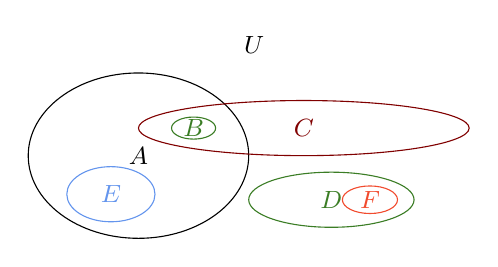
\begin{tikzpicture}[scale=.7,x=10mm,y=10mm, font=\small, every state/.style={draw=CornflowerBlue}, every loop/.style={draw=Maroon}]
\draw (0,0) circle [x radius=2, y radius=1.5] node {$A$};
\draw[CornflowerBlue] (-.5,-.7) circle [x radius=.8, y radius=.5]node {$E$};
\draw[OliveGreen] (1,.5) circle [x radius=.4, y radius=.2]node {$B$};
\draw[Maroon] (3,.5) circle [x radius=3, y radius=.5]node {$C$};
\draw[OliveGreen] (3.5,-.8) circle [x radius=1.5, y radius=.5]node {$D$};
\draw[RedOrange] (4.2,-.8) circle [x radius=.5, y radius=.25]node {$F$};

\node () at (2.1,2) {$U$};
\end{tikzpicture}
 \caption{L'insieme~$U$.}\label{fig:B.5}
\end{minipage}\hfil
\begin{minipage}[b]{.45\textwidth}
 \centering
 % (c) 2012 Dimitrios Vrettos - d.vrettos@gmail.com

\begin{tikzpicture}[scale=.7,x=10mm,y=10mm, font=\small, every state/.style={draw=CornflowerBlue}, every loop/.style={draw=Maroon}]
\draw (0,0) circle [x radius=3, y radius=2];

\node at (3,1.5) {$S$};
\node[state] (A) at (-2.3,.3) {$A$};
\node[state] (B) at (-.8,1.2) {$B$};
\node[state] (C) at (-1.5,-1) {$C$};
\node[state] (D) at (-.2,-1.1) {$D$};
\node[state] (E) at (.6,.9) {$E$};
\node[state] (F) at (1.8,.5) {$F$};
\node[state] (U) at (1.5,-1) {$U$};

  \begin{scope}[->, Maroon]
 \draw (A)--(U);
  \draw (B)--(C);
 \draw (F)--(U);
   \end{scope}
\end{tikzpicture}
 \caption{L'insieme~$S$.}\label{fig:B.6}
\end{minipage}
\end{figure}
\end{inaccessibleblock}

\begin{definizione}
Una relazione~$\Rel$ introdotta in un insieme~$A$ gode della \emph{proprietà 
antisimmetrica} quando non possono essere vere
contemporaneamente le proposizioni che si ottengono scambiando il soggetto con 
il complemento, se soggetto e complemento sono diversi
tra loro; ossia per qualunque~$x$ e~$y$ dell'insieme~$A$ se~$x \neq y$ e se~$x 
\Rel y$ non è vero che~$y \Rel x$.
\end{definizione}

% \ovalbox{\risolvi \ref{ese:B.22}}

%===================================
\subsubsection{Proprietà transitiva}

\begin{exrig}
 \begin{esempio}

Nel grafo (figura~\ref{fig:B.7}) è rappresentata una relazione~$\Rel$ introdotta 
in un insieme~$T$. Dall'analisi della situazione rappresentata possiamo
affermare che dalla verità di ($a \Rel b$ e~$b \Rel c$) segue la verità di~$a 
\Rel c$. Analizzando gli altri elementi, 
possiamo osservare che essendo vera ($e \Rel f$ e~$f \Rel g$) è vera anche~$e 
\Rel g$
inoltre si ha che essendo vera ($n \Rel m$ e~$m \Rel t$) è vera anche~$n \Rel 
t$.
 \end{esempio}
\end{exrig}

\begin{inaccessibleblock}[Figura: TODO]
 \begin{figure}[t]
\begin{minipage}[b]{.45\textwidth}
 \centering
 % (c) 2012 Dimitrios Vrettos - d.vrettos@gmail.com

\begin{tikzpicture}[x=10mm,y=10mm, font=\small, every state/.style={draw=CornflowerBlue}, every loop/.style={draw=Maroon}]
\draw (0,0) circle [x radius=3, y radius=2];

\node at (3,1.5) {$T$};
\node[state] (A) at (-2.3,.3) {$a$};
\node[state] (B) at (-.8,1.2) {$b$};
\node[state] (C) at (-1,0) {$c$};
\node[state] (G) at (.2,0) {$g$};
\node[state] (E) at (.6,1.3) {$e$};
\node[state] (F) at (1.8,.8) {$f$};
\node[state] (M) at (1.5,-1.1) {$m$};
\node[state] (N) at (0,-1.2) {$n$};
\node[state] (T) at (2.2,-.2) {$t$};
\begin{scope}[->, Maroon]
\draw (A)--(C);
\draw (B)--(C);
\draw (A)--(B);

\draw (E)--(F);
\draw (E)--(G);
\draw (F)--(G);

\draw (N)--(M);
\draw (N)--(T);
\draw (M)--(T);
\end{scope}
\end{tikzpicture}
 \caption{L'insieme~$T$.}\label{fig:B.7}
\end{minipage}\hfil
\begin{minipage}[b]{.45\textwidth}
 \centering
 % (c) 2012 Dimitrios Vrettos - d.vrettos@gmail.com

\begin{tikzpicture}[x=10mm,y=10mm, font=\small, every state/.style={draw=CornflowerBlue}, every loop/.style={draw=Maroon}]
\draw (0,0) circle [x radius=3, y radius=2];

\node at (3,1.5) {$B$};
\node[state] (A) at (-2.3,.3) {$a$};
\node[state] (H) at (-.8,1.2) {$h$};
\node[state] (F) at (-1.5,-1) {$f$};
\node[state] (B) at (-.5,-.3) {$b$};
\node[state] (E) at (.6,.9) {$e$};
\node[state] (C) at (1.8,.5) {$c$};
\node[state] (D) at (1.5,-.5) {$d$};
\node[state] (G) at (.5,-1.3) {$g$};
\begin{scope}[->]
\path(A) edge[loop below] node{} ()
(H) edge[loop right] node{} ()
(F) edge[loop left] node{} ()	
(B) edge[loop below] node{} ()
(E) edge[loop above] node{} ()
(C) edge[loop right] node{} ()
(D) edge[loop right] node{} ()
(G) edge[loop above] node{} ();
\end{scope}
\begin{scope}[-, Maroon]
\draw (A)--(H);
\draw (F)--(A);
\draw (F)--(H);
\draw (B)--(E);
\draw (B)--(C);
\draw (E)--(C);
\draw (G)--(D);
\end{scope}
\end{tikzpicture}
 \caption{L'insieme~$B$.}\label{fig:B.8}
\end{minipage}


\end{figure}
\end{inaccessibleblock}

\begin{definizione}
Una relazione~$\Rel$ introdotta in un insieme~$A$ gode della \emph{proprietà 
transitiva} quando se~$a \Rel b$ e~$b \Rel c$
allora risulta anche~$a \Rel c$, con~$a$, $b$, $c$ elementi qualsiasi 
dell'insieme~$A$.
\end{definizione}

% \ovalbox{\risolvii \ref{ese:B.23}, \ref{ese:B.24}, \ref{ese:B.25}, 
% \ref{ese:B.26}, \ref{ese:B.27}, \ref{ese:B.28}, \ref{ese:B.29}}

%===================================
\subsection{Relazioni di equivalenza}
\label{subsec:rel_equivalenza}

\begin{exrig}
 \begin{esempio}

Completa la tabella segnando le proprietà di cui gode ciascuna relazione 
indicata ($Ri$= riflessiva, $Si$=simmetrica, $Tr$=transitiva).

\begin{center}
\begin{tabular}{lcc}
\toprule
Relazione & Insieme & Proprietà \\
\midrule
Avere lo stesso perimetro & poligoni & $[Ri][Si][Tr]$ \\
Essere fratello di & persone & $[Ri][Si][Tr]$ \\
Essere figlio di & persone & $[Ri][Si][Tr]$ \\
Essere più alto di & persone & $[Ri][Si][Tr]$ \\
Avere gli angoli rispettivamente congruenti & triangoli & $[Ri][Si][Tr]$ \\
Iniziare con la stessa lettera & parole & $[Ri][Si][Tr]$ \\
Giocare nella stessa squadra & calciatori & $[Ri][Si][Tr]$ \\
$(a,b) R (x,y)$ se e solo se~$a+b=x+y$ & ~$\insN \times \insN$ & $[Ri][Si][Tr]$ 
\\
\bottomrule
\end{tabular}
\end{center}

\emph{Svolgimento}: La prima relazione gode delle tre proprietà riflessiva, 
simmetrica e transitiva; infatti:

\begin{itemize*}
\item ``il poligono~$p$ ha lo stesso perimetro di se stesso'' è vera per 
qualunque poligono (\emph{proprietà riflessiva});
\item ``il poligono~$p_1$ ha lo stesso perimetro del poligono~$p_2$'' implica la 
verità della proposizione ``il
poligono~$p_2$ ha lo stesso perimetro di~$p_1$'', qualunque siano i due 
poligoni~$p_1$ e~$p_2$ (\emph{proprietà
simmetrica});
\item se ``il poligono~$p_1$ ha lo stesso perimetro di~$p_2$'' e ``$p_2$ ha lo 
stesso perimetro di~$p_3$'' allora si ha anche che ``$p_1$ ha lo stesso
perimetro di~$p_3$'', qualunque siano i poligoni~$p_1$, $p_2$, $p_3$ 
(\emph{proprietà transitiva}).
\end{itemize*}

Verifica tu se anche le altre relazioni godono delle tre proprietà riflessiva, 
simmetrica, transitiva, come
``essere fratello di'', ``avere gli angoli rispettivamente uguali'', ``iniziare 
con la stessa lettera''.
 \end{esempio}
\end{exrig}

\begin{definizione}
Chiamiamo \emph{relazione d'equivalenza} la relazione che gode delle tre 
proprietà riflessiva, simmetrica e transitiva.
\end{definizione}

% \ovalbox{\risolvii \ref{ese:B.30}, \ref{ese:B.31}}

\begin{comment}
 
\begin{exrig}
 \begin{esempio}

Dato l'insieme~$B = \lbrace a, b, c, d, e, f, g, h \rbrace$ e la relazione 
rappresentata dal grafo (figura~\ref{fig:B.8}) costruiamo alcuni suoi 
sottoinsiemi seguendo le istruzioni:
\begin{itemize*}
\item \emph{ripeti};
\item scegliamo a caso un elemento di~$B$
\item formiamo un sottoinsieme contenente l'elemento scelto e tutti gli altri 
che con quello sono in relazione;
\item \emph{finché} non abbiamo esaurito tutti gli elementi.
\end{itemize*}


\emph{Svolgimento}:
\begin{itemize*}
\item scegliamo l'elemento~$a$, formiamo il sottoinsieme avente come 
elementi~$a$, $h$, $f$ che con~$a$ sono in relazione:~$B_1 = \lbrace a, h, f 
\rbrace$.
Gli elementi di~$B$ non sono esauriti, quindi ripetiamo i passi scegliendo un 
elemento tra quelli rimasti;
\item scegliamo~$g$ e formiamo il sottoinsieme~$B_2$ avente come elementi~$g$ 
e~$d$, l'unico che con esso è in relazione:~$B_2 = \lbrace g, d \rbrace$.
Gli elementi dell'insieme~$B$ non sono esauriti, quindi ripetiamo i passi 
scegliendo un elemento tra quelli rimasti;
\item scegliamo~$c$ e formiamo il sottoinsieme~$B_3$ avente come elementi~$c$, 
$e$, $b$ che con esso sono in relazione:~$B_3 = \lbrace c, e, b \rbrace$.
\end{itemize*}

Abbiamo esaurito gli elementi dell'insieme assegnato. Abbiamo così ottenuto tre 
sottoinsiemi dell'insieme~$B$ (figura~\ref{fig:B.9}), che hanno queste 
particolari caratteristiche:

\begin{itemize*}
\item nessuno è vuoto;
\item a due a due sono disgiunti;
\item la loro unione è l'insieme~$B$.
\end{itemize*}
 \end{esempio}
\end{exrig}

\end{comment}

\begin{inaccessibleblock}[Figura: TODO]
 \begin{figure}[t]
\begin{minipage}[t]{.45\textwidth}
 \centering
 % (c) 2012 Dimitrios Vrettos - d.vrettos@gmail.com

\begin{tikzpicture}[scale=.9,x=10mm,y=10mm, font=\small, every state/.style={draw=CornflowerBlue}, every loop/.style={draw=Maroon}]
\draw (0,0) circle [x radius=3, y radius=2];

\node at (3,1.5) {$B$};
\begin{scope}[dotted]
\draw (0,2) -- (-1.5,-1.73);
\draw (0,2) -- (1.5,-1.73);
\end{scope}
\node[state] (A) at (-2.3,.3) {$a$};
\node[state] (H) at (-1,1.2) {$h$};
\node[state] (F) at (-1.8,-1) {$f$};
\node[state] (B) at (1,1) {$b$};
\node[state] (E) at (1.9,.2) {$e$};
\node[state] (C) at (1.8,-1) {$c$};
\node[state] (D) at (0,.1) {$d$};
\node[state] (G) at (0,-1.3) {$g$};

\node at (-2.5,-2) {$B_1$};
\node at (0,-2.5) {$B_2$};
\node at (2.5,-2) {$B_3$};

\end{tikzpicture}
 \caption{I sottoinsiemi dell'insieme~$B$.}\label{fig:B.9}
\end{minipage}\hfil
\begin{minipage}[t]{.45\textwidth}
 \centering
 % (c) 2012 Dimitrios Vrettos - d.vrettos@gmail.com

\begin{tikzpicture}[scale=.9,x=10mm,y=10mm, font=\small, every state/.style={draw=CornflowerBlue}, every loop/.style={draw=Maroon}]
\draw (0,0) circle [x radius=3, y radius=2];

\node at (3,1.5) {$P(B)$};
\begin{scope}[dotted]
\draw (0,2) -- (-1.5,-1.73);
\draw (0,2) -- (1.5,-1.73);
\end{scope}
\node[state] (A) at (-2.3,.3) {$a$};
\node[state] (H) at (-1,1.2) {$h$};
\node[state] (F) at (-1.8,-1) {$f$};
\node[state] (B) at (1,1) {$b$};
\node[state] (E) at (1.9,.2) {$e$};
\node[state] (C) at (1.8,-1) {$c$};
\node[state] (D) at (0,.1) {$d$};
\node[state] (G) at (0,-1.3) {$g$};

\node at (-2.5,-2) {$[a]$};
\node at (0,-2.5) {$[d]$};
\node at (2.5,-2) {$[b]$};

\end{tikzpicture}
 \caption{La partizione dell'insieme~$B$ in classi 
d'equivalenza.}\label{fig:B.10}
\end{minipage}
\end{figure}
\end{inaccessibleblock}

\begin{comment}
 
Premettiamo le definizioni:

\begin{definizione}
Determinare una \emph{partizione di un insieme} $X$ significa suddividere 
l'insieme stesso in un numero di sottoinsiemi~$X_1, X_2, \ldots, X_n$, detti 
\emph{classi}, tali che
\begin{enumeratea}
\item nessun sottoinsieme è vuoto,
\item a due a due sono disgiunti,
\item la loro unione è l'insieme~$X$.
\end{enumeratea}
La \emph{partizione} di~$X$ è l'insieme i cui elementi sono le classi~$X_1, X_2, 
\ldots, X_n$, e viene indicato con~$P(X) = \lbrace X_1, X_2, \ldots, X_n 
\rbrace$.
\end{definizione}

\begin{definizione}
Quando in un insieme~$A$ è stata introdotta una relazione d'equivalenza, si 
chiama \emph{classe d'equivalenza} ogni sottoinsieme di~$A$ contenente tutti e 
soli gli elementi
tra loro in relazione. Si viene così a determinare una \emph{partizione 
dell'insieme~$A$ in classi d'equivalenza} ciascuna indicata racchiudendo in 
parentesi quadrate
un suo qualunque elemento.
\end{definizione}

Nell'esempio sopra riportato le classi d'equivalenza sono i sottoinsiemi di~$B$ 
indicati con~$[a], [b], [d]$ la
partizione dell'insieme~$B$ in classi d'equivalenza è rappresentata con il 
diagramma di Eulero-Venn nella figura~\ref{fig:B.10}.

\begin{definizione}
Si chiama \emph{insieme quoziente} di un insieme~$A$ rispetto a una relazione di 
equivalenza~$\Rel$,
l'insieme i cui elementi sono le classi d'equivalenza determinate dalla 
relazione~$\Rel$. L'insieme quoziente si indica con il simbolo~$A/\Rel$.
\end{definizione}

Nel caso dell'esempio precedente si passa all'insieme quoziente~$B/\Rel$ del 
seguente diagramma di Eulero-Venn:
\begin{center}
 % (c) 2012 Dimitrios Vrettos - d.vrettos@gmail.com

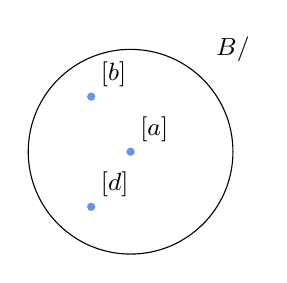
\begin{tikzpicture}[x=10mm,y=10mm, font=\small]
\draw (0,0) circle [x radius=1.3, y radius=1.3];

\node at (1.3,1.3) {$B/\Rel$};

\begin{scope}[fill=CornflowerBlue]
\fill  (0,0)circle (1.5pt) node[above right] {$[a]$};
\fill (-.5,.7) circle (1.5pt)node[above right] {$[b]$};
\fill(-.5,-.7) circle (1.5pt)node[above right] {$[d]$};
\end{scope}
\end{tikzpicture}

\end{center}


\osservazione Ogni volta che si ha una relazione d'equivalenza~$\Rel$ in un 
insieme~$A$, possiamo stabilire la seguente
catena di passaggi:
 \[\text{insieme }A\rightarrow\text{ partizione }P(A)\rightarrow\text{ insieme 
quoziente }A/\Rel.\]

% \ovalbox{\risolvii \ref{ese:B.32}, \ref{ese:B.33}, \ref{ese:B.34}, 
% \ref{ese:B.35}, \ref{ese:B.36}, \ref{ese:B.37}, \ref{ese:B.38}, \ref{ese:B.39}, 
% \ref{ese:B.40},
% \ref{ese:B.41}, \ref{ese:B.42}}

% \ovalbox{\ref{ese:B.43}}

\end{comment}

\subsection{Relazioni di ordine}
\label{subsec:rel_ordine}

Nel linguaggio di ogni giorno avrai certamente spesso usato espressioni come 
``devo mettere in ordine i miei
libri'' oppure ``qui non c'è ordine'' e altre espressioni simili.

Anche in matematica, fin dalla scuola elementare, hai imparato a ordinare gli 
elementi dell'insieme dei
numeri naturali: dati due numeri naturali hai imparato infatti a stabilire quale 
dei due è il maggiore.

\begin{definizione}
Una relazione~$\Rel$, introdotta in un insieme~$A$, si chiama \emph{relazione 
d'ordine} se è antisimmetrica e transitiva.
\end{definizione}

Riguardando le varie relazioni introdotte sin qui, possiamo stabilire che 
esistono relazioni d'ordine di vario tipo, schematizzate nel seguente diagramma:
\begin{center}
 % (c) 2012 Dimitrios Vrettos - d.vrettos@gmail.com

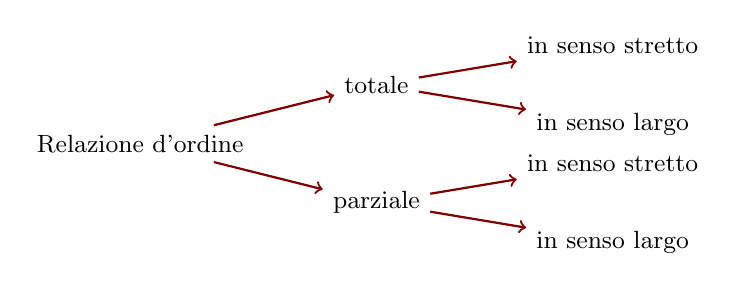
\begin{tikzpicture}[x=10mm,y=10mm, font=\small]

\node {Relazione d'ordine}[grow=right,level distance= 30mm, sibling distance=15mm,->,thick, draw=Maroon]
child {node {parziale}[sibling distance=10mm]
child {node {in senso largo}}
child {node {in senso stretto}}}
child {node {totale}[sibling distance=10mm]
child {node {in senso largo}}
child {node {in senso stretto}}};

\end{tikzpicture}

\end{center}

Attraverso alcuni esempi, vogliamo chiarire le differenze tra i diversi tipi; a 
questo scopo introduciamo la seguente definizione.

\begin{definizione}
Data una relazione~$\Rel$ d'ordine in un insieme~$A$, due elementi distinti~$x$ 
e~$y$ sono \emph{confrontabili} se rispetto ad~$\Rel$ si ha~$x R y$ oppure~$y R 
x$.
\end{definizione}

\begin{comment}
 
\begin{exrig}
 \begin{esempio}

In base al diagramma di Eulero-Venn nella figura~\ref{fig:B.5} introduciamo 
nell'insieme di insiemi~$S = \lbrace U, A, B, C, D, E, F \rbrace$ la 
relazione~$\Rel$: ``essere sottoinsieme di''.

Ricordiamo che, dati due insiemi~$X$ e~$Y$, $X$ è \emph{sottoinsieme} di~$Y$ 
quando ogni elemento di~$X$ appartiene a~$Y$ in simboli~$X \subseteq Y$ e
si legge~$X$ è contenuto in~$Y$ o~$X$ è uguale a~$Y$.

Vogliamo studiare le proprietà della relazione~$\Rel$:

\begin{enumeratea}
\item poiché ogni insieme è sottoinsieme di se stesso, possiamo dire che~$\Rel$ 
è riflessiva;
\item se~$X \subseteq Y$ e~$X \neq Y$ allora~$Y \not\subset X$ quindi~$\Rel$ è 
una relazione antisimmetrica;
\item se~$X \subseteq Y$ e~$Y \subseteq Z$ allora~$X \subseteq Z$ quindi~$\Rel$ 
è una relazione transitiva.
\end{enumeratea}

Inoltre è evidente che esistono almeno due elementi dell'insieme~$S$ che non 
sono in
alcun modo in relazione: ad esempio~$A \not\subset D$ e~$D \not\subset A$, 
ossia~$A$ e~$D$ non sono confrontabili.

 \end{esempio}

 \begin{esempio}

Riprendiamo il diagramma di Eulero-Venn dell'esempio precedente e introduciamo 
nell'insieme~$S = \lbrace U, A, B, C, D, E, F \rbrace$ la relazione~$\Rel$:
``essere sottoinsieme proprio di''. Studiamo le proprietà di questa relazione:
\begin{itemize*}
 \item cosa è cambiato rispetto alla relazione precedente? $\ldots$
 \item sono ancora valide le proprietà antisimmetrica e transitiva? $\ldots$
 \item esistono elementi di~$S$ non confrontabili? $\ldots$
\end{itemize*}

 \end{esempio}
\end{exrig}

\begin{definizione}
Una relazione d'ordine si dice \emph{parziale} quando almeno due elementi non 
sono confrontabili.
\end{definizione}

\begin{definizione}
Si dice relazione d'ordine parziale \emph{in senso largo} quando la relazione 
gode della proprietà riflessiva.
\end{definizione}

\begin{definizione}
Si dice relazione d'ordine parziale \emph{in senso stretto} quando la relazione 
gode della proprietà antiriflessiva.
\end{definizione}

\begin{definizione}
Una relazione d'ordine si dice \emph{totale} quando due qualsiasi elementi 
possono essre messi in relazione, cioè sono confrontabili.
\end{definizione}

\begin{definizione}
Si dice relazione d'ordine totale \emph{in senso largo} quando la relazione 
gode 
della proprietà riflessiva.
\end{definizione}

\begin{definizione}
Si dice relazione d'ordine totale \emph{in senso stretto} quando la relazione 
gode della proprietà antiriflessiva.
\end{definizione}

\begin{center}
 % (c) 2012 Dimitrios Vrettos - d.vrettos@gmail.com

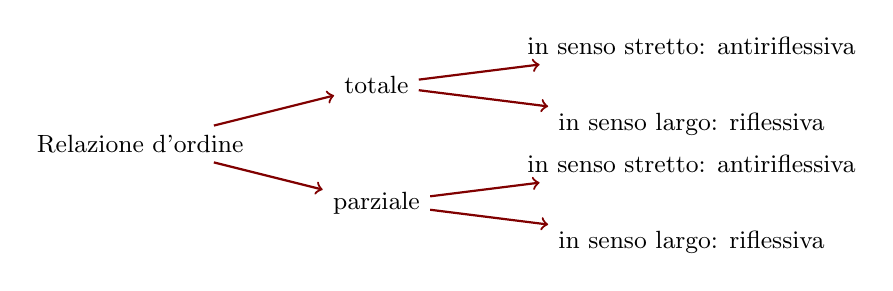
\begin{tikzpicture}[x=10mm,y=10mm, font=\small]

\node {Relazione d'ordine}[grow=right,level distance= 30mm,->,thick, draw=Maroon]
child {node {parziale}[level distance=40mm,sibling distance=10mm]
child {node {in senso largo: riflessiva}}
child {node {in senso stretto: antiriflessiva}}}
child {node {totale}[level distance=40mm,sibling distance=10mm]
child {node {in senso largo: riflessiva}}
child {node {in senso stretto: antiriflessiva}}};

\end{tikzpicture}

\end{center}

\end{comment}

% \ovalbox{\risolvii \ref{ese:B.44}, \ref{ese:B.45}, \ref{ese:B.46}, 
% \ref{ese:B.47}, \ref{ese:B.48}, \ref{ese:B.49}, \ref{ese:B.50}, \ref{ese:B.51},
% \ref{ese:B.52}, \ref{ese:B.53}, \ref{ese:B.54}}

% \ovalbox{ \ref{ese:B.55}, \ref{ese:B.56}, \ref{ese:B.57}, \ref{ese:B.58}, 
% \ref{ese:B.59}, \ref{ese:B.60},
% \ref{ese:B.61},\ref{ese:B.62}, \ref{ese:B.63}}


\section{Funzioni}
\label{sec:funzioni}

\subsection{Funzioni: definizioni}
\label{subsec:fun_definizioni}

Diamo la seguente definizione

\begin{definizione}
 Una corrispondenza univoca tra due insiemi~$A$ e~$B$ non vuoti
si chiama \emph{funzione o applicazione} di~$A$ in~$B$, se e solo se il dominio 
coincide con~$A: \Dom = \ID = A$.
\end{definizione}
In altre parole ogni elemento di $A$ è in corrispondenza con un solo elemento di 
$B$.
\begin{exrig}
 \begin{esempio}
\label{ex:D.1}
Analizziamo le corrispondenze rappresentate con grafico sagittale:
 \begin{center}
  % (c) 2012 Dimitrios Vrettos - d.vrettos@gmail.com
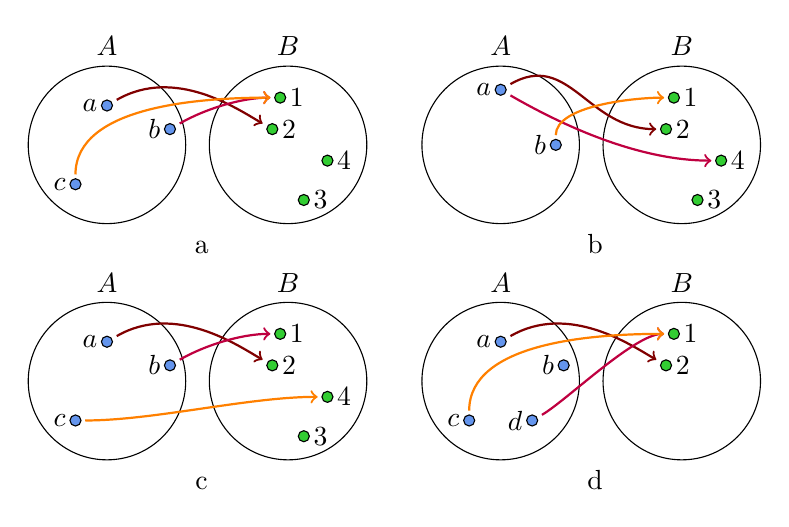
\begin{tikzpicture}[x=10mm, y=10mm]
%========================
% Prima coppia di insiemi
%========================
  \node[circle, minimum height=2cm,draw] (A) at (0,0) {};
  \node[above] (A1) at (A.north) {$A$};

  \begin{scope}[fill=CornflowerBlue]
    \filldraw (0,.5) circle (2pt) node (a) {};
    \node[left] at (0,.5) {$a$};
    \filldraw (.8,.2) circle (2pt) node (b) {};
    \node[left] at (.8,.2) {$b$};
    \filldraw (-.4,-.5) circle (2pt) node (c) {};
    \node[left] at (-.4,-.5)  {$c$};
  \end{scope}
  
  \node[anchor=south]  at (1.2,-1.5) {a};
  \begin{scope}[xshift=2.3cm]
  \node[circle, minimum height=2cm,draw] (B) at (0,0) {};
  \node[above] (B1) at (B.north) {$B$};

    \begin{scope}[fill=LimeGreen]
      \filldraw (-.1,.6) circle (2pt) node (a1) {};
      \filldraw (-.2,.2) circle (2pt)node (b1) {};
      \filldraw (.2,-.7) circle (2pt) node (c1) {};
      \filldraw(.5,-.2) circle (2pt);

      \node[right]  at (-.1,.6) {$1$};
      \node[right] at (-.2,.2) {$2$};
      \node[right]  at (.2,-.7) {$3$};
      \node[right] at (.5,-.2) {$4$};
    \end{scope}
  \end{scope}

  \begin{scope}[->,smooth,thick]
    \draw[Maroon] (a) .. controls +(30:1cm) and +(150:.5cm) .. (b1);
    \draw[purple] (b) .. controls +(30:.5cm) and +(180:0.5cm) .. (a1);
    \draw[orange] (c) .. controls +(90:1cm) and +(180:1cm) .. (a1);
  \end{scope}
%==========================
% Seconda coppia di insiemi
%==========================
  \begin{scope}[xshift=5cm]

  \node[circle, minimum height=2cm,draw] (A) at (0,0) {};
  \node[above] (A1) at (A.north) {$A$};
  \node [anchor=south] at (1.2,-1.5) {b};

  \begin{scope}[fill=CornflowerBlue]

      \filldraw (0,.7) circle (2pt) node (a) {};
      \node[left] at (0,.7) {$a$};
      \filldraw (.7,0) circle (2pt) node (b) {};
      \node[left] at (.7,0) {$b$};
    \end{scope}

    \begin{scope}[xshift=2.3cm]
      \node[circle, minimum height=2cm,draw] (B) at (0,0) {};
      \node[above] (B1) at (B.north) {$B$};

      \begin{scope}[fill=LimeGreen]
	\filldraw (-.1,.6) circle (2pt) node (a1) {};
	\filldraw (-.2,.2) circle (2pt)node (b1) {};
	\filldraw (.2,-.7) circle (2pt) node (c1) {};
	\filldraw(.5,-.2) circle (2pt) node (d1){};

	\node[right]  at (-.1,.6) {$1$};
	\node[right] at (-.2,.2) {$2$};
	\node[right]  at (.2,-.7) {$3$};
	\node[right] at (.5,-.2) {$4$};
      \end{scope}
    \end{scope}

    \begin{scope}[->,smooth,thick]
      \draw[Maroon] (a) .. controls +(30:1cm) and +(180:1cm) .. (b1);
      \draw[purple] (a) .. controls +(-30:1cm) and +(180:1cm) .. (d1);
      \draw[orange] (b) .. controls +(90:.5cm) and +(180:.5cm) .. (a1);
    \end{scope}
  \end{scope}
%========================
% Terza coppia di insiemi
%========================
  \begin{scope}[yshift=-3cm]
    \node[circle, minimum height=2cm,draw] (A) at (0,0) {};
    \node[above] (A1) at (A.north) {$A$};

    \begin{scope}[fill=CornflowerBlue]
      \filldraw (0,.5) circle (2pt) node (a) {};
      \node[left] at (0,.5) {$a$};
      \filldraw (.8,.2) circle (2pt) node (b) {};
      \node[left] at (.8,.2) {$b$};
      \filldraw (-.4,-.5) circle (2pt) node (c) {};
      \node[left] at (-.4,-.5)  {$c$};
    \end{scope}
    \node[anchor=south]  at (1.2,-1.5) {c};
    
    \begin{scope}[xshift=2.3cm]
      \node[circle, minimum height=2cm,draw] (B) at (0,0) {};
      \node[above] (B1) at (B.north) {$B$};
      
      \begin{scope}[fill=LimeGreen]
      \filldraw (-.1,.6) circle (2pt) node (a1) {};
      \filldraw (-.2,.2) circle (2pt)node (b1) {};
      \filldraw (.2,-.7) circle (2pt) node (c1) {};
      \filldraw(.5,-.2) circle (2pt) node(d1){};

      \node[right]  at (-.1,.6) {$1$};
      \node[right] at (-.2,.2) {$2$};
      \node[right]  at (.2,-.7) {$3$};
      \node[right] at (.5,-.2) {$4$};
      \end{scope}
    \end{scope}

    \begin{scope}[->,smooth,thick]
      \draw[Maroon] (a) .. controls +(30:1cm) and +(150:.5cm) .. (b1);
      \draw[purple] (b) .. controls +(30:.5cm) and +(180:0.5cm) .. (a1);
      \draw[orange] (c) .. controls +(0:1cm) and +(180:1cm) .. (d1);
    \end{scope}
  \end{scope}
%=========================  
% Quarta coppia di insiemi
%=========================  
  \begin{scope}[xshift=5cm,yshift=-3cm]
    \node[circle, minimum height=2cm,draw] (A) at (0,0) {};
    \node[above] (A1) at (A.north) {$A$};

    \begin{scope}[fill=CornflowerBlue]
      \filldraw (0,.5) circle (2pt) node (a) {};
      \node[left] at (0,.5) {$a$};
      \filldraw (.8,.2) circle (2pt) node (b) {};
      \node[left] at (.8,.2) {$b$};
      \filldraw (-.4,-.5) circle (2pt) node (c) {};
      \node[left] at (-.4,-.5)  {$c$};
      \filldraw (.4,-.5) circle (2pt) node (d) {};
      \node[left] at (.4,-.5)  {$d$};
    \end{scope}
    
    \node[anchor=south]  at (1.2,-1.5) {d};
    
    \begin{scope}[xshift=2.3cm]
    \node[circle, minimum height=2cm,draw] (B) at (0,0) {};
    \node[above] (B1) at (B.north) {$B$};

      \begin{scope}[fill=LimeGreen]
	\filldraw (-.1,.6) circle (2pt) node (a1) {};
	\filldraw (-.2,.2) circle (2pt)node (b1) {};

	\node[right]  at (-.1,.6) {$1$};
	\node[right] at (-.2,.2) {$2$};
      \end{scope}
    \end{scope}

    \begin{scope}[->,smooth,thick]
      \draw[Maroon] (a) .. controls +(30:1cm) and +(150:.5cm) .. (b1);
      \draw[purple] (d) .. controls +(30:.5cm) and +(180:0.5cm) .. (a1);
      \draw[orange] (c) .. controls +(90:1cm) and +(180:1cm) .. (a1);
    \end{scope}
  \end{scope}
\end{tikzpicture}

 \end{center}

La corrispondenza di figura~a rappresenta una funzione.

La corrispondenza di figura~b non rappresenta una funzione perché
l'elemento~$a$ di~$A$ è in corrispondenza con due
elementi di~$B$, il~2 e il~4, quindi non è una corrispondenza univoca.

La corrispondenza della figura~c rappresenta una funzione.

La corrispondenza della figura~d non è una funzione perché il
dominio non coincide con l'insieme~$A$.
 \end{esempio}

\end{exrig}

I termini funzione o applicazione sono sinonimi, tuttavia si preferisce
usare il termine ``funzione'' quando i due insiemi~$A$ e~$B$ sono insiemi 
numerici. Solitamente una funzione
viene indicata con la lettera~$f$ e si intende la legge
che \emph{associa ad ogni elemento~$x$ di~$A$ uno e uno solo elemento~$y$ 
di~$B$}.

Per indicare la legge che fa passare dall'insieme~$A$ all'insieme~$B$ usiamo la 
scrittura
\begin{equation*}
f:A \rightarrow B,\text{ oppure } A\overset{{f}}{{\rightarrow }}B
\end{equation*}

\begin{definizione}
 L'elemento~$y$ di~$B$, corrispondente di un elemento~$x$ del dominio, viene 
detto \emph{immagine di~$x$ nella funzione~$f$} e
si scrive~$y = f(x)$ che si legge \emph{``$y$ uguale effe di~$x$''}.
\end{definizione}


Il sottoinsieme proprio o improprio di~$B$ formato dagli elementi che sono
immagini degli elementi del dominio si chiama
\emph{codominio o insieme immagine} e si scrive~$\Cod = \IM = f(\Dom)$. 
Osserviamo che non necessariamente
ogni elemento di~$B$ è immagine di un elemento del dominio per 
cui~$\Cod\subseteq B$.

%  \vspazio\ovalbox{\risolvii \ref{ese:D.1}, \ref{ese:D.2}, \ref{ese:D.3}, 
% \ref{ese:D.4}}

\subsubsection{Funzioni iniettive, suriettive, biiettive}

\begin{exrig}
 \begin{esempio}
Nella figure sottostanti sono rappresentate alcune funzioni:
\begin{center}
 % (c) 2012 Dimitrios Vrettos - d.vrettos@gmail.com
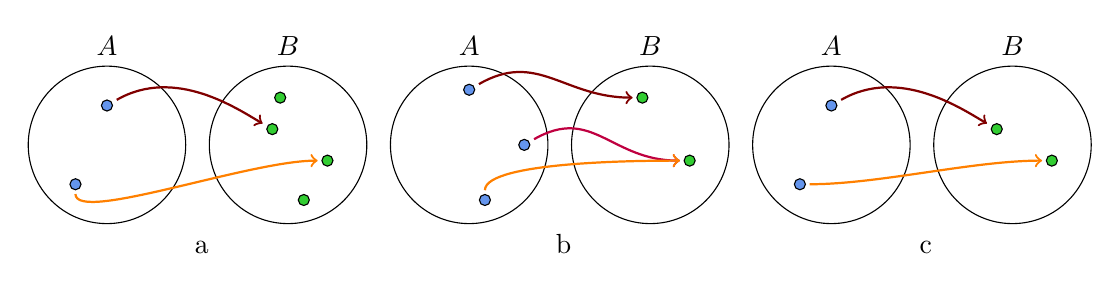
\begin{tikzpicture}[x=10mm, y=10mm]

  \node[circle, minimum height=2cm,draw] (A) at (0,0) {};
  \node[above] (A1) at (A.north) {$A$};

  \begin{scope}[fill=CornflowerBlue]
    \filldraw (0,.5) circle (2pt) node (a) {};
    \filldraw (-.4,-.5) circle (2pt) node (c) {};
    \node[left] at (-.4,-.5)  {};
  \end{scope}
  
  \node[anchor=south]  at (1.2,-1.5) {a};
  \begin{scope}[xshift=2.3cm]
    \node[circle, minimum height=2cm,draw] (B) at (0,0) {};
    \node[above] (B1) at (B.north) {$B$};
    
    \begin{scope}[fill=LimeGreen]
      \filldraw (-.1,.6) circle (2pt) node (a1) {};
      \filldraw (-.2,.2) circle (2pt)node (b1) {};
      \filldraw (.2,-.7) circle (2pt) node (c1) {};
      \filldraw(.5,-.2) circle (2pt) node(d1) {};
    \end{scope}
  \end{scope}

  \begin{scope}[->,smooth,thick]
    \draw[Maroon] (a) .. controls +(30:1cm) and +(150:.5cm) .. (b1);
    \draw[orange] (c) .. controls +(-90:.5cm) and +(180:1cm) .. (d1);
  \end{scope}

  \begin{scope}[xshift=4.6cm]
    \node[circle, minimum height=2cm,draw] (A) at (0,0) {};
    \node[above] (A1) at (A.north) {$A$};
    \node [anchor=south] at (1.2,-1.5) {b};
    \begin{scope}[fill=CornflowerBlue]

      \filldraw (0,.7) circle (2pt) node (a) {};
      \filldraw (.7,0) circle (2pt) node (b) {};
      \filldraw (.2,-.7) circle (2pt) node (c) {};
    \end{scope}

    \begin{scope}[xshift=2.3cm]
    \node[circle, minimum height=2cm,draw] (B) at (0,0) {};

    \node[above] (B1) at (B.north) {$B$};

      \begin{scope}[fill=LimeGreen]
	\filldraw (-.1,.6) circle (2pt) node (a1) {};
	\filldraw(.5,-.2) circle (2pt) node (d1){};
      \end{scope}
    \end{scope}

    \begin{scope}[->,smooth,thick]
      \draw[Maroon] (a) .. controls +(30:1cm) and +(180:1cm) .. (a1);
      \draw[purple] (b) .. controls +(30:1cm) and +(180:1cm) .. (d1);
      \draw[orange] (c) .. controls +(90:.5cm) and +(180:.5cm) .. (d1);
    \end{scope}
  \end{scope}

  \begin{scope}[xshift=9.2cm]
    \node[circle, minimum height=2cm,draw] (A) at (0,0) {};
    \node[above] (A1) at (A.north) {$A$};

    \begin{scope}[fill=CornflowerBlue]
      \filldraw (0,.5) circle (2pt) node (a) {};
      \filldraw (-.4,-.5) circle (2pt) node (c) {};
    \end{scope}
    \node[anchor=south]  at (1.2,-1.5) {c};
  
    \begin{scope}[xshift=2.3cm]
      \node[circle, minimum height=2cm,draw] (B) at (0,0) {};
      \node[above] (B1) at (B.north) {$B$};

      \begin{scope}[fill=LimeGreen]
	\filldraw (-.2,.2) circle (2pt)node (b1) {};
	\filldraw(.5,-.2) circle (2pt) node(d1){};
      \end{scope}
    \end{scope}

    \begin{scope}[->,smooth,thick]
      \draw[Maroon] (a) .. controls +(30:1cm) and +(150:.5cm) .. (b1);
      \draw[orange] (c) .. controls +(0:1cm) and +(180:1cm) .. (d1);
    \end{scope}
  \end{scope}
\end{tikzpicture}
\end{center}

In figura~a si ha~$\IM\subset B$ elementi distinti del dominio~$A$ hanno 
immagini distinte in~$B$.

In figura~b si ha~$\IM=B$ ma elementi distinti di~$A$ hanno la stessa immagine 
in~$B$.

In figura~b si ha~$\IM=B$ ed elementi distinti del dominio~$A$ hanno immagini 
distinte in~$B$.
 \end{esempio}
\end{exrig}

I tre esempi illustrano tre tipi diversi di funzioni:

\begin{definizione}
Si dice \emph{iniettiva} una funzione per la quale elementi distinti del
dominio hanno immagini distinte in~$B$: per \emph{qualunque}~$x_1$, $x_2$ di~$A$
con~$x_1\neq x_2$, si ha~$f(x_1)\neq f(x_2)$.
\end{definizione}

\begin{definizione}
Si dice \emph{suriettiva} una funzione in cui~$\IM = B$.
\end{definizione}

\begin{definizione}
Si dice \emph{biunivoca o biiettiva} una funzione che sia
\emph{contemporaneamente iniettiva e suriettiva.}
\end{definizione}

Pertanto in figura~a è rappresentata una funzione iniettiva, in figura~b una
funzione suriettiva e in figura~c una funzione biunivoca.

%  \vspazio\ovalbox{\risolvii \ref{ese:D.5}, \ref{ese:D.6}}
%  \newpage
\subsubsection{Diagramma riepilogativo sui diversi tipi di corrispondenze}

\begin{center}
 % (c) 2012 Dimitrios Vrettos - d.vrettos@gmail.com
\begin{tikzpicture}[x=10mm, y=10mm,filled/.style={fill=circle area, thick}]
\draw (0,0) rectangle (5,4) node[above right] {$C$};
  \node[ellipse, minimum height=3cm, minimum width=4.5cm,draw=blue,thick] (F) at (2.5,2) {};
  \node[above, blue] (F1) at (F.north) {$F$};

\def\firstcircle{(1.7,1.9) circle (1cm)}
\def\secondcircle{(2.9,1.9) circle (1.25cm)}
\definecolor{circle area}{gray}{0.9}
    \begin{scope}
        \clip \firstcircle;
        \fill[filled] \secondcircle;
    \end{scope}
    \draw[OliveGreen, thick]\firstcircle;
    \draw[Maroon,thick] \secondcircle;
    \node[OliveGreen] at (1.1,1.9) {$I$};
	\node[Maroon] at (3.1,1.9) {$S$};

\begin{scope}[xshift=6cm, yshift=2cm]
\matrix[matrix of nodes, right,column 1/.style={anchor=base west,},
column 2/.style={anchor=base west}, column sep=.5cm
]{
Legenda&\\
$C$& insieme delle corrispondenze\\
|[blue]|$F$&insieme delle funzioni\\
|[Maroon]|$S$&insieme delle funzioni suriettive\\
|[OliveGreen]|$I$&insieme delle funzioni iniettive\\
$I \cap S$&insieme delle funzioni biunivoche\\};
\end{scope}
\end{tikzpicture}
\end{center}

\begin{comment}
 
\subsection{Funzioni tra insiemi numerici}
\label{subsec:fun_numeriche}

Analizziamo alcune corrispondenze definite tra gli insiemi numerici. In
questo caso la funzione~$f$ può essere espressa
tramite una formula o scrittura analitica, una tabella, un algoritmo,
oppure semplicemente con linguaggio comune, purché in modo preciso e
inequivocabile. Il generico elemento~$x$ del dominio si chiama
\emph{variabile indipendente}; il corrispondente elemento~$y =f(x)$ si chiama 
\emph{variabile dipendente}.

\begin{exrig}
 \begin{esempio}
 \label{ex:D.3}
Consideriamo la corrispondenza~$\Kor$: ``essere il valore assoluto di'' tra
l'insieme~$\insN_0$ dei naturali diversi da zero e l'insieme~$\insZ_0$ degli 
interi
relativi diversi da zero. Questa corrispondenza \emph{non è una
funzione} in quanto \emph{non è} una corrispondenza \emph{univoca}: un elemento 
di~$\insN_0$ ha due immagini
poiché ogni numero naturale è valore assoluto di due interi
opposti, come rappresentato dalla figura~\ref{fig:D.1}.
\end{esempio}

\begin{inaccessibleblock}[Figura: TODO]
 \begin{figure}[b]
 \begin{minipage}[t]{.45\textwidth}
\centering
 % (c) 2012 Dimitrios Vrettos - d.vrettos@gmail.com
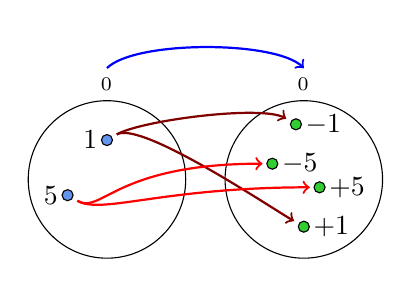
\begin{tikzpicture}[x=10mm, y=10mm]

\node[circle, minimum height=2cm,draw] (D) at (0,0) {};

\node[above] (D1) at (D.north) {$\insN_0$};
\begin{scope}[fill=CornflowerBlue]

\filldraw (0,.5) circle (2pt) node (a) {};
\node[left] at (0,.5) {1};
\filldraw (-.5,-.2) circle (2pt) node (d) {};
\node[left] at (-.5,-.2) {5};
\end{scope}

\begin{scope}[xshift=2.5cm]
\node[circle, minimum height=2cm,draw] (C) at (0,0) {};

\node[above] (C1) at (C.north) {$\insZ_0$};

\begin{scope}[fill=LimeGreen]
\filldraw (-.1,.7) circle (2pt) node (a1) {};
\filldraw (-.4,.2) circle (2pt)node (b1) {};
\filldraw (0,-.6) circle (2pt) node (c1) {};
\filldraw (.2,-.1) circle (2pt) node (d1) {};
\node[right]  at (-.1,.7) {$-1$};
\node[right]  at (0,-.6) {$+1$};
\node[right] at (-.4,.2) {$-5$};
\node[right] at (.2,-.1) {$+5$};
\end{scope}
\end{scope}
\begin{scope}[->,smooth,thick]
\draw[blue] (D1.north) .. controls +(45:.5cm) and +(135:.5cm) .. (C1.north) node [midway, above, black] () {$\Kor$};
\draw[Maroon] (a) .. controls +(30:.5cm) and +(150:.5cm) .. (c1);
 \draw[Maroon] (a) .. controls +(30:.5cm) and +(150:.5cm) .. (a1);
\draw[red] (d) .. controls +(-30:.5cm) and +(-180:2cm) .. (b1);
\draw[red] (d) .. controls +(-30:.5cm) and +(-180:2cm) .. (d1);
\end{scope}
\end{tikzpicture}

\caption{Esempio~\ref{ex:D.3}.}\label{fig:D.1}
 \end{minipage}\hfil
 \begin{minipage}[t]{.45\textwidth}
\centering
 % (c) 2012 Dimitrios Vrettos - d.vrettos@gmail.com
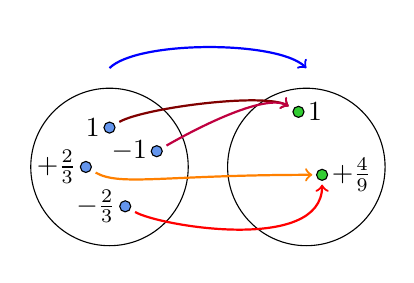
\begin{tikzpicture}[x=10mm, y=10mm]

\node[circle, minimum height=2cm,draw] (D) at (0,0) {};

\node[above] (D1) at (D.north) {$\insQ$};
\begin{scope}[fill=CornflowerBlue]

\filldraw (0,.5) circle (2pt) node (a) {};
\node[left] at (0,.5) {1};
\filldraw (0.6,.2) circle (2pt) node (b) {};
\node[left] at (0.6,.2) {$-1$};
\filldraw (.2,-.5) circle (2pt) node (c) {};
\node[left] at (.2,-.5) {$-\frac{2}{3}$};
\filldraw (-.3,0) circle (2pt) node (d) {};
\node[left] at (-.3,0) {$+\frac{2}{3}$};
\end{scope}

\begin{scope}[xshift=2.5cm]
\node[circle, minimum height=2cm,draw] (C) at (0,0) {};

\node[above] (C1) at (C.north) {$\insQ$};

\begin{scope}[fill=LimeGreen]
\filldraw (-.1,.7) circle (2pt) node (a1) {};
\filldraw (.2,-.1) circle (2pt) node (d1) {};
\node[right]  at (-.1,.7) {$1$};
\node[right] at (.2,-.1) {$+\frac{4}{9}$};
\end{scope}
\end{scope}
\begin{scope}[->,smooth,thick]
\draw[blue] (D1.north) .. controls +(45:.5cm) and +(135:.5cm) .. (C1.north) node [midway, above, black] () {$\Kor$};
\draw[Maroon] (a) .. controls +(30:.5cm) and +(150:.5cm) .. (a1);
 \draw[purple] (b) .. controls +(30:.5cm) and +(150:.5cm) .. (a1);
\draw[red] (c) .. controls +(-30:.5cm) and +(-90:1cm) .. (d1);
\draw[orange] (d) .. controls +(-30:.5cm) and +(-180:2cm) .. (d1);
\end{scope}
\end{tikzpicture}
\caption{Esempio~\ref{ex:D.4}.}\label{fig:D.2}
 \end{minipage}
\end{figure}
\end{inaccessibleblock}

 \begin{esempio}
 \label{ex:D.4}
 Consideriamo la corrispondenza~$\Kor$ che \emph{associa ad ogni numero 
razionale il suo quadrato}. Essa è una funzione di
dominio~$\insQ$: di ogni numero razionale si può
determinare il quadrato che è unico; poiché numeri opposti hanno lo
stesso quadrato la funzione in esame \emph{non} è
\emph{iniettiva}, come rappresentato dalla figura~\ref{fig:D.2}.

L'immagine~$y$ di ogni~$x$ appartenente a~$\insQ$ è il suo
quadrato: in simboli matematici scriviamo la funzione tramite una
formula~$f: y = x^{2}$.

Per quanto riguarda l'insieme immagine o
codominio della funzione esso è un sottoinsieme proprio di~$\insQ$: il numero 
razionale~$+{\frac{3}{4}}$ non è quadrato di
nessun razionale e neppure~$-25$, razionale negativo, è quadrato di
un numero razionale, quindi~$\IM\subset\insQ^{+}\cup\{0\}$, pertanto la funzione 
non è suriettiva.
 \end{esempio}

 \begin{esempio}
 \label{ex:D.5}
 Analizziamo la corrispondenza che associa \emph{ad ogni intero} il suo valore 
assoluto.

Sappiamo che il valore assoluto di un intero è un numero naturale, e
ogni intero ha un solo valore assoluto. La corrispondenza è univoca e
il dominio coincide con l'insieme~$\insZ$, pertanto è una
funzione:~$f: \insZ\rightarrow\insN$ rappresentata in forma
analitica con~${y=\valass{x}}$ con~$x\in\insZ$ e~$y=f(x)\in\insN$.

\begin{center}
\begin{tabular}{l*8{c}}
 \toprule
$x\in \insZ$ & 0 & $+1$ & $-1$ & $-2$ & $+2$ & $+3$ & $-3$ & \ldots\\
$y\in \insN$ & 0 & 1 & 1 & 2 & 2 & 3 & 3 & \ldots \\
\bottomrule
\end{tabular}
\end{center}
Nella tabella sono rappresentati alcuni elementi del dominio
con le rispettive immagini: da cui si deduce che tale funzione non è
iniettiva.
 \end{esempio}

 \begin{esempio}
 \label{ex:D.6}
È assegnata la funzione~$f:x\in N\rightarrow (x-2)\in\insZ$. In questo caso la 
funzione associa ad ogni numero naturale $x$ il
numero intero ottenuto sottraendo~2 da $x$. L'espressione analitica della 
funzione è~$f: y = x-2$. La legge così espressa si può descrivere anche 
attraverso una
tabella.

\begin{center}
\begin{tabular}{l*8{c}}
 \toprule
$x\in \insN$ & 0 & 1 & 2 & 3 & 4 & 5 & 6 & \ldots \\
$(x-2)\in \insZ$ & $-2$ & $-1$ & 0 & $+1$ & $+2$ & $+3$ & $+4$ & \ldots \\
\bottomrule
\end{tabular}
\end{center}

Ogni elemento dell'insieme~$\insN$ trova il corrispondente in~$\insZ$ elementi 
diversi del dominio hanno immagini diverse pertanto la
funzione è \emph{iniettiva}; il codominio o insieme immagine è un sottoinsieme 
proprio di~$\insZ$ e precisamente~$\Cod = IM =\{y\in\insZ/y\geqslant -2\}$,
pertanto la funzione non è suriettiva.
 \end{esempio}

 \begin{esempio}
 \label{ex:D.7}
 Analizziamo la corrispondenza:~$f_{1}:x\in \insN\rightarrow (x-2)\in N$ e 
costruiamo la relativa tabella:

Vediamo che nella corrispondenza assegnata né~0 né~1 hanno l'immagine.

\begin{center}
\begin{tabular}{l*8{c}}
\toprule
$x\in \insN$ & 0 & 1 & 2 & 3 & 4 & 5 & 6 & \ldots \\
$(x-2)\in \insN$ & & & 0 & 1 & 2 & 3 & 4 & \ldots \\
\bottomrule
\end{tabular}
\end{center}

Fissiamo allora come dominio un sottoinsieme di~$\insN$ e precisamente~$\Dom = 
\ID = \insN - \{0,1\}$,
in questo modo possiamo procedere nell'analisi della funzione~$f_{1}:y=x-2$.
\end{esempio}

 \begin{esempio}
 Consideriamo la corrispondenza che associa ad ogni numero razionale il suo 
inverso (o reciproco).

Sappiamo che ``fare l'inverso'' di un numero razionale~$x$
significa scrivere il numero razionale~$\frac{1}{x}$, ma questa
operazione ha significato solo se~$x$ è diverso da~0; operiamo dunque
una restrizione su $\insQ$ e fissiamo~$\Dom = \ID = \insQ_0$. La corrispondenza 
è una funzione tra~$\insQ_0$
e~$\insQ$. In simboli matematici~$f: y=\frac{1}{x}$.
 \end{esempio}
\end{exrig}


% \ovalbox{\risolvii \ref{ese:D.7}, \ref{ese:D.8}, \ref{ese:D.9}, 
% \ref{ese:D.10}, \ref{ese:D.11}}

\subsection{Funzioni inverse}
\label{subsec:fun_inverse}

È assegnata la funzione~$f:\insR\rightarrow \insR$ descritta mediante le 
istruzioni
\begin{center}
 % (c) 2012 Dimitrios Vrettos - d.vrettos@gmail.com
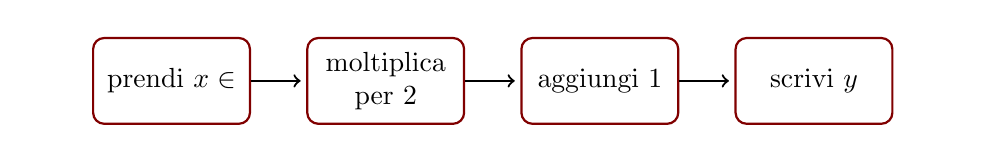
\begin{tikzpicture}
[auto,block/.style
={rectangle, draw=Maroon, thick,
text width=5em,align=center, rounded corners,
minimum height=3.1em},
line/.style
={draw, thick, ->,shorten >=2pt}]
\matrix [column sep=7mm]{
& \node [block] (prn) {prendi $x\in \insR$}; 
& \node [block] (molt) {moltiplica per 2}; 
& \node [block] (agg) {aggiungi 1}; 
& \node [block] (scr) {scrivi $y$}; & \\
};
\begin{scope}[every path/.style=line]
\path (prn)-- (molt);
\path (molt) -- (agg);
\path (agg)--(scr);
\end{scope}
\end{tikzpicture}
\end{center}

La forma algebrica è~$y=2\cdot x+1$ essa è definita per qualunque
numero reale e l'insieme immagine coincide con il codominio.

Scelto arbitrariamente un valore per la variabile
indipendente come~$x=-2$ otteniamo la sua immagine~$y=-3$, risultato
delle operazioni descritte nelle istruzioni.

Preso ora~$y=4$, elemento dell'insieme immagine della
funzione, quali istruzioni dobbiamo seguire per determinarne la
controimmagine? Il problema si formalizza in questo modo:
``per quale valore di~$x$ aggiungendo~1 al suo doppio si
ottiene~4?''

Le due questioni sono rappresentate nel diagramma di Eulero-Venn 
(figura~\ref{fig:D.3}) e
percorrendo le istruzioni con le operazioni inverse otteniamo il valore di~$x$
sottraendo~1 al valore dato per~$y$ e dividendo il risultato per~2. Le
nuove istruzioni da eseguire sono:
\begin{center}
 % (c) 2012 Dimitrios Vrettos - d.vrettos@gmail.com
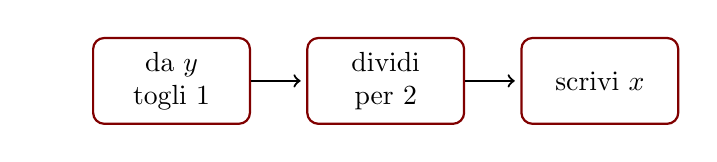
\begin{tikzpicture}
[auto,block/.style
={rectangle, draw=Maroon, thick,
text width=5em,align=center, rounded corners,
minimum height=3.1em},
line/.style
={draw, thick, ->,shorten >=2pt}]
\matrix [column sep=7mm]{
& \node [block] (prn) { da~$y$ togli 1}; 
& \node [block] (molt) {dividi per 2}; 
& \node [block] (agg) {scrivi~$x$}; \\
};
\begin{scope}[every path/.style=line]
\path (prn)-- (molt);
\path (molt) -- (agg);
\end{scope}
\end{tikzpicture}
\end{center}

In formula~$x=(y-1):2$.

La funzione così ottenuta si chiama \emph{funzione inversa} di~$f(x)$
e si scrive~$f^{-1}$.

Poiché la funzione assegnata è iniettiva, ci rendiamo subito conto
che per ogni~$y$ dell'insieme immagine possiamo
determinare la controimmagine (cioè l'unico valore di~$x$ tale che~$f(x) = y$).

\begin{inaccessibleblock}[Figura: TODO]
 \begin{figure}[b]
\centering% (c) 2012 Dimitrios Vrettos - d.vrettos@gmail.com
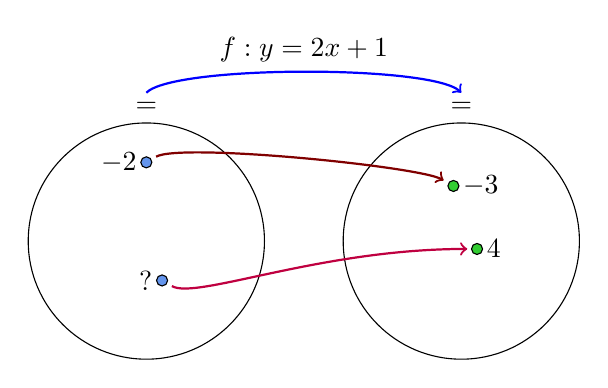
\begin{tikzpicture}[x=10mm, y=10mm]

\node[circle, minimum height=3cm,draw] (D) at (0,0) {};

\node[above] (D1) at (D.north) {$\Dom=\insR$};
\begin{scope}[fill=CornflowerBlue]

\filldraw (0,1) circle (2pt) node (a) {};
\node[left] at (0,1) {$-2$};

\filldraw (.2,-.5) circle (2pt) node (c) {};
\node[left] at (.2,-.5) {?};

\end{scope}

\begin{scope}[xshift=4cm]
\node[circle, minimum height=3cm,draw] (C) at (0,0) {};

\node[above] (C1) at (C.north) {$\Cod=\insR$};

\begin{scope}[fill=LimeGreen]
\filldraw (-.1,.7) circle (2pt) node (a1) {};
\filldraw (.2,-.1) circle (2pt) node (d1) {};
\node[right]  at (-.1,.7) {$-3$};
\node[right] at (.2,-.1) {$4$};
\end{scope}
\end{scope}
\begin{scope}[->,smooth,thick]
\draw[blue] (D1.north) .. controls +(45:.5cm) and +(135:.5cm) .. (C1.north) node [midway, above, black] () {$f:y=2x+1$};
\draw[Maroon] (a) .. controls +(30:.5cm) and +(150:.5cm) .. (a1);
\draw[purple] (c) .. controls +(-30:.5cm) and +(-180:2cm) .. (d1);
\end{scope}
\end{tikzpicture}
\caption{Funzioni inverse.}\label{fig:D.3}
\end{figure}
\end{inaccessibleblock}

\begin{definizione}
Per \emph{funzione inversa} di una funzione iniettiva~$y = f(x)$ si intende 
quella funzione che permette di determinare la
controimmagine di un qualunque elemento dell'insieme immagine di~$f(x)$. Il 
simbolo della funzione inversa è~$f^{-1}$.
\end{definizione}

Osserviamo che~$\Dom\left(f^{-1}\right)=\IM(f)$ 
e~$\IM\left(f^{-1}\right)=\Dom(f)$.

% \vspazio\ovalbox{\risolvii \ref{ese:D.12}, \ref{ese:D.13}}

\subsection{Funzioni composte}
\label{subsec:fun_composte}

Date due funzioni~$f:A\rightarrow B$ e~$g:B\rightarrow C$ è
possibile definire la funzione composta
\[g\circ f:A\rightarrow C\]
che a un elemento~$a$ di~$A$ associa prima l'elemento~$b=f(a)$ e
poi l'elemento~$c=g(b)$, in un'unica
formula si può scrivere~$g(f(a))=c$.
\begin{center}
 % (c) 2012 Dimitrios Vrettos - d.vrettos@gmail.com
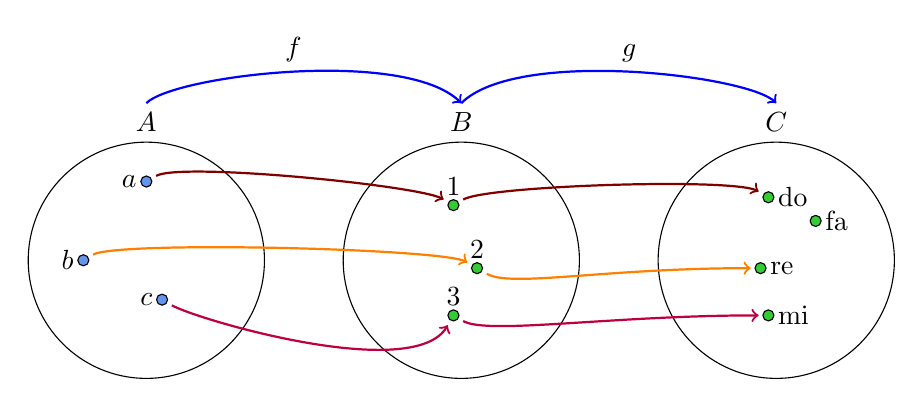
\begin{tikzpicture}[x=10mm, y=10mm]

\node[circle, minimum height=3cm,draw] (A) at (0,0) {};

\node[above] (A1) at (A.north) {$A$};
\begin{scope}[fill=CornflowerBlue]

\filldraw (0,1) circle (2pt) node (a) {};
\node[left] at (0,1) {$a$};
\filldraw (-.8,0) circle (2pt) node (b) {};
\node[left] at (-.8,0) {$b$};
\filldraw (.2,-.5) circle (2pt) node (c) {};
\node[left] at (.2,-.5) {$c$};

\end{scope}

\begin{scope}[xshift=4cm]
\node[circle, minimum height=3cm,draw] (B) at (0,0) {};

\node[above] (B1) at (B.north) {$B$};

\begin{scope}[fill=LimeGreen]
\filldraw (-.1,.7) circle (2pt) node (a1) {};
\filldraw (-.1,-.7) circle (2pt) node (c1) {};
\filldraw (.2,-.1) circle (2pt) node (b1) {};
\node[above]  at (-.1,.7) {$1$};
\node[above] at (.2,-.1) {$2$};
\node[above]  at (-.1,-.7) {$3$};
\end{scope}
\end{scope}
\begin{scope}[->,smooth,thick]
\draw[blue] (A1.north) .. controls +(45:.5cm) and +(135:1cm) .. (B1.north) node [midway, above, black] () {$f$};
\draw[Maroon] (a) .. controls +(30:.5cm) and +(150:.5cm) .. (a1);
\draw[orange] (b) .. controls +(30:.5cm) and +(150:.5cm) .. (b1);
\draw[purple] (c) .. controls +(-30:.5cm) and +(-120:1cm) .. (c1);
\end{scope}

\begin{scope}[xshift=8cm]
\node[circle, minimum height=3cm,draw] (C) at (0,0) {};

\node[above] (C1) at (C.north) {$C$};

\begin{scope}[fill=LimeGreen]
\filldraw (-.1,.8) circle (2pt) node (a2) {};
\filldraw (-.1,-.7) circle (2pt) node (c2) {};
\filldraw (-.2,-.1) circle (2pt) node (b2) {};
\filldraw (.5,.5) circle (2pt) node (d2) {};
\node[right]  at (-.1,.8) {do};
\node[right] at (-.2,-.1) {re};
\node[right]  at (-.1,-.7) {mi};
\node[right]  at (.5,.5) {fa};
\end{scope}
\end{scope}
\begin{scope}[->,smooth,thick]
 \draw[blue] (B1.north) .. controls +(45:1cm) and +(135:.5cm) .. (C1.north) node [midway, above, black] () {$g$};
\draw[Maroon] (a1) .. controls +(30:.5cm) and +(150:.5cm) .. (a2);
\draw[orange] (b1) .. controls +(-30:.5cm) and +(-180:2cm) .. (b2);
\draw[purple] (c1) .. controls +(-30:.5cm) and +(-180:2cm) .. (c2);
\end{scope}
\end{tikzpicture}
\end{center}

\begin{exrig}
 \begin{esempio}
 Data la funzione~$f(x)=2x$ e la funzione~$g(x)=x+1$, determina
l'espressione analitica della funzione composta.

Prima agisce la funzione~$f$ che raddoppia il valore di~$x$. Al valore
ottenuto, che è~$2x$, si applica la~$g$ che fa aumentare di~1. Pertanto
la funzione composta raddoppia~$x$ e poi aggiunge~1.
L'espressione è~$g(f(x))=2x+1$.
 \end{esempio}

\end{exrig}

Osserva che la composizione di funzioni non è commutativa. Infatti la
funzione~$f(g(x))$ si ottiene facendo agire prima la~$g(x)$ che aumenta di~1
il valore della variabile e poi la~$f(x)$ che raddoppia il valore della
variabile; allora~$f(g(x))=2(x+1)$.

% \vspazio\ovalbox{\risolvi \ref{ese:D.14}}

\subsection{La retta e gli insiemi numerici}
\label{subsec:fun_retta}

Nello studio degli insiemi numerici abbiamo visto come si possono depositare su 
una semiretta i numeri naturali;
la legge costruttiva di questa rappresentazione genera tra 
l'insieme~$\insN=\{0,1,2,3,4,\ldots \}$ e i punti della
semiretta una corrispondenza avente come dominio~$\insN$ e come codominio i 
punti della semiretta.
Ad ogni numero naturale possiamo far corrispondere un punto della semiretta, ma 
\emph{non tutti i punti} della semiretta
\emph{sono immagine} di un numero naturale: la \emph{corrispondenza non è 
biunivoca}.

Lo stesso fatto avviene se consideriamo l'insieme~$\insZ$ come dominio e i punti 
di una retta orientata come codominio;
nella figura viene rappresentata la corrispondenza generata con la legge 
costruttiva già enunciata nel capitolo dei numeri interi.
\begin{center}
 % (c) 2012 Dimitrios Vrettos - d.vrettos@gmail.com
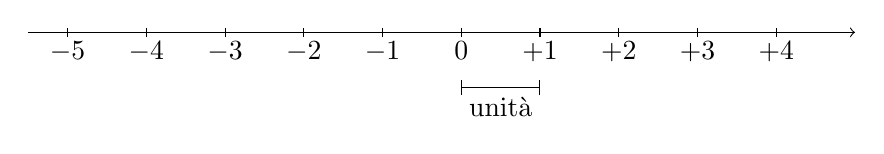
\begin{tikzpicture}[x=10mm, y=10mm]
\draw[->](-5.5,0) -- (5,0);
\foreach \x in {-5,-4,...,4}
\draw (\x,1.5pt) -- (\x,-1.5pt);

\draw[|-|] (0,-.7) -- (1,-.7) node [below, midway] () {unità};

\foreach \x/\xtext in {-5/-5,-4/-4,-3/-3,-2/-2,-1/-1,0/0,1/+1,2/+2,3/+3,4/+4}
\node[below] at (\x,0) {$\xtext$};
\end{tikzpicture}
\end{center}

Ad ogni numero intero possiamo far corrispondere un punto della retta orientata, 
ma \emph{non tutti i punti} della retta \emph{sono immagine}
di un numero intero: l'insieme immagine non coincide con il codominio e la 
\emph{corrispondenza non è biunivoca}.

Gli insiemi~$\insN$ e~$\insZ$ sono infiniti e la loro caratteristica comune è 
che tra due naturali consecutivi o tra due interi consecutivi
non possiamo trovarne un altro. Si dice che~$\insN$ e~$\insZ$ sono due 
\emph{insiemi discreti}.

Consideriamo ora l'insieme~$\insQ$ dei numeri razionali; sappiamo che anche 
questi numeri, rappresentati da frazioni, possono essere disposti
su una retta orientata come mostrato nella figura sottostante.
\begin{center}
 % (c) 2012 Dimitrios Vrettos - d.vrettos@gmail.com
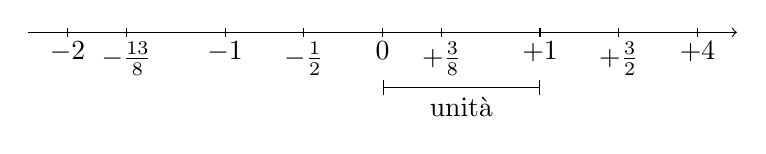
\begin{tikzpicture}[x=10mm, y=10mm]
\draw[->](-4.5,0) -- (4.5,0);
\foreach \x in {-4,-3.25,-2,-1,0,.75,2,3,4}
\draw (\x,1.5pt) -- (\x,-1.5pt);

\draw [|-|](0,-.7) -- (2,-.7) node [below, midway] () {unità};

\foreach \x/\xtext in {-4/-2,-3.25/-\frac{13}{8},-2/-1,-1/-\frac{1}{2},0/0,.75/+\frac{3}{8},2/+1,3/+\frac{3}{2},4/+4}
\node[below] at (\x,0) {$\xtext$};
\end{tikzpicture}
\end{center}
L'insieme~$\insQ$ rispetto agli insiemi~$\insN$ e~$\insZ$ presenta un'altra 
caratteristica: è \emph{denso}, cioè tra due numeri razionali
ci sono infiniti altri numeri razionali.
Come possiamo confermare questa affermazione?

Osserviamo la figura precedente: fra~$\frac{3}{8}$ e~$\frac{3}{2}$ si trova 
certamente il numero~$1$.
Costruiamo il numero~$q=\frac{1}{2} \cdot \left(\frac{3}{8}+\frac{3}{2}\right)$ 
ottenuto dividendo per due la somma dei due numeri estremi
dell'intervallo considerato, si ottiene~$q=\frac{15}{16}$ che è minore di~$1$ e, 
a maggior ragione, minore di~$\frac{3}{2}$,
ma maggiore di~$\frac{3}{8}$, come si può verificare trasformando la frazione in 
una equivalente con denominatore~$16$.
Con lo stesso procedimento possiamo determinare~$q_{1}=\frac{1}{2}\cdot 
\left(\frac{3}{8}+\frac{15}{16}\right)=\frac{21}{32}$
che risulta maggiore di~$\frac{3}{8}$ e minore di~$q$. Con questo procedimento, 
che non ha mai termine, possiamo determinare
infiniti altri numeri razionali compresi tra~$\frac{3}{8}$ e~$\frac{3}{2}$.
\begin{center}
 % (c) 2012 Dimitrios Vrettos - d.vrettos@gmail.com
\begin{tikzpicture}[x=10mm, y=10mm]
\draw[->](-4.5,0) -- (4.5,0);
\foreach \x in {-4,-1.93,-1.03,4}
\draw (\x,1.5pt) -- (\x,-1.5pt);

\foreach \x/\xtext in {-4/\frac{3}{8},-1.93/\frac{21}{32},-1.03/\frac{15}{16},4/\frac{3}{2}}
\node[below] at (\x,0) {$\xtext$};
\end{tikzpicture}
\end{center}

Questa possibilità ci fa supporre che tutti i punti della retta orientata 
possano essere immagine di un numero razionale,
cioè che esista una corrispondenza biunivoca tra l'insieme~$\insQ$ e i punti 
della retta.
Invece, no! Nel capitolo sull'introduzione ai numeri reali abbiamo visto che 
benché l'insieme~$\insQ$ sia infinito e denso,
quando pensiamo di aver disposto sull'asse dei numeri tutti i suoi elementi 
rimangono sulla retta ancora altri punti liberi.
La retta geometrica sembra avere ``più punti'' di quanti siano i numeri 
razionali: gli infiniti punti lasciati scoperti dai razionali
sono immagine di numeri irrazionali.

L'insieme che si ottiene dall'unione dell'insieme~$\insQ$ con l'insieme~$\insJ$ 
degli irrazionali è l'insieme~$\insR$ dei numeri reali, cui
Cantor attribuì cardinalità~$\aleph_1$. La retta geometrica orientata è in 
corrispondenza biunivoca con~$\insR$,
il che vuol dire che ad ogni numero reale corrisponde un punto sulla retta 
orientata e un punto della retta è immagine
di un solo numero reale, razionale o irrazionale.

\begin{definizione}
Si chiama \emph{ascissa di un punto} sulla retta reale il numero reale~$\alpha$ 
che è la sua immagine nella corrispondenza biunivoca.
\end{definizione}

\begin{exrig}
 \begin{esempio}
Determinare l'immagine del numero reale~$\alpha =1+\sqrt{2}$ sulla retta reale.

Fisso la retta orientata e un suo punto~$O$ al quale attribuisco ascissa~$0$
fisso un segmento arbitrario come unità di misura e quindi determino il 
punto~$A$ di ascissa~$1$ riportando il segmento unitario
a partire da~$O$, nel verso indicato dalla freccia.
\begin{center}
 % (c) 2012 Dimitrios Vrettos - d.vrettos@gmail.com
\begin{tikzpicture}[x=10mm, y=10mm]
\draw[->](-4.5,0) -- (4.55,0);
\foreach \x in {-2.5,0}
\draw (\x,1.5pt) -- (\x,-1.5pt);

\draw [|-|](-2.5,-.7) -- (0,-.7) node [below, midway] () {unità};
\draw [orange,thick](-2.5,0) -- (0,0);
\foreach \x/\xtext in {-2.5/0,0/1}
\node[below] at (\x,0) {$\xtext$};
\node[above] at(-2.5,0) {$O$};
\node[above] at(0,0) {$A$};
\end{tikzpicture}
\end{center}

Costruisco il segmento rappresentativo del numero irrazionale~$\sqrt{2}$, che è 
la diagonale del quadrato di lato l'unità.
Metto questo segmento adiacente al segmento~$OA$, come in figura.
Il punto~$B$ è l'immagine del numero~$\alpha$, scriviamo~$B(\alpha)$.
\begin{center}
 % (c) 2012 Dimitrios Vrettos - d.vrettos@gmail.com
\begin{tikzpicture}[x=10mm, y=10mm]
\draw[->](-3.5,0) -- (4.55,0);
\foreach \x in {-2.5,0,3.6}
\draw (\x,1.5pt) -- (\x,-1.5pt);

\draw [orange,thick](-2.5,0) -- (0,0);
\draw [CornflowerBlue,thick](3.6,0) -- (0,0);

\foreach \x/\xtext in {-2.5/0,0/1,3.6/\alpha}
\node[below] at (\x,0) {$\xtext$};
\node[above] at(-2.5,0) {$O$};
\node[above] at(0,0) {$A$};
\node[above] at(3.6,0) {$B$};

\begin{scope}[shift={(5,-1.25)}]
\draw (0,0) rectangle  (2.5,2.5);
\draw[CornflowerBlue,thick] (0,0) --  (2.5,2.5);
\end{scope}
\end{tikzpicture}

\end{center}
 \end{esempio}
\end{exrig}

\subsubsection*{Sulla retta razionale si possono collocare tutti i numeri del 
tipo~$\sqrt{n}$ con~$n\in \insN_{0}$.}

Nella figura è segnato il punto~$K$ immagine del numero~$\sqrt{2}$ sulla 
perpendicolare alla retta~$r$ nel punto~$K$
prendiamo il segmento~$KD=OA$ e congiungiamo~$D$ con~$O$. Per il teorema di 
Pitagora sul
triangolo~$OKD$ si ha
\[\overline{OD}^{2}=\overline{OK}^{2}+\overline{KD}^{2}=\overline{OK}^{2}
+\overline{OA}^{2}\]
e passando alle misure
\[\overline{OD}^{2}=(\sqrt{2})^{2}+1^{2}=2+1=3\Rightarrow\overline{OD}=\sqrt{3}
.\]
Puntando il compasso in~$O$ con raggio~${OD}$ tracciamo l'arco che incontra la 
retta~$r$ in~$H$ immagine
del numero irrazionale~${\sqrt{3}}$.
\begin{center}
 % (c) 2012 Dimitrios Vrettos - d.vrettos@gmail.com
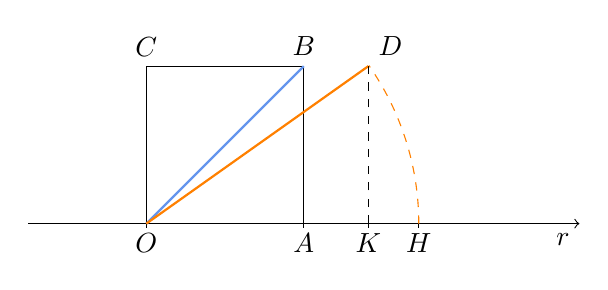
\begin{tikzpicture}[x=10mm, y=10mm]
\draw[->](-3.5,0) -- (3.5,0) node [below left] {$r$};
\foreach \x in {-2,0,.82,1.46}
\draw (\x,1.5pt) -- (\x,-1.5pt);

\foreach \x/\xtext in {-2/O,0/A,0.82/K,1.46/H}
\node[below] at (\x,0) {$\xtext$};

\draw (-2,0) rectangle  (0,2);
\draw[CornflowerBlue,thick] (-2,0) --  (0,2) node[above, black] {$B$};
\draw[orange,thick] (-2,0) --  (0.82,2) node[above right, black] {$D$};
\draw[dashed] (.82,0) -- (.82,2);
   \draw[dashed,orange] (1.46,0) arc [start angle=0, end angle=35,radius=3.5cm];

\node [above] at (-2,2) {$C$};
\end{tikzpicture}
\end{center}
Proseguendo in questo modo possiamo ottenere sulla retta razionale i punti 
associati ai numeri del tipo~${\sqrt{n}}$.

Un'altra classica costruzione, nota come ``spirale di Teodoro'' 
(figura~\ref{fig:D.4}), permette di ottenere i segmenti di misura~$\sqrt{n}$ 
con~$n\in \insN_{0}$.
Si inizia con la costruzione del triangolo rettangolo isoscele di cateto~$1$ 
sappiamo già che la sua ipotenusa è il segmento
di misura~$\sqrt{2}$. Sulla perpendicolare in~$C$ ad~$AC$ si prende il 
segmento~$CD$ di misura~$1$:
applicando il teorema di Pitagora come abbiamo fatto sopra, 
otteniamo~$\overline{AD}=\sqrt{3}$.
Ripetiamo la costruzione dal vertice~$D$ e otteniamo il triangolo 
rettangolo~$ADE$ la cui ipotenusa è~$\overline{AE}=\sqrt{4}$
e poi~$\overline{AF}=\sqrt{5}$ e così via.
\begin{inaccessibleblock}[Figura: TODO]
 \begin{figure}[t]
 \centering% (c) 2012 Dimitrios Vrettos - d.vrettos@gmail.com
\begin{tikzpicture}[x=10mm, y=10mm]
  \tkzDefPoint(0,0){O}
  \tkzDefPoint(2,0){A}
  \tkzDefPoint(2,2){B}

  \tkzDrawPolygon(O,A,B)

  \tkzDrawTriangle[two angles=35.26 and 90](O,B) 
  \tkzGetPoint{C}

  \tkzDrawTriangle[two angles=30 and 90](O,C) 
  \tkzGetPoint{D}

  \tkzDrawTriangle[two angles=26.57 and 90](O,D) 
  \tkzGetPoint{E}

  \tkzDrawTriangle[two angles=24.1 and 90](O,E) 
  \tkzGetPoint{F}

  \tkzDrawTriangle[two angles=22.21 and 90](O,F) 
  \tkzGetPoint{G}

  \tkzLabelPoints[below](O)
  \tkzLabelPoints[right](A,B)
  \tkzLabelPoints[above](C,D,E)
  \tkzLabelPoints[left](F,G)

  \tkzMarkRightAngles[draw=Maroon](O,A,B O,B,C O,C,D O,D,E O,E,F O,F,G)

  \tkzLabelSegment[right](A,B){$1$}
  \tkzLabelSegment[above right](B,C){$1$}
  \tkzLabelSegment[above](C,D){$1$}
  \tkzLabelSegment[above](D,E){$1$}
  \tkzLabelSegment[above left](E,F){$1$}
  \tkzLabelSegment[left](F,G){$1$}

  \tkzLabelSegment[above](O,A){$\sqrt{1}$}
  \tkzLabelSegment[above=4pt](O,B){$\sqrt{2}$}
  \tkzLabelSegment[above left](O,C){$\sqrt{3}$}
  \tkzLabelSegment[above left=6pt](O,D){$\sqrt{4}$}
  \tkzLabelSegment[left=6pt](O,E){$\sqrt{5}$}
  \tkzLabelSegment[below](O,F){$\sqrt{6}$}
  \tkzLabelSegment[below](O,G){$\sqrt{7}$}
\end{tikzpicture}\vspace{-15ex}
 \caption{La spirale di Teodoro.}\label{fig:D.4}
\end{figure}
\end{inaccessibleblock}

% \ovalbox{\risolvii \ref{ese:D.15}, \ref{ese:D.16}, \ref{ese:D.17}}
% 
% \section{Il metodo delle coordinate cartesiane}
% \label{sec:D_coordinate}
% 
% Abbiamo definito prodotto cartesiano di due insiemi non vuoti~$A$ e~$B$ 
% l'insieme formato da tutte
% le coppie ordinate tali che il primo elemento appartenga ad~$A$ e il secondo 
% a~$B$. Mediante proprietà caratteristica
% si scrive:~$A\times B=\{(a;b)/\,a\in A\text{ e }b\in B\}$.
% 
% \begin{exrig}
%  \begin{esempio}
%  \label{ex:D.11}
% Il prodotto cartesiano dei due insiemi~$A=\{1,2,3\}$ e~$B=\{x,y\}$ è
% \[A \times B = \{(1;x), (1;y), (2;x), (2;y), (3;x), (3;y)\}\]
% e graficamente si può rappresentare con un diagramma cartesiano come nella 
% figura~\ref{fig:D.5}.
% 
% Sappiamo che una retta orientata, fissata una unità di misura arbitraria, è 
% l'immagine geometrica dell'insieme dei numeri reali:
% ad ogni numero reale corrisponde un punto della retta e un qualunque punto 
% della retta è immagine di un solo numero reale.
%  \end{esempio}
% \end{exrig}
% 
% \begin{figure}[b]
%  \begin{minipage}[t]{.45\textwidth}
%  \centering% (c) 2012 Dimitrios Vrettos - d.vrettos@gmail.com
\begin{tikzpicture}[x=10mm, y=10mm, smooth]
\begin{scope}[->]
\draw (-.5,0) -- (4,0) node [below]  {$A$};
\draw (0,-.5) -- (0,3)node [left]  {$B$};;
\end{scope}

\foreach \x in {1,2,3}
\draw (\x,1.5pt) -- (\x,-1.5pt);

\foreach \y in {1,2}
\draw (1.5pt,\y) -- (-1.5pt,\y);

\foreach \xi/\xtext in {1/1,2/2,3/3}
\node[below] at (\xi,0) {$\xtext$};

\foreach \yi/\ytext in {1/x,2/y}
\node[left] at (0,\yi){$\ytext$};

\draw[orange, dotted] (0,0) grid (4,3);

\begin{scope}[fill=CornflowerBlue]
\foreach \x in {1,2,3}{
\foreach \y in {1,2}
\filldraw (\x,\y) circle (2pt);
};

\end{scope}
\end{tikzpicture}
%  \caption{Esempio~\ref{ex:D.11}.}\label{fig:D.5}
%  \end{minipage}\hfil
%  \begin{minipage}[t]{.45\textwidth}
%  \centering% (c) 2012 Dimitrios Vrettos - d.vrettos@gmail.com
\begin{tikzpicture}[x=10mm, y=10mm, smooth]
\begin{scope}[->]
\draw (-.5,0) -- (4,0) node [below]  {$x$};
\draw (0,-.5) -- (0,3)node [left]  {$y$};;
\end{scope}

\node[below left] at (0,0) {$O$};

\end{tikzpicture}
%  \caption{Il piano cartesiano.}\label{fig:D.6}
%  \end{minipage}
% 
% \end{figure}
% 
% \subsection{Introduzione al sistema di riferimento cartesiano ortogonale}
% Preso l'insieme~$\insR$ dei numeri reali, costruiamo il prodotto 
% cartesiano~$\insR\times \insR$: esso è costituito dall'insieme delle coppie
% ordinate tali che il primo elemento sia un numero reale come pure il secondo 
% elemento. In~$\insR\times \insR$ avremo coppie il cui primo
% elemento è~$0$, coppie il cui primo elemento è un numero positivo e infine 
% coppie il cui primo elemento è un numero negativo,
% coppie che possiamo sinteticamente rappresentare nel seguente modo:
% \begin{equation*}
% \insR\times \insR=\{(0;0),(0;+),(0;-),(+;0),(-;0),(+;+),(+;-),(-;+),(-;-)\}.
% \end{equation*}
% È possibile dare una rappresentazione grafica di questo insieme di infiniti 
% elementi?
% 
% Consideriamo sul piano una coppia di rette perpendicolari, indichiamo con~$O$ 
% il loro punto di intersezione,
% fissiamo convenzionalmente un verso di percorrenza su ciascuna retta 
% (convenzionalmente sull'orizzontale da
% sinistra a destra, sulla verticale dal basso all'alto) e infine scegliamo un 
% segmento arbitrario come unità di misura.
% Indichiamo con~$x$ l'asse orizzontale che chiamiamo asse delle ascisse e 
% con~$y$ l'asse verticale che chiamiamo asse delle ordinate 
% (figura~\ref{ex:D.6}).
% \begin{definizione}
% Si chiama \emph{riferimento cartesiano ortogonale monometrico} la coppia di 
% rette orientate, perpendicolari, dotate di unità di misura.
% \end{definizione}
% Gli assi dividono il piano in quattro zone chiamate quadranti che sono 
% numerati come in figura~\ref{fig:D.7}.
% Ogni punto dell'asse delle ascisse è immagine di un numero reale:~$O$ è 
% immagine di zero,
% i punti alla sua destra rappresentano i numeri reali positivi, quelli alla sua 
% sinistra tutti i numeri
% reali negativi; analogamente sull'asse delle ordinate il punto~$O$ è immagine 
% dello zero, sopra di questo si collocano i numeri
% positivi e sotto i numeri negativi (figura~\ref{fig:D.8}).
% Per rappresentare gli elementi di~$\insR\times \insR$ cioè le coppie ordinate 
% di numeri reali~$(\alpha; \beta)$ procediamo nel seguente modo:
% \begin{itemize*}
% \item determiniamo sull'asse~$x$ il punto~$A$ immagine del numero 
% reale~$\alpha~$;
% \item da~$A$ tracciamo la retta parallela all'asse~$y$;
% \item determiniamo sull'asse~$y$ il punto~$B$ immagine del numero 
% reale~$\beta~$;
% \item da~$B$ tracciamo la retta parallela all'asse~$x$.
% \end{itemize*}
% Il punto~$P$, intersezione delle parallele tracciate, è l'immagine della 
% coppia ordinata~$(\alpha; \beta)$.
% \begin{figure}[b]
%  \begin{minipage}[t]{.45\textwidth}
%  \centering% (c) 2012 Dimitrios Vrettos - d.vrettos@gmail.com
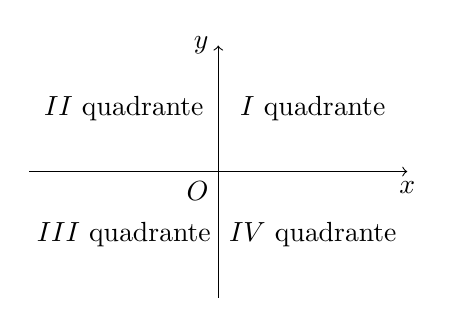
\begin{tikzpicture}[x=8mm, y=8mm, smooth]
\begin{scope}[->]
\draw (0,0) -- (6,0) node [below]  {$x$};
\draw (3,-2) -- (3,2)node [left]  {$y$};;
\end{scope}

\node[below left] at (3,0) {$O$};
\node () at (4.5,1) {$I$ quadrante};
\node () at (1.5,1) {$II$ quadrante};
\node () at (1.5,-1) {$III$ quadrante};
\node () at (4.5,-1) {$IV$ quadrante};
\end{tikzpicture}
%  \caption{I quattro quadranti del piano cartesiano.}\label{fig:D.7}
%  \end{minipage}\hfil
%  \begin{minipage}[t]{.45\textwidth}
%  \centering% (c) 2012 Dimitrios Vrettos - d.vrettos@gmail.com
\begin{tikzpicture}[x=8mm, y=8mm, smooth]
\begin{scope}[->]
\draw (0,0) -- (4,0) node [below]  {$x$};
\draw (2,-2) -- (2,2)node [left]  {$y$};;
\end{scope}

\node[below left] at (2,0) {$O$};
\node[above] at (4,0) {$R^{+}$};
\node[above] at (0,0) {$R^{-}$};
\node[below right] at (2,2) {$R^{+}$};
\node[above right] at (2,-2) {$R^{-}$};
\end{tikzpicture}
%  \caption{Collocazione dei numeri positivi e negativi sul piano 
% cartesiano.}\label{fig:D.8}
%  \end{minipage}
% \end{figure}
% 
% \begin{exrig}
%  \begin{esempio}
%  \label{ex:D.12}
% Determiniamo l'immagine delle coppie ordinate~$(2;3)$ e~$(-1;1)$.
% 
% Nella figura~\ref{fig:D.9} è tracciata la costruzione descritta sopra:~$P$ è 
% il punto del piano immagine della coppia~$(2;3)$ e~$Q$
% è il punto immagine della coppia~$(-1;1)$. Rappresenta le coppie~$(4;-1)$ 
% e~$(-4;1)$.
% Quali punti rappresentano le coppie con un elemento uguale a zero?
%  \end{esempio}
% 
%  \begin{esempio}
%  \label{ex:D.13}
% Determiniamo l'immagine delle seguenti coppie:~$(0;5)$, $(0;-2)$, $(-5;0)$, 
% $(3;0)$.
% 
% Osserviamo (figura~\ref{fig:D.10}) che il punto immagine dello zero 
% sull'asse~$x$ coincide con~$O$, quindi la coppia~$(0;5)$ sarà associata al 
% punto~$R$
% dell'asse~$y$ e la coppia~$(0;-2)$ al punto~$S$ dello stesso asse. 
% Analogamente, poiché il punto immagine dello zero sull'asse~$y$
% coincide con~$O$, le coppie~$(-5;0)$ e~$(3;0)$ sono associate rispettivamente 
% ai punti~$H$ e~$K$ dell'asse~$x$.
%  \end{esempio}
% \end{exrig}
% \begin{figure}[t]
%  \begin{minipage}[t]{.3\textwidth}
%  \centering% (c) 2012 Dimitrios Vrettos - d.vrettos@gmail.com
\begin{tikzpicture}[x=5mm, y=5mm, smooth]
\begin{scope}[->]
\draw (-1.5,0) -- (3.5,0) node [below]  {$x$};
\draw (0,-2.5) -- (0,5.5)node [left]  {$y$};;
\end{scope}

\begin{scope}[dashed, orange]
\draw (-1,0) -- (-1,1);
\draw (-1,1) -- (0,1);
\draw (2,0) -- (2,3);
\draw (2,3) -- (0,3);
\end{scope}

\draw (1,1.5pt) -- (1,-1.5pt) node[below] {1};
\draw (1.5pt,1) -- (-1.5pt,1) node[right] {1};
\node[below left]  at (0,0){$O$};
\filldraw[fill=CornflowerBlue, draw=black] (2,3)circle (1.5pt) node[above] {$P$};
\node[left] at (0,3) {$B$};
\filldraw[fill=CornflowerBlue, draw=black] (-1,1)circle (1.5pt) node[above left] {$Q$};
\node[below] at (2,0) {$A$};
\end{tikzpicture}
%  \caption{Esempio~\ref{ex:D.12}.}\label{fig:D.9}
%  \end{minipage}\hfil
%  \begin{minipage}[t]{.45\textwidth}
%  \centering% (c) 2012 Dimitrios Vrettos - d.vrettos@gmail.com
\begin{tikzpicture}[x=5mm, y=5mm, smooth]
\begin{scope}[->]
\draw (-5.5,0) -- (4.5,0) node [below]  {$x$};
\draw (0,-2.5) -- (0,5.5)node [left]  {$y$};;
\end{scope}

\node[below] at (3,0){3};
\node[below] at (-5,0){$-5$};
\node[left] at (0,5){$5$};
\node[left] at (0,-2){$-2$};

\node[below left]  at (0,0){$O$};
\filldraw[fill=CornflowerBlue, draw=black] (3,0)circle (1.5pt) node[above] {$K$};
\filldraw[fill=CornflowerBlue, draw=black] (0,5)circle (1.5pt) node[right]{$R$};
\filldraw[fill=CornflowerBlue, draw=black] (-5,0)circle (1.5pt) node[above] {$H$};
\filldraw[fill=CornflowerBlue, draw=black] (0,-2)circle (1.5pt) node[right]{$S$};
\end{tikzpicture}
%  \caption{Esempio~\ref{ex:D.13}.}\label{fig:D.10}
%  \end{minipage}\hfil
%  \begin{minipage}[t]{.25\textwidth}
%  \centering% (c) 2012 Dimitrios Vrettos - d.vrettos@gmail.com
\begin{tikzpicture}[x=5mm, y=5mm, smooth]
\begin{scope}[->]
\draw (-1,0) -- (4.5,0) node [below]  {$x$};
\draw (0,-1) -- (0,5.5)node [left]  {$y$};;
\end{scope}

\begin{scope}[orange,dashed]
\draw (0,4) -- (3,4)--(3,0);
\end{scope}
\node[below left]  at (0,0){$O$};
\filldraw[fill=CornflowerBlue, draw=black] (3,0)circle (1.5pt) node[below] {$\alpha$};
\filldraw[fill=CornflowerBlue, draw=black] (3,4)circle (1.5pt) node[right]{$R$};
\filldraw[fill=CornflowerBlue, draw=black] (0,4)circle (1.5pt) node[left]{$\beta$};
\end{tikzpicture}
%  \caption{Ascissa e ordinata di un punto.}\label{fig:D.11}
% \end{minipage}
%  \end{figure}
% 
%  Il punto~$O$ è immagine della coppia~$(0;0)$ ed è chiamato \emph{Origine}.
% \paragraph{Prima conclusione:} ogni coppia di numeri reali è rappresentata da 
% un punto del piano dotato di riferimento cartesiano ortogonale
% monometrico.
% 
% Prendiamo ora un punto~$R$ (figura~\ref{fig:D.11}) del piano sul quale sia 
% stato fissato un riferimento cartesiano ortogonale monometrico e tracciamo 
% da~$R$
% la parallela all'asse~$y$ che interseca l'asse~$x$ nel punto~$A$. A questo 
% punto è associato un numero reale~$\alpha$.
% Analogamente da~$R$ tracciamo la parallela all'asse~$x$ che interseca 
% l'asse~$y$ nel punto~$B$ immagine di un numero reale~$\beta$.
% Al punto~$R$ associamo la coppia di numeri reali~$(\alpha; \beta)$.
% 
% Diremo che~$R$ è il punto di coordinate~$(\alpha;\beta )$, $\alpha~$ si chiama 
% \emph{ascissa} del punto~$R$, $\beta$ \emph{ordinata}
% del punto~$R$.
% 
% \paragraph{Seconda conclusione:} ogni punto del piano dotato di riferimento 
% cartesiano ortogonale monometrico individua una coppia ordinata
% di numeri reali.
% 
% In conclusione, esiste una corrispondenza biunivoca tra l'insieme~$\insR\times 
% \insR$ e l'insieme dei punti del piano dotato di
% riferimento cartesiano ortogonale monometrico. Possiamo dunque ``confondere'' 
% coppia di numeri reali con punto del piano e
% anzi diremo, secondo gli esempi precedenti, ``$P$ è il punto~$(2;3)$, $Q$ il 
% punto~$(-1;1)$'' invece di~``$P$
% è il punto immagine della coppia~$(2;3)$'' o~``$P$ è il punto di 
% coordinate~$(2;3)$''.
% 
% \subsubsection*{Un po' di storia}
% Nel~$II$~secolo~\aC\ Ipparco compilò il primo catalogo stellare in cui precisò 
% la posizione di circa~850 stelle sulla sfera celeste
% mediante due numeri: latitudine e longitudine. La posizione di un punto era 
% dunque individuata attraverso una coppia di numeri.
% Ancora oggi attraverso latitudine e longitudine viene individuato un punto 
% sulla superficie terrestre.
% I romani nel fondare una città segnavano due solchi perpendicolari ai quali 
% riferivano la posizione di case, monumenti, strade.
% 
% Nel~$XVII$~secolo con le opere di Pierre de Fermat e di René Descartes il 
% metodo di rappresentare punti con coppie di numeri divenne
% un procedimento matematico per descrivere enti geometrici attraverso numeri, 
% equazioni, disequazioni e tradurre le relazioni
% tra elementi della geometria in relazioni tra enti dell'algebra.
% 
% La geometria analitica tratta quindi questioni geometriche con metodi di tipo 
% algebrico.
% 
% % \vspazio\ovalbox{\risolvi \ref{ese:D.18}}
% 
% \subsection{Distanza di due punti}
% Assegnato nel riferimento cartesiano ortogonale il punto~$P(\alpha; \beta)$, 
% il numero reale~$|\alpha|$ rappresenta la
% misura della distanza del punto~$P$ dall'asse~$y$ e il numero reale~$|\beta|$ 
% rappresenta la misura della distanza di~$P$
% dall'asse~$x$.
% 
% \begin{figure}[t]
%  \begin{minipage}[t]{.45\textwidth}
%  \centering% (c) 2012 Dimitrios Vrettos - d.vrettos@gmail.com
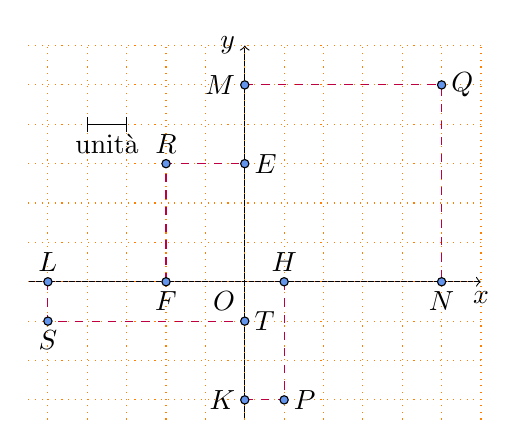
\begin{tikzpicture}[x=5mm, y=5mm, smooth]
  \begin{scope}[->]
    \draw (-5.5,0) -- (6,0) node [below]  {$x$};
    \draw (0,-3.5) -- (0,6)node [left]  {$y$};;
  \end{scope}

  \draw[orange, dotted, step=5mm] (-5.5,-3.5) grid (6,6);
  
  \begin{scope}[purple,dashed]
    \draw (-5,0) -- (-5,-1) --(0,-1);
    \draw (-2,0) -- (-2,3) --(0,3);
    \draw (1,0) -- (1,-3)--(0,-3);
    \draw (0,5) -- (5,5)--(5,0);
  \end{scope}

  \draw[|-|] (-4,4) -- (-3,4) node[below, midway] {unità};

  \node[below left]  at (0,0){$O$};
  
  \begin{scope}[fill=CornflowerBlue, draw=black]
    \filldraw (1,-3)circle (1.5pt) node[right] {$P$};
    \filldraw (5,5)circle (1.5pt) node[right]{$Q$};
    \filldraw (-2,3)circle (1.5pt) node[above] {$R$};
    \filldraw (-5,-1)circle (1.5pt) node[below]{$S$};

    \filldraw (-5,0)circle (1.5pt) node[above]{$L$};
    \filldraw (-2,0)circle (1.5pt) node[below]{$F$};
    \filldraw (0,5)circle (1.5pt) node[left]{$M$};
    \filldraw (0,3)circle (1.5pt) node[right]{$E$};
    \filldraw (0,-1)circle (1.5pt) node[right]{$T$};
    \filldraw (0,-3)circle (1.5pt) node[left]{$K$};
    \filldraw (1,0)circle (1.5pt) node[above]{$H$};
    \filldraw (5,0)circle (1.5pt) node[below]{$N$};
  \end{scope}
\end{tikzpicture}
%  \caption{Esempio~\ref{ex:D.14}.}\label{fig:D.12}
%  \end{minipage}\hfil
%  \begin{minipage}[t]{.45\textwidth}
%  \centering% (c) 2012 Dimitrios Vrettos - d.vrettos@gmail.com
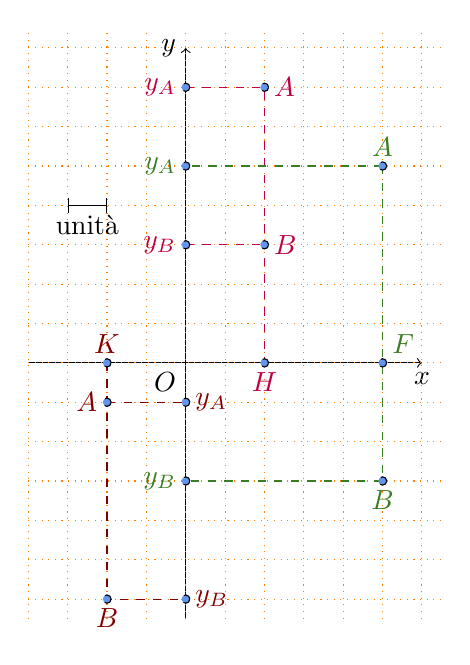
\begin{tikzpicture}[x=5mm, y=5mm, smooth]
  \begin{scope}[->]
    \draw (-4,0) -- (6,0) node [below]  {$x$};
    \draw (0,-6.5) -- (0,8)node [left]  {$y$};;
  \end{scope}

  \draw[dotted,orange, step=5mm] (-4,-6.5) grid (6.5,8.5);

  \draw[|-|] (-3,4) -- (-2,4) node[below, midway] {unità};

  \node[below left]  at (0,0){$O$};
  
  \begin{scope}[every node/.style={purple}, draw=purple, dashed]
    \draw (0,7) -- (2,7)--(2,0);
    \draw (0,3) -- (2,3);
    \begin{scope}[fill=CornflowerBlue, draw=black]
      \filldraw (2,3)circle (1.5pt) node[right, purple] {$B$};
      \filldraw (2,7)circle (1.5pt) node[right]{$A$};
      \filldraw (0,7)circle (1.5pt) node[left]{$y_A$};
      \filldraw (0,3)circle (1.5pt) node[left]{$y_B$};
      \filldraw (2,0)circle (1.5pt) node[below]{$H$};
    \end{scope}
  \end{scope}

  \begin{scope}[every node/.style={OliveGreen},draw=OliveGreen,dashed]
    \draw (5,5) -- (5,-3)--(0,-3);
    \draw (5,5) -- (0,5);
    \begin{scope}[fill=CornflowerBlue, draw=black]
      \filldraw (5,5)circle (1.5pt) node[above] {$A$};
      \filldraw (0,5)circle (1.5pt) node[left]{$y_A$};

      \filldraw (5,-3)circle (1.5pt) node[below]{$B$};
      \filldraw (0,-3)circle (1.5pt) node[left]{$y_B$};

      \filldraw (5,0)circle (1.5pt) node[above right]{$F$};
    \end{scope}
  \end{scope}

  \begin{scope}[every node/.style={Maroon}, draw=Maroon, dashed]
    \draw (-2,0) -- (-2,-6) --(0,-6);
    \draw (-2,-1) -- (0,-1);
    \begin{scope}[fill=CornflowerBlue, draw=black]
      \filldraw (-2,-1)circle (1.5pt) node[left] {$A$};
      \filldraw (0,-1)circle (1.5pt) node[right]{$y_A$};

      \filldraw (-2,-6)circle (1.5pt) node[below]{$B$};
      \filldraw (0,-6)circle (1.5pt) node[right]{$y_B$};

      \filldraw (-2,0)circle (1.5pt) node[above]{$K$};
    \end{scope}
  \end{scope}
\end{tikzpicture}
%  \caption{Esempio~\ref{ex:D.16}.}\label{fig:D.13}
%  \end{minipage}
%  \end{figure}
% 
% \begin{exrig}
%  \begin{esempio}
%  \label{ex:D.14}
% Determinare la misura della distanza dagli assi coordinati dei 
% punti~$P(+1;-3)$, $Q(+5;+5)$, $R(-2;+3)$, $S(-5;-1)$ (figura~\ref{fig:D.12}).
% 
% \emph{Dati}:~$P(+1;-3)$.
% 
% \emph{Obiettivo}:~$PH\perp$ asse~$x$, il segmento~$PH$ è la distanza di~$P$ 
% dall'asse~$x$;
% $PK\perp$ asse~$y$, il segmento~$PK$ è la distanza di~$P$ dall'asse~$y$.
% 
% Per quanto detto sopra si ha~$\overline{PH}=|-3|=-(-3)=3$; 
% $\overline{PH}=|+1|=1$.
% Completate la soluzione dell'esempio, seguendo la traccia.
%  \end{esempio}
% \end{exrig}
% 
% Vogliamo ora determinare la misura~$\overline{AB}$ di un segmento~$AB$, 
% inserito in un riferimento cartesiano ortogonale
% monometrico~$O_{xy}$, conoscendo le coordinate degli estremi~$A$ e~$B$ del 
% segmento stesso.
% 
% \begin{figure}[t]
%  \begin{minipage}[t]{.45\textwidth}
%  \centering% (c) 2012 Dimitrios Vrettos - d.vrettos@gmail.com
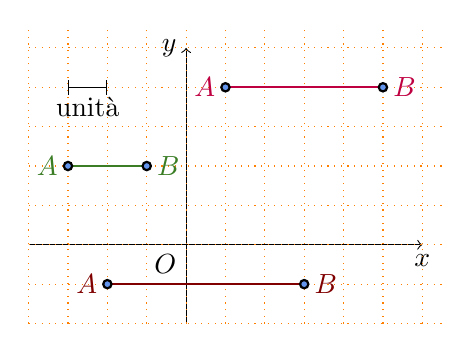
\begin{tikzpicture}[x=5mm, y=5mm, smooth]
  \begin{scope}[->]
    \draw (-4,0) -- (6,0) node [below]  {$x$};
    \draw (0,-2) -- (0,5)node [left]  {$y$};;
  \end{scope}

  \draw[dotted,orange, step=5mm] (-4,-2) grid (6.5,5.5);

  \draw[|-|] (-3,4) -- (-2,4) node[below, midway] {unità};

  \node[below left]  at (0,0){$O$};
  
  \begin{scope}[every node/.style={purple}, draw=purple,thick]
    \draw (1,4) -- (5,4);
    \begin{scope}[fill=CornflowerBlue, draw=black]
      \filldraw (5,4)circle (1.5pt) node[right, purple] {$B$};
      \filldraw (1,4)circle (1.5pt) node[left]{$A$};
    \end{scope}
  \end{scope}

  \begin{scope}[every node/.style={OliveGreen},draw=OliveGreen,thick]
    \draw (-3,2) -- (-1,2);
    \begin{scope}[fill=CornflowerBlue, draw=black]
      \filldraw (-3,2)circle (1.5pt) node[left] {$A$};
      \filldraw (-1,2)circle (1.5pt) node[right]{$B$};
    \end{scope}
  \end{scope}

  \begin{scope}[every node/.style={Maroon}, draw=Maroon, thick]
    \draw (-2,-1) -- (3,-1);
    \begin{scope}[fill=CornflowerBlue, draw=black]
      \filldraw (-2,-1)circle (1.5pt) node[left] {$A$};
      \filldraw (3,-1)circle (1.5pt) node[right]{$B$};
    \end{scope}
  \end{scope}
\end{tikzpicture}
%  \caption{I due punti hanno la stessa ordinata.}\label{fig:D.14}
%  \end{minipage}\hfil
%  \begin{minipage}[t]{.45\textwidth}
%  \centering% (c) 2012 Dimitrios Vrettos - d.vrettos@gmail.com
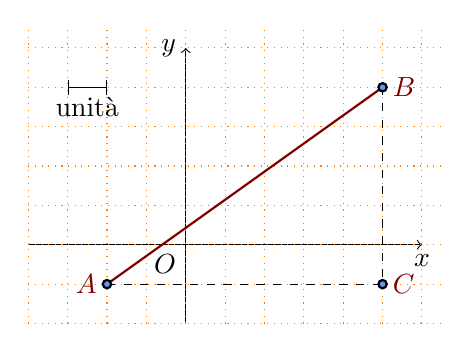
\begin{tikzpicture}[x=5mm, y=5mm, smooth]
  \begin{scope}[->]
    \draw (-4,0) -- (6,0) node [below]  {$x$};
    \draw (0,-2) -- (0,5)node [left]  {$y$};;
  \end{scope}

  \draw[dotted,orange, step=5mm] (-4,-2) grid (6.5,5.5);

  \draw[|-|] (-3,4) -- (-2,4) node[below, midway] {unità};

  \node[below left]  at (0,0){$O$};
  	\draw[dashed,thin] (-2,-1) -- (5,-1)--(5,4);
  \begin{scope}[every node/.style={Maroon}, draw=Maroon, thick]
    \draw (-2,-1) -- (5,4);
    \begin{scope}[fill=CornflowerBlue, draw=black]
      \filldraw (-2,-1)circle (1.5pt) node[left] {$A$};
      \filldraw (5,4)circle (1.5pt) node[right]{$B$};
      \filldraw (5,-1)circle (1.5pt) node[right]{$C$};

    \end{scope}
  \end{scope}
\end{tikzpicture}
%  \caption{Il segmento ha una direzione diversa da quella degli assi 
% coordinati.}\label{fig:D.15}
%  \end{minipage}
%  \end{figure}
% \paragraph{Caso I} i due punti hanno la stessa ascissa. Il segmento~$AB$ è 
% parallelo all'asse~$y$ e può
% presentarsi in diverse posizioni rispetto all'asse~$x$.
% \begin{exrig}
%  \begin{esempio}
% Determinare la misura della distanza dei punti~$A(2;7)$ e~$B(2;3)$.
% 
% \emph{Dati}:~$A(2;7)$, $B(2;3)$.
% 
% \emph{Obiettivo}:~$\overline{AB}$.
% 
% \emph{Procedura 
% risolutiva}:~$\overline{AB}=\overline{AH}-\overline{BH}=y_{A}-y_{B}=7-3=4$.
% 
%  \end{esempio}
%  \begin{esempio}
%  \label{ex:D.16}
% Determinare la misura della distanza dei punti~$A(5;5)$ e~$B(5;-3)$ 
% (figura~\ref{fig:D.13}).
% 
% \emph{Dati}:~$A(5;5)$, $B(5;-3)$.
% 
% \emph{Obiettivo}:~$\overline{AB}$.
% 
% \emph{Procedura 
% risolutiva}:~$\overline{AB}=\overline{AF}+\overline{BF}=y_{A}+(-y_{B})=y_{A}-y_{
% B}=5-(-3)=8$.
% 
%  \end{esempio}
%  \begin{esempio}
% Determinare la misura della distanza dei punti~$A(-2;-1)$ e~$B(-2;-6)$.
% 
% \emph{Dati}:~$A(-2;-1)$, $B(-2;-6)$.
% 
% \emph{Obiettivo}:~$\overline{AB}$.
% 
% \emph{Procedura 
% risolutiva}:~$\overline{AB}=\overline{BK}-\overline{AK}=-(y_{B})-(-y_{A})=y_{A}
% -y_{B}=-1+6=5$.
% 
%  \end{esempio}
% \end{exrig}
% Osserviamo che in ogni caso abbiamo sottratto dall'ordinata maggiore 
% l'ordinata minore; generalizzando possiamo concludere:
% la \emph{misura del segmento} $AB$ \emph{parallelo all'asse delle ordinate} 
% è~$\overline{AB}=|x_{a}-x_{B}|$
% indipendentemente da quale estremo abbia ordinata maggiore.
% 
% \paragraph{Caso II} i due punti hanno la stessa ordinata. Il segmento~$AB$ 
% (figura~\ref{fig:D.14}) è parallelo all'asse~$x$ e
% può presentarsi in diverse posizioni rispetto all'asse~$y$.
% 
% Seguendo il procedimento applicato nel primo caso, dopo aver rilevato le 
% coordinate degli estremi del segmento~$AB$
% nella figura accanto, verifica che in ogni caso~$\overline{AB}=|x_{A}-x_{B}|$.
% 
% La \emph{misura del segmento} $AB$ \emph{parallelo all'asse delle ascisse} 
% è~$\overline{AB}=|x_{A}-x_{B}|$
% indipendentemente da quale estremo abbia ascissa maggiore.
% 
% \paragraph{Caso III} è questo il caso generale: il segmento ha una direzione 
% diversa da quella degli assi coordinati (figura~\ref{fig:D.15}).
% 
% \emph{Dati}:~$A(x_A;x_B)$, $B(y_A;y_B)$.
% 
% \emph{Obiettivo}:~$\overline{AB}$.
% 
% \emph{Procedura risolutiva}: tracciando da~$A$ la parallela all'asse~$x$ e 
% da~$B$ la parallela all'asse~$y$
% si determina il vertice~$C$ del triangolo rettangolo~$ABC$ di cui~$AB$ è 
% l'ipotenusa.
% Per il teorema di Pitagora si ottiene:~$\overline{AB}=\sqrt{\overline{AC}^2 + 
% \overline{BC}^2}=\sqrt{\left(x_A-x_C \right)^2+
% \left(y_C-y_B \right)^2}$. %----figura18
% Poiché $x_{C}=x_{B}$ e~$y_{C}=y_{A}$ sostituendo si ha:
% 
% $\overline{AB}=\sqrt{\left(x_{A}-x_{B}\right)^{2}+\left(y_{A}-y_{B}\right)^{2}}
% $.
% 
% La \emph{misura del segmento} $AB$, \emph{note le coordinate} dei suoi estremi 
% è:
% 
% \[\overline{AB}=\sqrt{\left(x_{A}-x_{B}\right)^{2}+\left(y_{A}-y_{B}\right)^{2}}
% .\]
% 
% % \ovalbox{\risolvii \ref{ese:D.19}, \ref{ese:D.20}, \ref{ese:D.21}, 
% \ref{ese:D.22}, \ref{ese:D.23}, \ref{ese:D.24}, \ref{ese:D.25}, \ref{ese:D.26},
% % \ref{ese:D.27}, \ref{ese:D.28}, \ref{ese:D.29}, \ref{ese:D.30}}
% 
% % \vspazio\ovalbox{\ref{ese:D.31}}
% \subsection{Punto medio di un segmento}
% Ricordiamo il teorema di Talete:
% 
% \begin{teorema}[di Talete]
% In un fascio di rette parallele tagliato da due trasversali, a segmenti 
% congruenti
% su una trasversale corrispondono segmenti congruenti sull'altra trasversale.
% Cioè, se~$AB=BC$ allora~$A'B'=B'C'$.
% \end{teorema}
% 
% \begin{figure}[h]
%  \centering% (c) 2012 Dimitrios Vrettos - d.vrettos@gmail.com
\begin{tikzpicture}[x=10mm, y=10mm, smooth]
\tkzSetUpPoint[shape=circle,size=7pt,color=black, fill=CornflowerBlue]
\tkzDefPoints{0/0/a1, 4/0/a2, 0/-1/b1, 4/-1/b2, 0/-2/c1, 4/-2/c2}

\tkzSetUpLine[color=Maroon]
\tkzDrawLine[end= $a$](a1,a2)
\tkzDrawLine[end= $b$](b1,b2)
\tkzDrawLine[end= $c$](c1,c2) 

\tkzDefPoints{1/0/A, 2.8/0/A', 0/-2/C, 4/-2/C'}

\tkzDefLine(C,A)
\tkzInterLL(C,A)(b1,b2) \tkzGetPoint{B}

\tkzDefLine(C',A')
\tkzInterLL(C',A')(b1,b2) \tkzGetPoint{B'}

\tkzSetUpLine[color=OliveGreen]
\tkzDrawLine[end= $r$](C,A)
\tkzDrawLine[end= $r'$](C',A')

\tkzDrawPoints(A,A',B,B',C,C')
\tkzLabelPoints[above left](A,B,C)
\tkzLabelPoints[above right](A',B',C')
\end{tikzpicture}
%  \caption{Il teorema di Talete.}\label{fig:D.16}
%  \end{figure}
% 
% 
% 
% Richiamiamo anche la definizione di punto medio di un segmento:
% \begin{definizione}
%  Il punto medio di un segmento~$AB$ è il punto interno
% al segmento che lo divide in due parti congruenti:~$AM\equiv MB$.
% \end{definizione}
% 
%   \begin{figure}[h]
%   \centering% (c) 2012 Dimitrios Vrettos - d.vrettos@gmail.com
\begin{tikzpicture}[x=10mm, y=10mm, smooth]
	\tkzSetUpPoint[shape=circle,size=7pt,color=black, fill=CornflowerBlue]

	\tkzDefPoint(0,2){A}
	\tkzDefPoint(4,2){B}
	\tkzDefMidPoint(A,B) 
	\tkzGetPoint{M}
	
	\tkzDrawSegment[style={thick, Maroon}](A,B)    
	\tkzLabelPoints[above](A,B,M)

	\tkzDrawPoints(A,B,M)

\end{tikzpicture}
%   \caption{Il punto medio.}\label{fig:D.17}
%  \end{figure}
% 
% \newpage
% %\begin{problema}
% \begin{exrig}
%  \begin{esempio}
% \label{ex:D.18}
%  Conoscendo le coordinate degli estremi~$A$ e~$B$ di un segmento determiniamo
% le coordinate del suo punto medio (figura~\ref{fig:D.18}).
% %\end{problema}
% 
% %\begin{soluzione}
% \emph{Dati}:~$A(x_A;x_B)$, $B(y_A;y_B)$, $AM \equiv MB$.
% 
% \emph{Obiettivo}:~$M(x_{M};y_{M})$.
% 
% \emph{Procedura risolutiva}: essendo~$AM\equiv MB$ per il teorema di 
% Talete~$A'M'\equiv M'B'$;
% si ha inoltre~$A'(x_{A};0)$, $B'(x_{B};0)$, $M'(x_{M};0)$ e 
% quindi~$x_{M}-x_{A}=x_{B}-x_{M}$
% da cui~$2x_{M}=x_{A}+x_{B}$ e dunque~$x_{M}=\dfrac{x_{A}+x_{B}}{2}$.
% Con ragionamento analogo tracciando dai punti~$A$, $B$, $M$ le parallele 
% all'asse~$x$ si ricava~$y_{M}=\dfrac{y_{A}+y_{B}}{2}$.
% 
% Le \emph{coordinate del punto medio} $M$ di un segmento~$AB$, 
% con~$A(x_{A};x_{B}),B(x_{B};y_{B})$ sono:
% \[x_{M}=\dfrac{x_{A}+x_{B}}{2};\, y_{M}=\dfrac{y_{A}+y_{B}}{2}.\]
% %\end{soluzione}
% \end{esempio}
% 
% \begin{figure}[t]
%    \centering% (c) 2012 Dimitrios Vrettos - d.vrettos@gmail.com
\begin{tikzpicture}[x=10mm, y=10mm, smooth]
  \tikzset{xaxe style/.style ={->}}

  \tkzInit[xmin=-.5,xmax=5,ymin=-.5,ymax=4]

  \clip (-.5,-.5) rectangle (6,5);

  \tkzDrawX[noticks,below]
  \tkzDrawY[noticks] 

  \tkzSetUpPoint[shape=circle,size=7pt,color=black, fill=CornflowerBlue]

  \tkzDefPoint(0,0){o}
  \tkzDefPoint(6,0){x}

  \tkzDefPoint(0,0){O}
  \tkzDefPoint(1,4){A}
  \tkzDefPoint(5,2){B}
  \tkzDefMidPoint(A,B) 
  \tkzGetPoint{M}

  \tkzDrawSegment[style={thick, Maroon}](A,B)    
  \tkzLabelPoints[above](A,B,M)

  \tkzDefPointBy[projection=onto o--x](A) \tkzGetPoint{A'}
  \tkzDefPointBy[projection=onto o--x](B) \tkzGetPoint{B'}
  \tkzDefPointBy[projection=onto o--x](M) \tkzGetPoint{M'}

  \tkzLabelPoints[below](A',B',M')
  \tkzLabelPoints[below left](O)

  \tkzDrawSegment[style=dashed](A,A')
  \tkzDrawSegment[style=dashed](B,B')

  \tkzDrawSegment[style=dotted](M,M')

  \tkzDrawPoints(A,B,M)
  \tkzDrawPoints(A',B',M')
\end{tikzpicture}
%   \caption{Esempio~\ref{ex:D.18}.}\label{fig:D.18}
% \end{figure}
% 
% %\begin{exrig}
%  \begin{esempio}
% Determinare le coordinate del punto medio del segmento di 
% estremi~$A\left(-{\frac{3}{4}};1\right)$, $B\left(2;-\frac{1}{2}\right)$.
% 
% \emph{Dati}:~$A\left(-{\frac{3}{4}};1\right)$, $B\left(2;-\frac{1}{2}\right)$, 
% $AM \equiv MB$.
% 
% \emph{Obiettivo}:~$M(x_{M};y_{M})$.
% 
% \emph{Procedura 
% risolutiva}:~$x_{M}=\frac{x_{A}+x_{B}}{2}=\frac{-{\frac{3}{4}}+2}{2}=\frac{5}{8}
% $;\,
% $y_{M}=\frac{1+\left(-{\frac{1}{2}}\right)}{2}=\frac{1}{4}$ 
% quindi~$M\left(\frac{5}{8};\frac{1}{4}\right)$.
%  \end{esempio}
% \end{exrig}
% 
% % \ovalbox{\risolvii \ref{ese:D.32}, \ref{ese:D.33}, \ref{ese:D.34}, 
% \ref{ese:D.35}, \ref{ese:D.36}}

% \newpage

\end{comment}

\subsection{Il grafico di una funzione}
\label{subsec:fun_grafico}

Ricordiamo le seguente definizione.
\begin{definizione}
 Una funzione~$f$ è una corrispondenza univoca tra due insiemi non vuoti: ad 
ogni elemento~$x$ (variabile indipendente)
del dominio associa uno e un solo valore~$y$ della variabile dipendente.

 L'elemento~$y$, corrispondente di un elemento~$x$ del dominio, viene detto 
\emph{immagine di}~$x$ nella funzione~$f$ e si scrive~$y=f(x)$ che si legge 
\emph{y uguale effe di x}.
\end{definizione}
Le funzioni numeriche, cioè aventi per dominio e codominio insiemi numerici, 
possono essere espresse:
\begin{itemize*}
\item con \emph{linguaggio comune}, purché in modo preciso e inequivocabile: 
esempio: La funzione~$f$
 ``associa ad ogni numero razionale il suo triplo'';
\item attraverso un \emph{algoritmo} (figura~\ref{fig:D.19}), cioè una serie di 
istruzioni per trasformare il valore della variabile indipendente
 (in ingresso) nel valore della variabile dipendente (in uscita);
\item mediante una \emph{tabella}:
 \begin{center}
\begin{tabular}{cccccc}
 \toprule
 $x$ & $-2$ & $0$ & $3$ & $7$ & $10$ \\
 $y$ & $-6$ & $0$ & $9$ & $21$ & $30$\\
 \bottomrule
 \end{tabular}
 \end{center}
\item con una \emph{formula} che indica il calcolo che si effettua sulla 
variabile indipendente per determinare in modo univoco
il valore della variabile dipendente. Per esempio:~$y=3x$.
\end{itemize*}

\begin{inaccessibleblock}[Figura: TODO]
 \begin{figure}[b]
\centering% (c) 2012 Dimitrios Vrettos - d.vrettos@gmail.com
\begin{tikzpicture} [auto,block/.style={rectangle, draw=Maroon, thick, text width=5.3em,align=center, rounded corners, minimum height=4em},%
block1/.style={rectangle, draw=Maroon, thick, text width=8em,align=center, rounded corners, minimum height=4em},%
cloud/.style={draw=CornflowerBlue, thick, ellipse, minimum height=2.2em},%
line/.style ={draw, thick, ->,shorten >=2pt}]

  \matrix [column sep=7mm]{
    \node [block] (prn) {prendi un numero razionale}; 
    & \node [block] (molt) {moltiplicalo per 3}; 
    & \node [block] (scr) {scrivi il risultato}; \\
  };
  
  \begin{scope}[every path/.style=line]
    \path (prn)-- (molt);
    \path (molt) -- (scr);
  \end{scope}

  \begin{scope}[yshift=-30mm]
    \matrix [column sep=14mm, row sep=7mm]{
      \node [block1] (ind) {Variabile indipendente: $x$}; 
      & \node [block1] (dip) {Variabile dipendente: $y$}; \\
      \node[cloud] (ing) {Valore in ingresso};
      &\node[cloud] (usc) {Valore in uscita};\\
    };

    \begin{scope}[every path/.style=line]
      \path (ind)--  node [midway]{$f$} (dip);
      \path (ing) --(ind);
      \path(dip)--(usc);
    \end{scope}
  \end{scope}
\end{tikzpicture}
  
\caption{Funzione numerica espressa tramite un algoritmo.}\label{fig:D.19}
\end{figure}
\end{inaccessibleblock}

\begin{exrig}
 \begin{esempio}
Traccia su un piano quadrettato un riferimento cartesiano ortogonale 
monometrico.
Completa la tabella per la funzione~$y=2x$ avente come dominio e codominio 
l'insieme~$\insR$ dei numeri reali.
\begin{center}
 \begin{tabular}{ccccccc}
 \toprule
 $x$ & $0$ && $1/2$ & $2$ & $-3$ &\\
 $y$ &&$2$&&&&$5$\\
 \bottomrule
 \end{tabular}
\end{center}
Ogni coppia~$(x;y)$ determina nel riferimento cartesiano un punto; rappresenta i 
punti le cui coordinate sono
le coppie ordinate contenute nella tabella. Puoi osservare che i punti trovati 
sono allineati su una retta passante
per l'origine del riferimento.
 \end{esempio}
\end{exrig}
\begin{definizione}
 Si chiama \emph{grafico di una funzione} l'insieme di tutti e soli i punti del 
piano cartesiano che
 rappresentano le coppie ordinate costruite tramite la funzione assegnata.
\end{definizione}
\osservazione
I pochi punti ottenuti dalla compilazione della tabella possono essere uniti con 
un tratto continuo perché
assegnando alla variabile indipendente altri valori reali, ad esempio compresi 
tra~$0$ e~$2$, si potrebbero
determinare infiniti punti che risulterebbero allineati con i precedenti.

% \vspazio\ovalbox{\risolvii \ref{ese:D.37}, \ref{ese:D.38}}

\subsection{Proporzionalità diretta e inversa}
\label{subsec:fun_proporzionalita}

\subsubsection{La funzione di proporzionalità diretta}

\begin{center}
 \begin{tabular}{ccccccc}
 \toprule
 $x$ & $0$ & $-1$ & $ 1/2$ & $2$ & $-3$ & $-5/2$\\
 $y$ & $0$ & $2$ & $-1$ & $-4$ & $6$ & $5$\\
 \midrule
 y/x& & & & & & \\
 \bottomrule
 \end{tabular}
\end{center}
Compila la terza riga della tabella contenente il rapporto tra la variabile 
dipendente~$y$ e la variabile indipendente~$x$.
Cosa osservi? Completa:~$\dfrac{y}{x}=\dotfill$
\begin{definizione}
 Una funzione in cui risulta \emph{costante e diverso da zero il rapporto} tra 
la variabile dipendente e la variabile indipendente
 si chiama \emph{funzione di proporzionalità diretta}. In simboli, $y$ 
direttamente proporzionale a
$x \Leftrightarrow \dfrac{y}{x}=k$ con~$k\in \insR$ e~$k\neq~0$ o 
anche~$y=k\cdot x$.
\end{definizione}
Il grafico di una funzione di proporzionalità diretta è una \emph{retta passante 
per l'origine};
la costante~$k$ si chiama \emph{coefficiente angolare} della retta.

Nella figura~\ref{fig:D.20} è rappresentata una retta passante per l'origine del 
riferimento; essa forma con l'asse orientato delle
$x$ un angolo~$\alpha~$ la costante~$k$ ci dà informazioni su tale angolo.
In particolare se la costante di proporzionalità è \emph{positiva}, 
l'angolo~$\alpha$ è \emph{acuto}, se la costante è
\emph{negativa} allora l'angolo~$\alpha$ è \emph{ottuso}. Se $k=1$ l'angolo è 
di~45° e la retta è la bisettrice.

\begin{inaccessibleblock}[Figura: TODO]
 \begin{figure}[h]
 \begin{minipage}[t]{.45\textwidth}
  \centering% (c) 2012 Dimitrios Vrettos - d.vrettos@gmail.com
\begin{tikzpicture}[x=10mm, y=10mm, smooth]
  \tikzset{xaxe style/.style ={->}}
  \tkzInit[xmin=-.5,xmax=3,ymin=-.5,ymax=3]

  \clip (-.5,-.5) rectangle (4,4);

  \tkzDefPoint(0,0){o}
  \tkzDefPoint(6,0){x}

  \tkzDefPoint(0,0){O}
  \tkzDefPoint(1,0){A}
  \tkzDefPoint(2,2){B}

  \tkzMarkAngle[arc=l,size=1 cm,fill=LimeGreen](A,O,B)
  \tkzLabelAngle[pos=1.3](A,O,B){$\alpha$}

  \tkzDrawX[noticks,below]
  \tkzDrawY[noticks] 

  \tkzLabelPoints[above left](O)

  \draw[Maroon, thick] (-.5,-.5)--(3,3);
\end{tikzpicture}
  \caption{Coefficiente angolare di una funzione.}\label{fig:D.20}
 \end{minipage}\hfil
 \begin{minipage}[t]{.45\textwidth}
  \centering% (c) 2012 Dimitrios Vrettos - d.vrettos@gmail.com
\begin{tikzpicture}[x=10mm, y=10mm]

\clip (-.5,-.5) rectangle (4,4);

\tkzDefPoint(0,0){A}
\tkzDefPoint(3,0){B}
\tkzDefPoint(3,3){C}
\tkzDefPoint(0,3){D}

\tkzDrawSegment(A,B)
\tkzDrawSegment(C,B)
\tkzDrawSegment(C,D)
\tkzDrawSegment(A,D)

 \tkzLabelPoints[below left](A)
 \tkzLabelPoints[below right](B)
 \tkzLabelPoints[above right](C)
 \tkzLabelPoints[above left](D)

\draw[CornflowerBlue, thick] (0,0)--(3,3);
\end{tikzpicture}
  \caption{Il quadrato~$ABCD$ del problema~\ref{ex:D.21}.}\label{fig:D.21}
 \end{minipage}
\end{figure}
\end{inaccessibleblock}

\begin{problema}
\label{ex:D.21}
Nel quadrato~$ABCD$ (figura~\ref{fig:D.21}) il cui lato misura~$x$, determinare 
il perimetro e la diagonale.
\end{problema}
\begin{soluzione}
 Abbiamo i dati:~$\overline{AB}=x$ con~$x>0$ e l'obiettivo:~$2p$, 
$\overline{AC}$.

 $2p=4\cdot x$, al variare del lato varia il perimetro, che risulta essere 
dunque funzione del lato.
Indicato con~$y$ il perimetro scriviamo~$y=4x$, funzione di proporzionalità 
diretta con~$\Dom=\insR^{+}$,
coefficiente~$k=4$. La rappresentazione grafica di questa funzione è una 
semiretta contenuta nel primo quadrante,
ma privata del suo punto origine (figura~\ref{fig:D.22}).

Determiniamo ora la diagonale: per il teorema di Pitagora si ha
\begin{align*}
 &\overline{AC}^{2}=\overline{AB}^{2}+\overline{BC}^{2}=x^{2}+x^{2}=2x^{2}\\
 &\overline{AC}=\sqrt{2\cdot x^{2}}=x\cdot \sqrt{2}.
\end{align*}

Indicando con~$y$ la diagonale si ha la funzione di proporzionalità 
diretta~$y=\sqrt{2}\cdot x$
con coefficiente~$k=\sqrt{2}$, di dominio~$\Dom=\insR^{+}$.
La rappresentazione grafica di questa funzione è una semiretta contenuta nel 
primo quadrante, ma privata del suo punto origine (figura~\ref{fig:D.23}).
\end{soluzione}

\begin{inaccessibleblock}[Figura: TODO]
 \begin{figure}[h]
 \begin{minipage}[b]{.45\textwidth}
  \centering% (c) 2012 Dimitrios Vrettos - d.vrettos@gmail.com
\begin{tikzpicture}[x=7mm, y=7mm, smooth]
\begin{scope}[dotted,orange]
\draw[step=7mm] (-1.5,-1) grid (5.5,6);
\end{scope}
\begin{scope}[->]
\draw (-.5,0) -- (5,0) node [below]  {lato};
\draw (0,-.5) -- (0,5.5) node [left]   {$2p$};
\end{scope}
\foreach \x/\xtext in {1/1,2/2,4/4}
\draw (\x,1.5pt) -- (\x,-1.5pt) node[below] {\xtext};
\foreach \y/\ytext in {1/2,2/4,4/8}
\draw (1.5pt,\y) -- (-1.5pt,\y) node[left] {$\ytext$};

\begin{scope}[dashed]
\draw (1,0) -- (1,1) --(0,1);
\draw (2,0) -- (2,2) --(0,2);
\draw (4,0) -- (4,4) --(0,4);
\end{scope}
\draw[Maroon, thick] (0,0)--(4,4);


\node[below left] at (0,0) {0};
\filldraw[fill=white, draw=black] (0,0) circle (2pt);

\end{tikzpicture}
  \caption{Il perimetro~$2p$ in funzione del lato.}\label{fig:D.22}
 \end{minipage}\hfil
 \begin{minipage}[b]{.45\textwidth}
  \centering% (c) 2012 Dimitrios Vrettos - d.vrettos@gmail.com
\begin{tikzpicture}[x=7mm, y=7mm, smooth]
\begin{scope}[dotted,orange]
\draw[step=7mm] (-1.5,-1) grid (5.5,7);
\end{scope}
\begin{scope}[->]
\draw (-.5,0) -- (5,0) node [below]  {lato};
\draw (0,-.5) -- (0,6.5) node [above]   {diagonale};
\end{scope}
\foreach \x/\xtext in {1/1,2/2,4/4}
\draw (\x,1.5pt) -- (\x,-1.5pt) node[below] {\xtext};
\foreach \y/\ytext in {1.414/\sqrt{2},2.828/2\sqrt{2},5.687/4\sqrt{2}}
\draw (1.5pt,\y) -- (-1.5pt,\y) node[left] {$\ytext$};

\begin{scope}[dashed]
\draw (1,0) -- (1,1.414) --(0,1.414);
\draw (2,0) -- (2,2.828) --(0,2.828);
\draw (4,0) -- (4,5.687) --(0,5.687);
\end{scope}
\draw[Maroon, thick] (0,0)--(4,5.687);


\node[below left] at (0,0) {0};
\filldraw[fill=white, draw=black] (0,0) circle (2pt);

\end{tikzpicture}
  \caption{La diagonale in funzione del lato.}\label{fig:D.23}
 \end{minipage}
\end{figure}
\end{inaccessibleblock}

% \vspazio\ovalbox{\risolvii \ref{ese:D.39}, \ref{ese:D.40}, \ref{ese:D.41}, 
% \ref{ese:D.42}, \ref{ese:D.43}}

\subsubsection{La funzione di proporzionalità inversa}
\begin{problema}
La base e l'altezza di un rettangolo~$ABCD$ misurano 
rispettivamente~$3\unit{cm}$ e~$4\unit{cm}$.
Determina la sua area.
\begin{soluzione}
 \dotfill
\end{soluzione}

Se le misure dei lati sono numeri interi, esistono altri rettangoli equivalenti 
a quello dato?
Costruisci i rettangoli equivalenti, indicando accanto a ciascuno la misura dei 
lati.
Se le misure fossero numeri reali, potresti determinare \emph{tutti} i 
rettangoli equivalenti a quello assegnato?

\emph{Generalizziamo}: i lati~$x$ e~$y$ di tutti i rettangoli equivalenti a 
quello dato sono legati dalla condizione~$x\cdot y=12$ con~$x\in \insR^{+}$ 
e~$y\in \insR^{+}$.
\begin{center}
 \begin{tabular}{cccccc}
 \toprule
 $x$ & $6$ & $8$ & $10$ & $1/3$ & $4/3$\\
 $y$ & $2$ & $3/2$ & $6/5$ & $36$ & $9$\\
 \bottomrule
 \end{tabular}
\end{center}
Osserviamo che se fissiamo il valore di~$x$ il lato~$y$ vale~$y=\frac{12}{x}$ 
come nella tabella.
Rappresenta ora nel riferimento cartesiano ortogonale i punti individuati dalla 
tabella: essi si collocano
nel primo quadrante perché $\ldots \ldots \ldots$ Ti sembrano allineati?
\end{problema}
\begin{definizione}
Una funzione in cui \emph{il prodotto} tra la variabile dipendente e la 
variabile indipendente risulta \emph{costante e diverso da zero}
si chiama \emph{funzione di proporzionalità inversa}. In simboli:~$y$ 
inversamente proporzionale a~$x \Leftrightarrow x\cdot y=k$
con~$k\in \insR_{0}$ e~$x\neq~0$ o anche~$y=\dfrac{k}{x}$.
\end{definizione}

Il grafico di una funzione di \emph{proporzionalità inversa} è una curva 
chiamata \emph{iperbole}.

Analizziamo tale funzione e rappresentiamo il suo grafico a secondo dei valori 
della costante~$k$.

\paragraph{Caso~$k>0$} Quando ci proponiamo di costruire una tabella di valori, 
le variabili~$x$ e~$y$ sono
senz'altro concordi; al numero positivo~$x$ corrisponde il numero 
positivo~$y=\frac{k}{x}$ dunque i punti
nel riferimento cartesiano si collocano nel primo quadrante; al numero 
negativo~$x$ corrisponde il numero
negativo~$y=\frac{k}{x}$ dunque i punti nel riferimento cartesiano si collocano 
nel terzo quadrante.
\begin{exrig}
 \begin{esempio}
Rappresentare graficamente la funzione~$y=\frac{2}{x}$.
Per far questo assegniamo a~$x$ alcuni valori, positivi e negativi:
\begin{center}
 \begin{tabular}{cccccccc}
 \toprule
 $x$ & $-3$ & $-1$ & $-1/2$ & $1$ & $4$& $1/2$ & $3$\\
 $y$ & $-2/3$ & $-2$ & $-4$ & $2$ & $1/2$& $4$ & $2/3$\\
 \bottomrule
 \end{tabular}
\end{center}
Riportiamo i punti nel riferimento cartesiano ortogonale. Essi si collocano nel 
primo e terzo quadrante come previsto,
non sono allineati. Non possiamo attribuire alla variabile indipendente il 
valore zero perché non si può dividere per zero,
né alcun valore di~$x$ potrà avere come immagine~$y=0$ in quanto un quoziente è 
zero se il dividendo è zero (in questo caso è~$2$).
Il dominio è~$\Dom=\insR_{0}$ e l'insieme immagine è~$\IM=\insR_{0}$.

Il grafico di questa funzione~(figura~\ref{fig:D.26}) non ha punti appartenenti 
agli assi coordinati.
Questa curva è una \emph{iperbole}; essa è formata da due rami che si collocano 
nel~$I$ e~$III$ quadrante.
 \end{esempio}
\end{exrig}

\begin{inaccessibleblock}[Figura: TODO]
 \begin{figure}[h]
\begin{minipage}[b]{.45\textwidth}
\centering% (c) 2012 Dimitrios Vrettos - d.vrettos@gmail.com
\begin{tikzpicture}[x=7mm, y=7mm, scale=.9]
  \tkzInit[xmin=-4,xmax=4,ymin=-4,ymax=4.5]
  \clip (-4.5,-4.5) rectangle (5.5,5.5);
  \begin{scope}[font=\small]
%     \tkzAxeX[orig = false, label options={below = 1mm}]
%     \tkzAxeY[orig = true, label options={left = 1mm}]
    \tkzAxeX[below = 3pt]
    \tkzAxeY[left = 1pt]
  \end{scope}
  \tkzFct[domain=-4:0,thick,color=Maroon]{2/x}
  \tkzFct[domain=-0:4,thick,color=Maroon]{2/x}
\end{tikzpicture}

\caption{La funzione~$y=\frac{2}{x}$.}\label{fig:D.26}
\end{minipage}\hfil
\begin{minipage}[b]{.45\textwidth}
\centering% (c) 2012 Dimitrios Vrettos - d.vrettos@gmail.com
\begin{tikzpicture}[x=7mm, y=7mm,  scale=.9]
  \tkzInit[xmin=-4,xmax=4,ymin=-4,ymax=4.5]
  \clip (-4.5,-4.5) rectangle (5.5,5.5);
  \begin{scope}[font=\small]
    \tkzAxeX[below = 3pt]
    \tkzAxeY[left = 1pt]
  \end{scope}
  \tkzFct[domain=-4:0,thick,color=Maroon]{-1/(x*2)}
  \tkzFct[domain=-0:4,thick,color=Maroon]{-1/(x*2)}
\end{tikzpicture}

\caption{La funzione~$y=-\frac{1}{2x}$.}\label{fig:D.27}
\end{minipage}
\end{figure}
\end{inaccessibleblock}

\paragraph{Caso~$k<0$} Quando ci proponiamo di costruire una tabella di valori, 
le variabili~$x$ e~$y$ sono senz'altro discordi;
al numero positivo~$x$ corrisponde il numero negativo~$y=\frac{k}{x}$ dunque i 
punti nel riferimento cartesiano si
collocano nel quarto quadrante; al numero negativo~$x$ corrisponde il numero 
positivo~$y=\frac{k}{x}$ dunque i
punti nel riferimento cartesiano si collocano nel secondo quadrante.
\begin{exrig}
 \begin{esempio}
Rappresentare graficamente la funzione~$y=-\frac{1}{2x}$.
Per far questo assegniamo a~$x$ alcuni valori, positivi e negativi.
\begin{center}
 \begin{tabular}{cccccccc}
 \toprule
 $x$ & $-2$ & $-1$ & $-1/2$ & $1$ & $2$& $1/2$ & $3/2$\\
 $y$ & $1/4$ & $1/2$ & $1$ & $-1/2$ & $-1/4$& $-1$ & $-1/3$\\
 \bottomrule
 \end{tabular}
\end{center}
Riportiamo i punti nel riferimento cartesiano ortogonale. Essi si collocano nel 
secondo e quarto quadrante come previsto,
non sono allineati. Non possiamo attribuire alla variabile indipendente il 
valore zero perché non si può dividere per zero,
né alcun valore di~$x$ potrà avere come immagine~$y=0$ in quanto un quoziente è 
zero se il dividendo è zero, ma
in questo caso è~$-\frac{1}{2}$.
Il dominio è~$\Dom=\insR_{0}$ e l'insieme immagine è~$\IM=\insR_{0}$. 

Il grafico di questa funzione~(figura~\ref{fig:D.27}) non ha punti appartenenti 
agli assi coordinati.
Questa curva è una \emph{iperbole}; essa è formata da due rami che si collocano 
nel~$II$ e~$IV$ quadrante.
 \end{esempio}
\end{exrig}

% \ovalbox{\risolvii \ref{ese:D.51}, \ref{ese:D.52}}

\subsection{Funzioni particolari}
\label{subsec:fun_particolari}

\subsubsection{La funzione costante}
La figura~\ref{fig:D.24} rappresenta una funzione in cui~$\Dom=\insR$ e 
l'insieme~$\IM=\{2\}$.

\begin{inaccessibleblock}[Figura: TODO]
 \begin{figure}[h]%ht]
 \begin{minipage}[b]{.50\textwidth}
  \centering% (c) 2012 Dimitrios Vrettos - d.vrettos@gmail.com
\begin{tikzpicture}[x=10mm, y=10mm]
    \node[circle, minimum height=2cm,draw] (A) at (0,0) {};
    \node[above] (A1) at (A.north) {$\Dom$};

    \begin{scope}[fill=CornflowerBlue]
      \filldraw (0,.5) circle (2pt) node (a) {};
      \node[left] at (0,.5) {$a$};
      \filldraw (.8,.2) circle (2pt) node (b) {};
      \node[left] at (.8,.2) {$b$};
      \filldraw (-.4,-.5) circle (2pt) node (c) {};
      \node[left] at (-.4,-.5)  {$c$};
      \filldraw (.4,-.5) circle (2pt) node (d) {};
      \node[left] at (.4,-.5)  {$d$};
    \end{scope}
    
    
    \begin{scope}[xshift=4cm]
    \node[circle, minimum height=2cm,draw] (B) at (0,0) {};
    \node[above] (B1) at (B.north) {$\IM$};

      \begin{scope}[fill=LimeGreen]
	\filldraw (0,0) circle (2pt)node (b1) {};
	\node[right] at (0,0) {$2$};
      \end{scope}
    \end{scope}

    \begin{scope}[->,smooth,thick]
      \draw[Maroon] (a) .. controls +(30:1cm) and +(90:1cm) .. (b1);
      \draw[purple] (d) .. controls +(-30:.5cm) and +(180:0.5cm) .. (b1);
      \draw[orange] (c) .. controls +(-90:1cm) and +(-90:1cm) .. (b1);
    \draw[blue] (b) .. controls +(30:1cm) and +(180:1cm) .. (b1);
         
 \end{scope}

\end{tikzpicture}
  \caption{Funzione con~$\Dom=\insR$ e~$\IM=\{2\}$.}\label{fig:D.24}
 \end{minipage}\hfil
 \begin{minipage}[b]{.4\textwidth}
  \centering% (c) 2012 Dimitrios Vrettos - d.vrettos@gmail.com
\begin{tikzpicture}[x=10mm, y=10mm, smooth]
\begin{scope}[dotted,orange]
\draw[step=10mm] (-2.5,-.5) grid (2.5,3.5);
\end{scope}
\begin{scope}[->]
\draw (-2.5,0) -- (2.5,0) node [below]  {$x$};
\draw (0,-.5) -- (0,3) node [left]   {$y$};
\end{scope}
\foreach \x/\xtext in {-1/-1,-2/-2,1/1,2/2}
\draw (\x,1.5pt) -- (\x,-1.5pt) node[below] {$\xtext$};
\draw (1.5pt,2) -- (-1.5pt,2) node[above left] {2};

\draw[Maroon, thick] (-2.5,2)--(2.5,2);

\node[below left] at (0,0) {0};

\end{tikzpicture}
  \caption{Funzione costante.}\label{fig:D.25}
 \end{minipage}
\end{figure}
\end{inaccessibleblock}

\begin{definizione}
Si chiama \emph{funzione costante} la legge che associa ad ogni valore assunto 
dalla variabile indipendente lo stesso valore
della variabile dipendente; in simboli:~$\forall x\in \insR$ si ha~$y=k$ 
con~$k\in \insR$.
\end{definizione}
Rappresentiamo la funzione del grafo come formula, compiliamo la tabella e 
infine tracciamo il suo grafico
nel riferimento cartesiano ortogonale.

Formula:~$y=2$:
\begin{center}
 \begin{tabular}{cccccc}
 \toprule
 $x$ & $-2$ & $0$ & $-3$ & $1$ & $2$ \\
 $y$ & $2$ & $2$ & $2$ & $2$ &  \\
 \bottomrule
 \end{tabular}
\end{center}

Il grafico di una funzione costante è una retta parallela all'asse delle ascisse 
(asse~$x$, figura~\ref{fig:D.25})
Osserviamo che se~$k$ è positivo la retta sta nel semipiano delle ordinate 
positive ($I$ e~$II$ quadrante);
se~$k$ è negativo la retta sta nel semipiano delle ordinate negative ($III$ 
e~$IV$ quadrante);
se~$k=0$ allora la retta coincide con l'asse~$x$ delle ascisse.

% \vspazio\ovalbox{\risolvii \ref{ese:D.44}, \ref{ese:D.45}, \ref{ese:D.46}, 
% \ref{ese:D.47}}

\subsubsection{La funzione lineare}
Le seguenti istruzioni individuano una funzione:
\begin{inaccessibleblock}[Figura: TODO]
\begin{center}
 % (c) 2012 Dimitrios Vrettos - d.vrettos@gmail.com
\begin{tikzpicture} [auto,block/.style={rectangle, draw=Maroon, thick, text width=5.3em,align=center, rounded corners, minimum height=4em},%
block1/.style={rectangle, draw=Maroon, thick, text width=8em,align=center, rounded corners, minimum height=4em},%
cloud/.style={draw=CornflowerBlue, thick, ellipse, minimum height=2.2em},%
line/.style ={draw, thick, ->,shorten >=2pt}]

  \matrix [column sep=7mm, row sep=7mm]{
% \node[cloud](fun) {$f$};\\
    \node [block] (prn) {prendi un numero reale~$x$}; 
    & \node [block] (molt) {raddopia il valore scelto}; 
    & \node [block] (sot) {sottrai 1 al valore trovato}; 
    & \node [block] (scr) {scrivi~$y$ (il~risultato)}; \\
  };
  
  \begin{scope}[every path/.style=line]
% 	\path (fun)--(prn);
    \path (prn)-- (molt);
    \path (molt) -- (sot);
    \path (sot) -- (scr);
  \end{scope}

%   \begin{scope}[yshift=-37mm]
%     \matrix [column sep=14mm, row sep=7mm]{
%       \node [block1] (ind) {Variabile indipendente: $x$}; 
%       & \node [block1] (dip) {Variabile dipendente: $y$}; \\
%       \node[cloud] (ing) {Valore in ingresso};
%       &\node[cloud] (usc) {Valore in uscita};\\
%     };
% 
%     \begin{scope}[every path/.style=line]
%       \path (ind)--  node [midway]{$f$} (dip);
%       \path (ing) --(ind);
%       \path(dip)--(usc);
%     \end{scope}
%   \end{scope}
\end{tikzpicture}
\end{center}
\end{inaccessibleblock}

Completa:
\begin{itemize*}
\item la funzione data si esprime con linguaggio comune: ``la differenza tra 
\dotfill``;
\item la formula che indica il legame algebrico tra la variabile indipendente e 
la variabile dipendente è~$y=\dotfill$.
\end{itemize*}
La tabella che ne rappresenta alcuni valori è:
\begin{center}
 \begin{tabular}{ccccccc}
 \toprule
 $x$ & $-2$ & $0$ & & & & \\
 $y$ & & & $0$ & & & \\
 \bottomrule
 \end{tabular}
\end{center}
Rappresenta i punti del grafico in un riferimento cartesiano ortogonale.
Rispondi: i punti trovati sono allineati? la funzione è una proporzionalità 
diretta?

\begin{definizione}
Una funzione espressa dalla formula~$y=m\cdot x+q$ con~$m\in \insR$ e~$q\in 
\insR$ il cui grafico è una retta si dicono
\emph{funzioni lineari}.
\end{definizione}

\begin{comment}
 
\paragraph{Significato dei coefficienti~$m$ e~$q$ nella funzione lineare~$y = 
mx+q$}

\begin{itemize*}
 \item Se~$m=0$ la funzione è~$y=q$, il suo grafico è una retta parallela 
all'asse~$x$
 \item se~$m\neq~0$ esso è il coefficiente angolare della retta; ci dà 
informazioni sull'angolo che la retta
 forma con l'asse orientato delle ascisse;
 \item se~$m>0$ l'angolo formato con l'asse delle ascisse è un angolo acuto; 
se~$m<0$ l'angolo è ottuso;
 \item se~$q=0$ la funzione è~$y=ax$, il suo grafico è una retta passante per 
l'origine;
 \item se~$q\neq~0$ esso è l'ordinata del punto di intersezione della retta con 
l'asse delle ordinate (asse~$y$).
\end{itemize*}
\begin{center}
 % (c) 2012 Dimitrios Vrettos - d.vrettos@gmail.com
\begin{tikzpicture}[x=10mm, y=10mm]
\tikzset{xaxe style/.style ={->}}
\tkzInit[xmin=-2.5,xmax=2.5,ymin=-2,ymax=2.5]

\clip (-3,-3) rectangle (10.5,3.5);

\tkzDefPoint(-2.5,0){x1}
\tkzDefPoint(2.5,0){x2}

\tkzDefPoint(-2,-.5){r1}
\tkzDefPoint(2,2.5){r2}
\tkzInterLL(r1,r2)(x1,x2) \tkzGetPoint{r0}

\tkzMarkAngle[arc=l,size=.5 cm,fill=LimeGreen](x2,r0,r2)
\tkzLabelAngle[pos=.8](x2,r0,r2){$\alpha$}

\tkzSetUpLine[color=Maroon]
\tkzDrawLine[add = 0 and 0, end = $r$](r1,r2)

\tkzDefPoint(2,-1){s1}

\tkzDefLine[perpendicular=through s1](r1,r2)
\tkzSetUpLine[color=white]
\tkzDrawLine[add = -.1 and 0, end = $s$](tkzPointResult, s1) \tkzGetPoint{s2}
\tkzInterLL(s2,s1)(x1,x2) \tkzGetPoint{s0}
\tkzMarkAngle[arc=lll,size=.5 cm,fill=LimeGreen](x2,s0,s2)
\tkzLabelAngle[pos=.8](x2,s0,s2){$\alpha$}
\tkzSetUpLine[color=blue]
\tkzDrawLine[add = -.1 and 0, end = $s$](s2, s1)

\tkzDrawX[noticks,below]
\tkzDrawY[noticks] 

\begin{scope}[xshift=70mm]
\tkzDrawX[noticks,below]
\tkzDrawY[noticks] 

\tkzDefPoint(-2.5,0){x1}
\tkzDefPoint(2.5,0){x2}

\tkzDefPoint(0,2.5){y1}
\tkzDefPoint(0,-2){y2}

\tkzDefPoint (0,0){0} 

\tkzDefPoint(-.8,-1.5){b1}
\tkzDefPoint(2,1.5){b2}
\tkzInterLL(b1,b2)(x1,x2) \tkzGetPoint{b0}

\tkzSetUpLine[color=Maroon]
\tkzDrawLine[add = 0 and 0, end = $b$](b1,b2)

\tkzInterLL(b2,b1)(y1,y2) \tkzGetPoint{b0}
\tkzDrawSegment[LimeGreen, thick](0,b0)

\tkzDefPoint(2,-1){a1}

\tkzDefLine[perpendicular=through a1](b1,b2)
\tkzSetUpLine[color=white]
\tkzDrawLine[add = -.1 and 0](tkzPointResult, a1) \tkzGetPoint{a2}
\tkzInterLL(a2,a1)(x1,x2) \tkzGetPoint{a0}

\tkzSetUpLine[color=blue]
\tkzDrawLine[add = .1 and 0, end = $a$](a2, a1)

\tkzInterLL(a2,a1)(y1,y2) \tkzGetPoint{a0}
\tkzDrawSegment[orange, thick](0,a0)

\node at (-.5,.5) {$q>0$};
\node at (-.5,-.3) {$q<0$};
\end{scope}
\end{tikzpicture}
\end{center}

\conclusione la funzione costante e la funzione di proporzionalità diretta sono 
funzioni lineari.

\begin{exrig}
 \begin{esempio}
Riferendoti ai grafici precedenti, completa con uno dei segni\,$>,\, <,\, =$.
\begin{itemize*}
\item nella formula della funzione avente~$r$ come grafico si ha~$m \ldots~0$ 
e~$q \ldots~0$
\item nella formula della funzione avente~$s$ come grafico si ha~$m \ldots~0$ 
e~$q \ldots~0$
\item nella formula della funzione avente~$a$ come grafico si ha~$m \ldots~0$ 
e~$q \ldots~0$
\item nella formula della funzione avente~$b$ come grafico si ha~$m \ldots~0$ 
e~$q \ldots~0$.
\end{itemize*}
 \end{esempio}
\end{exrig}
Assegnata una tabella di corrispondenza è possibile determinare la formula della 
funzione lineare.
\begin{exrig}
 \begin{esempio}
Stabilisci se la tabella assegnata rappresenta una funzione lineare e determina 
la formula che la descrive.
\begin{center}
 \begin{tabular}{cccccc}
 \toprule
 $x$ & $-2$ & $-1$ & $0$ & $1$ & $2/3$\\
 $y$ & $-8$ & $-5$ & $-2$ & $1$ & $0$\\
 \bottomrule
 \end{tabular}
\end{center}

\emph{Procedura risolutiva}: segno nel riferimento cartesiano i punti 
corrispondenti alle coppie ordinate~$(x;y)$
date dalla tabella e osservo che il grafico è una retta non passante per 
l'origine. Non si tratta dunque di una
proporzionalità diretta (il rapporto~$y/x$ non è costante!). Per determinare la 
formula devo stabilire
il valore di~$m$ (coefficiente angolare) e di~$q$.
Dalla tabella individuo il valore~$q=-2$, infatti per~$x=0$ si ha~$y=-2$. Per 
determinare~$m$, sommo
$2$ a tutte le ordinate e trovo la tabella della proporzionalità diretta~$y=3x$.
\begin{center}
 \begin{tabular}{cccccc}
 \toprule
 $x$ & $-2$ & $-1$ & $0$ & $1$ & $2/3$\\
 $y$ & $-6$ & $-3$ & $0$ & $3$ & $2$\\
 \bottomrule
 \end{tabular}
\end{center}
Quindi la formula della funzione lineare cercata è~$y=3x-2$.
Questo procedimento è possibile perché nella tabella è già evidente il valore 
di~$q$.
 \end{esempio}
\end{exrig}

% \ovalbox{\risolvii \ref{ese:D.48}, \ref{ese:D.49}, \ref{ese:D.50}}

\subsubsection{La funzione di proporzionalità quadratica}

È assegnata la tabella che esprime il legame tra due variabili reali; determina 
se essa rappresenta una funzione costante,
una funzione lineare, una funzione di proporzionalità diretta, di 
proporzionalità inversa, oppure nessuno di questi tipi:
\begin{center}
 \begin{tabular}{cccccccc}
 \toprule
 $x$ & $-2$ & $-1$ & $1/2$ & $0$ & $2$& $3$ & $3/2$\\
 $y$ & $4$ & $1$ & $1/4$ & $0$ & $4$& $9$ & $9/4$\\
 \bottomrule
 \end{tabular}
\end{center}
%La tabella rappresenta/non rappresenta una funzione di \dotfill

Come avrai notato dall'analisi delle coppie assegnate, la tabella associa ad 
ogni valore della variabile indipendente il
suo quadrato.
Il dominio di tale funzione è~$\Dom=\insR$, mentre l'immagine 
è~$\IM=\insR^{+}\cup \{0\}$.
%Possiamo osservare che è costante il rapporto tra il valore della variabile 
dipendente e il quadrato della variabile
%indipendente quando è diversa da zero; essendo~$\frac{y}{x^{2}}=1$ 
con~$x\neq~0$. 
La formula in cui si esprime il legame algebrico delle due variabili è, 
$y=x^{2}$.
Costruiamo il suo grafico~(figura~\ref{fig:D.28}), utilizzando i punti della 
tabella.

\begin{inaccessibleblock}[Figura: TODO]
 \begin{figure}[h]%b]
\centering% (c) 2012 Dimitrios Vrettos - d.vrettos@gmail.com
\begin{tikzpicture}[x=8mm, y=8mm]
  \tkzInit[xmin=-3,xmax=3,ymin=0,ymax=4.5]
  \clip (-3.5,-.5) rectangle (4,5.5);
  \begin{scope}[font=\small]
    \tkzAxeY[orig = false, label options={left = 1pt}]
    \tkzAxeX[orig = true, label options={below = 1pt}]
  \end{scope}
  \tkzFct[domain=-2:2,thick,color=Maroon]{x*x}
\end{tikzpicture}
\caption{La funzione~$y=x^2$.}\label{fig:D.28}
\end{figure}
\end{inaccessibleblock}

\begin{definizione}
Una funzione in cui risulta \emph{costante e diverso da zero il rapporto} tra la 
variabile dipendente e il quadrato della variabile
indipendente si chiama \emph{funzione di proporzionalità quadratica}. In 
simboli:~$y$ proporzionale a~$x^{2} \Leftrightarrow
\frac{y}{x^{2}}=k$ con~$k\in \insR$ e~$k\neq~0$ o anche~$y=k\cdot x^{2}$.
\end{definizione}
Il grafico di una funzione di proporzionalità quadratica è una curva passante 
per l'origine, chiamata \emph{parabola}.
Il punto~$O(0;0)$ si chiama vertice della parabola.

% \vspazio\ovalbox{\risolvii \ref{ese:D.53}, \ref{ese:D.54}, \ref{ese:D.55}, 
% \ref{ese:D.56}, \ref{ese:D.57}, \ref{ese:D.58}, \ref{ese:D.59}, \ref{ese:D.60}}

\subsubsection{Funzione lineare a tratti}

\begin{problema}
\label{ex:D.27}
La ditta ``Farvit'' produce viti che vengono vendute a peso in imballaggi 
particolari il cui peso non supera i~$10\unit{Kg}$
la tabella dei prezzi esposta nel magazzino degli ordini è la seguente:
\begin{center}
 \begin{tabular}{ll}
 \toprule
 Peso & Costo\\
 \midrule
 $\text{peso} \leq~4\unit{Kg}$ & $1,5 \cdot \text{peso}$\\
 $4\unit{Kg}< \text{peso} \leq~8\unit{Kg}$ & $0,5 \cdot \text{peso} 
+4$\officialeuro \\
 $8\unit{Kg}< \text{peso} \leq~10\unit{Kg}$ & $12$\officialeuro \\
 \bottomrule
 \end{tabular}
\end{center}
\end{problema}

\begin{soluzione}
Pensando il peso come variabile indipendente che possa assumere qualunque valore 
reale positivo, possiamo rappresentare la
tabella esposta con un grafico~(figura~\ref{fig:D.29}).

Osserviamo che il punto~$C$ rappresenta il costo di un pacco di~$8\unit{Kg}$ il 
punto~$D$ è l'estremo di un segmento aperto a sinistra.
Per un peso di~$8,1\unit{Kg}$ il costo è di~$10$\officialeuro.
Il grafico tracciato è formato da segmenti appartenenti a rette diverse: in 
questi casi si dice che la funzione è definita per casi.

Qual è il costo di una confezione di~$3\unit{Kg}$? $\text{Costo}=\ldots 
\ldots\ldots$ Segnate il punto corrispondente sul grafico.
Il punto~$E$ cosa rappresenta? $\ldots \ldots \ldots$
Stabilite dominio e codominio della funzione Costo.
\end{soluzione}

\begin{inaccessibleblock}[Figura: TODO]
 \begin{figure}[h]%b]
\begin{minipage}[b]{.45\textwidth}
\centering% (c) 2012 Dimitrios Vrettos - d.vrettos@gmail.com
\begin{tikzpicture}[x=8mm, y=8mm]
  \tkzInit[xmin=0,xmax=10, xstep=2,ymin=0,ymax=12, ystep=2]
  \clip (-.5,-.5) rectangle (6,7);
  \begin{scope}[font=\small]
    \tkzAxeY[orig = false, label options={left = 1pt}]
    \tkzAxeX[orig = true, label options={below = 1pt}]
  \end{scope}
  \tkzFct[domain=0:4,thick,color=Maroon]{3*x}
  \tkzFct[domain=4:8,thick,color=Maroon]{x+4}
  \tkzFct[domain=8:10,thick,color=Maroon]{12}

\tkzSetUpPoint[size=4, fill=CornflowerBlue]
\tkzDefPoint(0,0){0} \tkzDrawPoint(0)
\tkzDefPoint(4,6){B} \tkzDrawPoint(B)
\tkzDefPoint(8,8){C} \tkzDrawPoint(C)
\tkzDefPoint(10,12){E} \tkzDrawPoint(E)

\tkzSetUpPoint[size=4, fill=white]
\tkzDefPoint(8,12){D} \tkzDrawPoint(D)

\tkzLabelPoints[above](B, C, D, E){B, C, D ,E}

\tkzDefMidPoint(0,B)\tkzGetPoint{a}
\tkzDefMidPoint(B,C)\tkzGetPoint{b}
\tkzDefMidPoint(D,E)\tkzGetPoint{c}

\tkzLabelPoints[below right](a, b){a,b}
\tkzLabelPoints[below](c){c}
\end{tikzpicture}
\caption{Problema~\ref{ex:D.27}.}\label{fig:D.29}
\end{minipage}\hfil
\begin{minipage}[b]{.45\textwidth}
\centering% (c) 2012 Dimitrios Vrettos - d.vrettos@gmail.com
\begin{tikzpicture}[x=8mm, y=8mm]
  \tkzInit[xmin=-3,xmax=3,ymin=0,ymax=4]
  \clip (-3.5,-.5) rectangle (4,5);
  \begin{scope}[font=\small]
    \tkzAxeY[orig = false, label options={left = 1pt}]
    \tkzAxeX[orig = true, label options={below = 1pt}]
  \end{scope}
  \tkzFct[domain=-3:0,thick,color=Maroon]{1-x}
  \tkzFct[domain=0:3,thick,color=Maroon]{1}

\tkzSetUpPoint[size=4, fill=CornflowerBlue]
\tkzDefPoint(0,1){A} 
\tkzDrawPoint(A)
\tkzDefPoint(0,1){a1} 
\tkzDefPoint(-3,4){a2} 

\tkzDefMidPoint(a1,a2)\tkzGetPoint{a}

\tkzLabelPoints[below left](a){a}
\tkzLabelPoint[above right](A){$A$}
\end{tikzpicture}
\caption{Esempio~\ref{ex:D.28}.}\label{fig:D.30}
\end{minipage}
\end{figure}
\end{inaccessibleblock}

\subsection{Funzione valore assoluto}
Particolare importanza assume la funzione valore assoluto definita da~$\insR$ 
a~$\insR$:
\[
f(x)=|x|=\left\{\begin{array}{l}
y=x\text{ se }x\ge~0\\
y=-x\text{ se }x>0\end{array}\right.
\]

\begin{inaccessibleblock}[Figura: TODO]
 \begin{figure}[h]
\begin{minipage}[t]{.45\textwidth}
\centering% (c) 2012 Dimitrios Vrettos - d.vrettos@gmail.com
\begin{tikzpicture}[x=8mm, y=8mm]
  \tkzInit[xmin=-3,xmax=3,ymin=-2,ymax=3]
  \clip (-3.5,-2.5) rectangle (4,4);
  \begin{scope}[font=\small]
    \tkzAxeY[orig = false, label options={left = 1pt}]
    \tkzAxeX[orig = true, label options={below = 1pt}]
  \end{scope}
  \tkzFct[domain=-3:0,thick,color=purple]{-x}
  \tkzFct[domain=0:3,thick,dashed,color=purple]{-x}
  \tkzFct[domain=0:3,thick,color=orange]{x}
  \tkzFct[domain=-3:0,thick,dashed, color=orange]{x}

\tkzDefPoint(0,0){a1} 
\tkzDefPoint(-3,3){a2} 

\tkzDefPoint(0,0){b1} 
\tkzDefPoint(3,3){b2}

\tkzDefMidPoint(a1,a2)\tkzGetPoint{a}
\tkzDefMidPoint(b1,b2)\tkzGetPoint{b}


\tkzLabelPoint[below](a){$a$}
\tkzLabelPoint(b){$b$}

\end{tikzpicture}
\caption{Metodo per ottenere il grafico della funzione di valore 
assoluto.}\label{fig:D.31}
\end{minipage}\hfil
\begin{minipage}[t]{.45\textwidth}
\centering% (c) 2012 Dimitrios Vrettos - d.vrettos@gmail.com
\begin{tikzpicture}[x=8mm, y=8mm]
  \tkzInit[xmin=-3,xmax=3,ymin=-2,ymax=3]
  \clip (-3.5,-2.5) rectangle (4,4);
  \begin{scope}[font=\small]
    \tkzAxeY[orig = false, label options={left = 1pt}]
    \tkzAxeX[orig = true, label options={below = 1pt}]
  \end{scope}
  \tkzFct[domain=-3:0,thick,color=Maroon]{-x}
  \tkzFct[domain=0:3,thick,color=Maroon]{x}

\end{tikzpicture}
\caption{La funzione valore assoluto.}\label{fig:D.32}
\end{minipage}
\end{figure}
\end{inaccessibleblock}

Vogliamo tracciarne il grafico. Nel riferimento cartesiano ortogonale tracciamo 
la retta~$y=x$ e su di essa evidenziamo
la semiretta~$b$ avente l'origine in~$O$ i cui punti appartengono al primo 
quadrante; analogamente tracciamo la retta~$y=-x$
e su di essa evidenziamo la semiretta~$a$ avente l'origine in~$O$ i cui punti 
appartengono al secondo quadrante.
Nella figura~\ref{fig:D.31} sono rappresentati i passi descritti e nella 
figura~\ref{fig:D.32} il grafico della funzione valore assoluto come unione 
delle due semirette evidenziate.

\conclusione il grafico della funzione valore assoluto di equazione~$y=|x|$ è 
formato da due semirette aventi come origine
l'origine del riferimento cartesiano. La funzione è continua, è nulla per~$x=0$ 
e positiva per ogni~$x\in \insR-\{0\}$,
il codominio è~$\Cod=\{y\in \insR/\, y\ge~0\}$.

% \vspazio\ovalbox{\risolvii \ref{ese:D.62}, \ref{ese:D.63}, \ref{ese:D.64}}
% 
% \subsection{Studio di una funzione}
% \label{subsec:fun_studio}
% 
% \begin{definizione}
% Diciamo che una funzione è \emph{definita per casi} quando è definita da 
% espressioni diverse su sottoinsiemi diversi del dominio.
% \end{definizione}
% \begin{exrig}
%  \begin{esempio}
%  \label{ex:D.28}
% È assegnata la funzione~$f(x)=\left\{\begin{array}{l}
% f_{1}\text{:}\quad y=1-x\text{ con }x\le~0\\
% f_{2}\text{:}\quad y=1\text{ con }x>0\end{array}\right.$ tracciate il suo 
% grafico.
% 
% \paragraph{Passo I} individuiamo il dominio che risulta dall'unione dei 
% sottoinsiemi in cui è definita ciascuna espressione; quindi
% $\Dom_{f}=\Dom_{f_1}\cup \Dom_{f_2}=\insR$.
% 
% \paragraph{Passo II} ~$f_1$ è una funzione lineare, quindi determiniamo due 
% punti per tracciarne il grafico:~$A(0;1)$ e~$B(-1;2)$
% $f_2$ è una funzione costante.
% 
% \paragraph{Passo III} tracciamo il grafico~(figura~\ref{fig:D.30}) che risulta 
% formato dall'unione di due semirette aventi la stessa origine~$A(0;1)$.
% 
%  \end{esempio}
% 
%  \begin{esempio}
% Seguendo i passi dell'esempio precedente, dopo aver determinato il dominio, 
% tracciare il grafico della funzione~$f(x)=\left\{\begin{array}{l}
% y=1\text{ se }x>0\\
% y=0\text{ se }x=0\\
% y=-1\text{ se }x<0\end{array}\right.$ e calcolare l'ordinata dei suoi punti~$A$ 
% e~$B$ sapendo che~$x_{A}=34$ e~$x_{B}=-5$.
%  \end{esempio}
% \end{exrig}
% 
% \osservazione I grafici dei due esempi precedenti hanno una notevole differenza:
% le due semirette del primo esempio hanno la stessa origine, il grafico si può 
% tracciare senza sollevare la matita dal foglio,
% le semirette del secondo esempio hanno invece origine diversa e il grafico non 
% può essere tracciato senza sollevare la matita dal foglio.
% Diciamo nel primo caso che la funzione è \emph{continua} nel dominio, nel 
% secondo caso che è \emph{discontinua}.

% \vspazio\ovalbox{\risolvi \ref{ese:D.61}}


%%%%%%%%%%%%%%%%%%%%%%%%%%%%%%%%%%%%%%%%%%%%%%%%%%%%%%%%%%%%%

\end{comment}

